\documentclass[openany]{book}
\usepackage{epsf}
\usepackage{graphicx}
%\usepackage{ams}
\usepackage{amssymb}
\usepackage{amsmath}
\usepackage{floatflt}
\usepackage[letterpaper]{geometry}
\usepackage{kescust}
\usepackage{kesimage}
\usepackage{listings}
\usepackage{color}
\usepackage{lpic}


\setcounter{MaxMatrixCols}{14}

\topmargin .5in
\textheight 7.5in
\textwidth 5.5in
\evensidemargin .5in
\oddsidemargin .5in

\makeindex






\title{
  {\Huge
  Keith On \ldots \\
  \huge
  Numerical Analysis
  \normalsize}
}
\author{
    K.E. Schubert \\
  \vspace{.1in} \\
  Founder \\
  Renaissance Research Labs \\
  \vspace{.1in} \\
  Professor \\
  Department of Electrical and Computer Engineering \\
  School of Engineering and Computer Science \\
  Baylor University 
}
\date{}

\begin{document}


\baselineskip=1.05\normalbaselineskip

\maketitle
\tableofcontents
\listoffigures
\listoftables
\newpage


\pagenumbering{arabic}

\part{Classical Numerical Techniques}
\chapter{Preliminaries}\label{c-Prelim}

\section{Taylor Polynomials}
We want an easier way of calculating a difficult function, $f(x)$.  To this end we want to find a function that is similar to our original that we can calculate.  Taylor polynomials, $p_n(x)$\footnote{The subscript $n$ tells the highest power of the polynomial, i.e. $x^n$.}, are one such type of functions with an easy calculation and intuition.  To find the Taylor polynomials we match the derivatives of the two polynomials at a particular point.  We are in essence enforcing a smoothness criterion at the point of interest, say $x=a$.
\beqn
p_n'(a) &=& f'(a) \\
p_n''(a) &=& f''(a) \\
&\vdots & \\
p_n^{(n)}(a) &=& f^{(n)}(a)
\eeqn
Thus the general expression for the Taylor series is
\beqn
p_n(x) &=& f(a)+(x-a)f'(a)+\frac{(x-a)^2}{2!}f''(a)+\ldots+\frac{(x-a)^n}{n!}f^{(n)}(a) \\
&=& \sum_{k=0}^{n}\frac{(x-a)^k}{k!}f^{(k)}(a)
\eeqn

\textbf{Example}

Problem 1.1-3(c)
\beqn
f(x) &=& \sqrt{1+x} \\
f(0) &=& \sqrt{1+0}=1 \\
f'(0) &=& \frac{1}{2\sqrt{1+0}}=\frac{1}{2} \\
f''(0) &=& \frac{-1}{4(\sqrt{1+0})^3}=\frac{-1}{4} \\
f''(0) &=& \frac{3}{8(\sqrt{1+0})^5}=\frac{3}{8} \\
f^{(k)}(0) &=& \frac{(-1)^{k-1}(2k-3)}{2^k}
\eeqn

\begin{figure}
  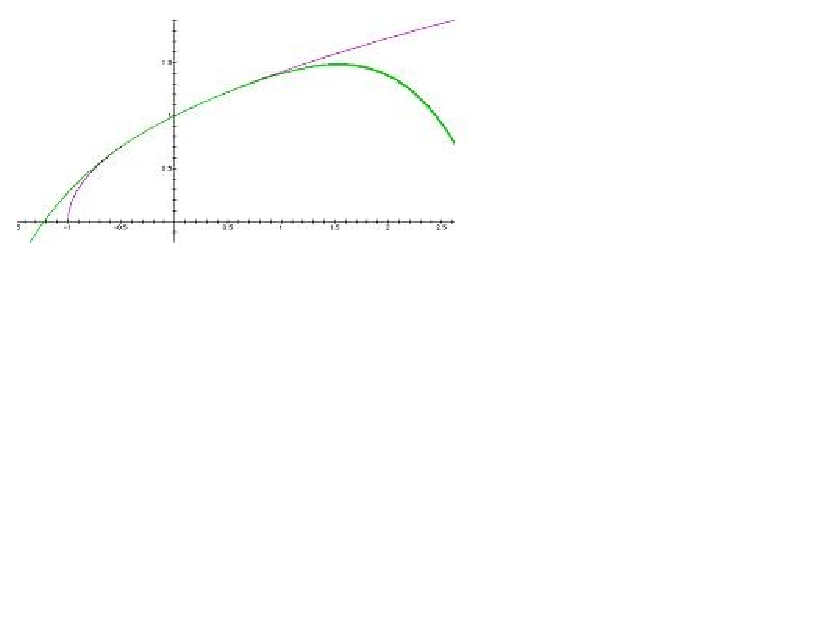
\includegraphics[width=4in]{taylorfit.eps}\\
  \caption{Taylor polynomial and $\sqrt{1+x}$}\label{f-taylor1}
\end{figure}



\textbf{Example}

Problem 1.1-8
\beqn
f(x) &=& \frac{\log(1+x)}{x} \\
&\approx & \frac{\sum_{k=1}^n\frac{(-1)^{k-1}}{k}x^k}{x} \\
&=& \sum_{k=1}^n\frac{(-1)^{k-1}}{k}x^{k-1} \\
f(0) &\approx & 1
\eeqn


\section{Remainder}
The Taylor Series obviously has errors in its approximation.  If the
original function is in $C_{n+1}$ on the interval $\alpha\leq x\leq\beta$ (with $a$ in the
interval) then the remainder (or error) is given by
\beqn
R_n(x) &=& f(x)-p_n(x) \\
&=& \frac{(x-a)^{n+1}}{(n+1)!}f^{(n+1)}(c_x)
\eeqn
with $c_x$ between $a$ and $x$.  To get an error bound we assume that $c_x$ is the worst possible.

\textbf{Example}

Problem 1.2-3(a)
In this case $n=1$ so the worst case would be if $\cos(c_x)=-1$ were $-1$.
\beqn
R_n(x)=\frac{x^{2(1)+1}}{(2(1)+1)!}=\frac{x^3}{6}\leq\frac{\pi^3}{324}<0.081
\eeqn

\textbf{Example}

Prove problem 8.


\section{Evaluating Polynomials}

Consider the polynomial
\beqn
y=a_nx^n+a_{n-1}x^{n-1}+\ldots+a_1x+a_0
\eeqn

\subsection{Straightforward}
The obvious way is to calculate each term separately,
\beqn
a_kx^k=a_k*x*x*...*x
\eeqn
This takes $k$ multiplications for a monomial of size $k$, so for a polynomial with monomials up to size $n$ it would take $\frac{n(n+1)}{2}$ multiplications.

\subsection{Storing}
Calculate $x2=x*x$, $x3=x*x2$, etc. This takes $2n-1$ multiplications.  This is much better that the straightforward way.  We can even do this without having to store each intermediate result by using a temporary variable.  Still it is not the best.

\subsection{Nesting}

Rewrite the polynomial as
\beqn
y&=&a_nx^n+a_{n-1}x^{n-1}+\ldots+a_1x+a_0 \\
&=&((\ldots(((a_n)x+a_{n-1})x+a_{n-2})\ldots)x+a_1)x+a_0.
\eeqn
This can be done as
\beqn
b_n&=&a_n \\
b_{n-1}&=&b_nx+a_{n-1} \\
b_{n-2}&=&b_{n-1}x+a_{n-2} \\
&\vdots & \\
b_1&=&b_2x+a_1 \\
b_0&=&b_1x+a_0
\eeqn
Each step takes 1 multiply so this method takes only n multiplications.  The real savings come when you have to calculate a large polynomial many times.  Another interesting thing is this is a more accurate method,  see Fig~\ref{f-polyeval}, where the dark blue line is the nested multiplication method.  Note on the right side both methods are equally good (or bad in my opinion), but on the right the nested multiplication technique shows marked improvement in accuracy.  Not bad for less work.


\begin{figure}[h]
  % Requires \usepackage{graphicx}
  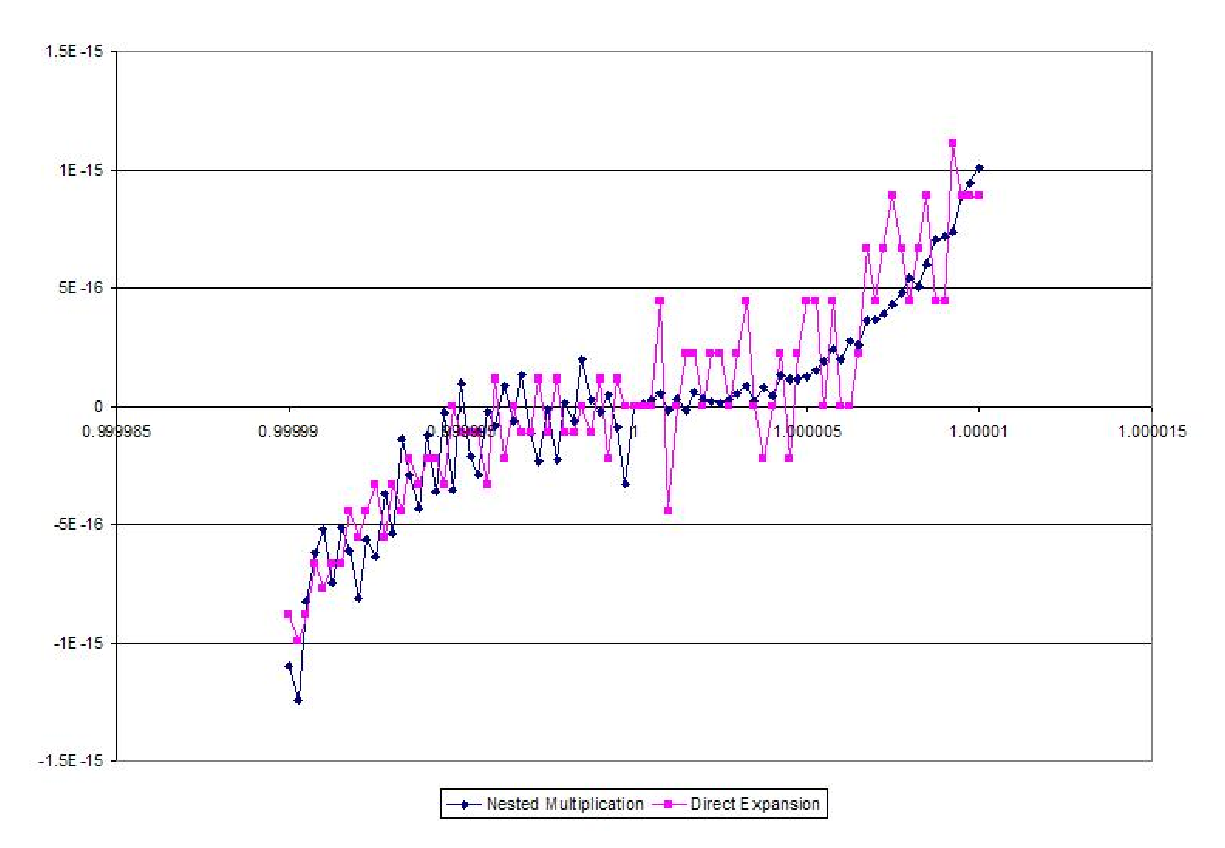
\includegraphics[width=4in]{cubicpoly.eps}\\
  \caption{Close-up Look at Resulting Values of Two Evaluation Methods for $y=x^3-3x^2+3x-1$}\label{f-polyeval}
\end{figure}



\section{Binary}
In any number system, the position of a digit relative to the decimal place specifies the integer power of the base we must multiple the digit by to get its value.  We specify what base we are using by a subscript, if no subscript appears then the base is obvious(usually base 10, though sometimes it will be base 2 if we are calculating in base 2 for that section).  So for base 10
\beqn
101_{10}=1\times 10^2 + 0\times 10^1 + 1\times 10^0,
\eeqn
and for base 2
\beqn
101_2=1\times 2^2 + 0\times 2^1 + 1\times 2^0=5_{10}.
\eeqn
This gives us one way to convert numbers.  For instance, we can convert
binary to decimal by expanding the binary number in this way.  Thus using
the above to convert binary (10.01) to decimal we find,

Note that the ``2'' we are using is the base of binary in decimal form, and this is why we went from binary to decimal.  In binary, its form would be ``10'' and ten would be ``1010''. Therefore, we could go to binary by, expanding this out with ten in binary.  The problem with this method is it is clumsy to use since we do not do squaring, cubing, etc. easily in base 2.  Another problem is that 0.1 is an infinitely repeating decimal in binary so it is a pain to deal with 10-1!  Instead, we convert decimal to binary as follows.
\begin{enumerate}
\item Split your number into a.b
\item For the whole number part, a
  \begin{enumerate}
  \item Divide 2 into a and note the quotient and remainder as q1,r1 (a=2*q1+r1)
  \item As long as the quotient from above is not zero, divide it by 2 and
record the quotient and remainder as qi,ri (with i denoting the current
step).  Repeat.
  \item The binary equivalent of a is rnrn-1...r2r1.  Basically we have done
our nested polynomial evaluation backwards with x=2, and the coefficients
being the remainders.
  \end{enumerate}
\item For the fractional part (b)
  \begin{enumerate}
  \item Multiply 2*b, and record the unit value as a1.  Denote b-a1=b1.
  \item If bi does not equal zero, multiply it by 2, denoting the units digit
by ai+1 and the difference bi-ai+1=bi+1.  Repeat until the difference is
zero (this may never happen so be looking for patterns to get repeating
fractions).
  \item The fractional part, b, is a1a2a3a4...
\end{enumerate}
\item The full answer is thus rnrn-1...r2r1.a1a2a3a4...
\end{enumerate}

\section{Hexadecimal}
This is often made to sound more intimidating than it is.  Hexadecimal
numbers are simply base 16, but this can be handled nicely since $2^4=16$.
All you have to do is group binary digits into groups of 4 and use the
conversion table

\begin{table}
  \centering
  \caption{Binary, Decimal, and Hexadecimal Equivalents}\label{t-bindechex}

\begin{tabular}{|lll|lll|} \hline
Bin  & Hex & Dec & Bin & Hex & Dec \\ \hline
0000 & 0    & 0    & 1000 & 8    & 8    \\
0001 & 1    & 1    & 1001 & 9    & 9    \\
0010 & 2    & 2    & 1010 & A    & 10   \\
0011 & 3    & 3    & 1011 & B    & 11   \\ \hline
0100 & 4    & 4    & 1100 & C    & 12   \\
0101 & 5    & 5    & 1101 & D    & 13   \\
0110 & 6    & 6    & 1110 & E    & 14   \\
0111 & 7    & 7    & 1111 & F    & 15   \\ \hline
\end{tabular}

\end{table}

\section{Fixed Point Numbers}


\vspace{.1in}\noindent
\textbf{Example:}


Convert $\pi$ to binary and hexadecimal.  Assume you have four
bits before the radix point and 8 bits after the radix point.

Sol:

before the decimal we have $3=0011$

after the decimal

\begin{tabular}{l|l}
$0.1415926\ldots$ & \\
\hline
$0.2831852$ & 0 \\
$0.5663704$ & 0 \\
$1.1327408$ & 1 \\
$0.2654816$ & 0 \\
$0.5309632$ & 0 \\
$1.0619264$ & 1 \\
$0.1238528$ & 0 \\
$0.2477056$ & 0 \\
\end{tabular}

combining gives $0011.00100100$

To convert to hexadecimal we group the digits together in groups of four starting at the radix point, thus we are forcing the hexadecimal digits to represent either integer or fractional portions.

\begin{tabular}{|c|c|c|}\hline
0011 & 0010 & 0100 \\ \hline
3    & 2    & 4    \\ \hline
\end{tabular}

Thus the answer is $0x3.24$.




\vspace{.1in}\noindent
\textbf{Example:}


Convert 25.6875 to binary.

    {\color{ans}
    \begin{tabular}{r|lcr|l}
    25 & /2 &.& *2 & .6875 \\ \hline
    12 & 1  & &  1 & .375  \\
     6 & 0  & &  0 & .75   \\
     3 & 0  & &  1 & .5    \\
     1 & 1  & &  1 & 0     \\
     0 & 1  & &    &
     \end{tabular}

     11001.1011
    }



\section{Floating point numbers}
While the book discusses single precision numbers, they are essentially never used, as double precision is so much better and readily available.  We will assume IEEE double precision floating point representation, as it is the standard.  IEEE floating point numbers have the form
\beqn
(-1)^s2^E(b_0.b_{-1}b_{-2}\ldots b_{1-p}),
\eeqn
where
\beqn
s&\in& \{0,1\} \\
s&\in& \{0,1\} \\
b_0&=&1 \,(implicitly) \\
b_{-j}&\in& \{0,1\}\forall j\in\{1,2,\ldots p-1\} \\
\eeqn

\begin{tabular}{lrr}
          & \multicolumn{2}{c}{Precision} \\
          & Single         & Double       \\
P         & 24             & 53           \\
$E_{min}$ & -126           & -1022        \\
$E_{max}$ & 127            & 1023         \\
$Bias$    & 127            & 1023         \\
\end{tabular}

Thus IEEE is represented in memory as a sign bit, exponent bits (8 or 11), and mantissa bits (23 or 52).  The mantissa is composed of all the $b_{-j}$.  A few things to note about IEEE arithmetic.
\begin{enumerate}
\item The exponent stored is $E=e-Bias$
\item $\pm 0$ is encoded by $E_{min}-1$ and $f=0$
\item Denormalized numbers are encoded by $E_{min}-1$ and $f\ne 0$
\item $\pm\infty$ is encoded by $E_{max}+1$ and $f=0$
\item NAN is encoded by $E_{max}+1$ and $f\ne 0$
\end{enumerate}

\subsection{Approximating the Reals}
To approximate the real number x, we define the function fl(x) as, 0 when x=0, and the nearest element in floating point to x otherwise.  Finding nearest elements requires a rounding scheme (rounding or ``chopping''/truncating) and a tie breaker procedure (usually round away from zero).

\subsection{Bounding Errors}
To bound the error in approximating the real number $x$, we need to consider the floating point number, $fl(x)$, used to approximate $x$.  First we note that a real number $x$, is written in binary as
\beqn
x=\sigma\cdot f_r\cdot 2^e,
\eeqn
where $\sigma$ is the sign, $f_r$ has as many digits as needed, and $e$ is any integer.  Note that $e$ will be different for IEEE, which normalizes to $1\leq f_r<2$ with an implicit 1 at the start; than the non-standard forms, which normalize to $0.5\leq f_r<1$ with no assumed leading 1.  We will assume that $e$ is within the permitted bounds for simplicity.  The floating-point representation is
\beqn
fl(x)=\sigma\cdot f\cdot 2^e.
\eeqn
We can now write the difference as
\beqn
x-fl(x)=\sigma\cdot (f_r-f)\cdot 2^e.
\eeqn
For the moment, we will consider the difference $f_r-f$.  Note that we are dealing with normalized numbers with $n$ bits of accuracy and an implicit leading 1 (IEEE arithmetic), while the book deals with numbers normalized between a half and one, with no implicit 1, so for us
\beqn
f_r &=& 1.\beta_{-1}\beta_{-2}\beta_{-3}\ldots\beta_{1-n}\beta_{n}\ldots \\
f_r &=& 1.\bar\beta_{-1}\bar\beta_{-2}\bar\beta_{-3}\ldots\bar\beta_{1-n}.
\eeqn
Note that the digit to the left of the decimal in $f$ is assumed to be 1, the only exception is when $f_r=1.1111...$ which would have $f=10.000...0$\footnote{We are forcing the exponent to be the same, otherwise it would always be true for non-zero numbers}.  Technically it would actually have f=1.000...0 and the exponent would be (e+1) but since we are keeping the exponent e we keep the simplification.  Note that this is equivalent to rounding 9.5 to 10.  Anyway, our real concern is the worst case of the difference, which is in all cases given by
\beqn
f_r-f = \pm 0.000\ldots 01.
\eeqn
Note that the 1 is in the $n^th$ place after the decimal\footnote{Explain}.  We rewrite
this using floating point notation as
.
We now stick this back into the expression for the difference between x
and fl(x) and obtain an upper bound by taking absolute value
.
Similarly to get a lower bound we take the negative of the absolute value,
and find

Now we note that the size of x is
.
For the book's form of the mantissa, we would have
.
The relative error is thus
.



\section{Floating Point Dangers}

I came up with the following program in my doctoral work at UCSB.

\begin{verbatim}
#include <iostream>
#include <iomanip>
#include <cmath>

using namespace std;

int main(){
    double pi, e, result;
    int i;

    e=exp(1);

    pi=atan(1)*4;

    result=pi;

    for(i=1;i<53;i++){
        result=sqrt(result);
    }

    for(i=1;i<53;i++){
        result=result*result;
    }

    cout << setiosflags(ios::showpoint | ios::fixed) << setprecision(16);
    cout << "Pi     = " << pi << endl;
    cout << "Result = " << result << endl;
    cout << "e      = " << e << endl;

    return 0;
}
\end{verbatim}

The results are

\begin{verbatim}
Pi     = 3.1415926535897931
Result = 2.7182818081824731
e      = 2.7182818284590451
Press any key to continue
\end{verbatim}

Notice that Result is $e$ to 7 significant digits, but it should be $\pi$.  This underscores the importance of being numerically aware when writing programs.


\section{IEEE 754}

Floating point numbers are based off scientific notation.  Consider a typical number in base 10 scientific notation,
\begin{eqnarray*}
  -1.23 \times 10^{3}.
\end{eqnarray*}
The number is composed of five pieces of information,
\begin{enumerate}
    \item sign of the number (-),
    \item significant or mantissa (1.23),
    \item base (10),
    \item sign of the exponent (+),
    \item magnitude of the exponent (3).
\end{enumerate}


There are two basic number formats called out in IEEE 754, single precision (float in c/c++), and double precision (double in c/c++).  In addition there are two extended formats, which are only used as intermediate results while calculating.
\vspace{6pt}

\begin{table}
  \centering
  \caption{IEEE Single Precision Floating Point}\label{t-ieee-fp}

\begin{tabular}{|c|c|c|c|}
  \hline
   e & f & Category & Interpretation \\
  \hline
    & $1\ldots 11$ & &  \\
   $1\ldots 11$ & $\vdots$ & NaN & See Codes \\
    & $0\ldots 01$ & &  \\ \hline
   $1\ldots 11$ & $0\ldots 00$ & $\pm\infty$ & $\pm\infty$ \\ \hline
   $1\ldots 10$ & $1\ldots 11$ & &  \\
   $\vdots$ & $\vdots$ & Numbers & $(-1)^s\times 1.f \times 2^{(e-127)}$ \\
   $0\ldots 01$ & $0\ldots 00$ & &  \\ \hline
    & $1\ldots 11$ & &  \\
   $0\ldots 00$ & $\vdots$ & Denormals & $(-1)^s\times 0.f \times 2^{(-126)}$ \\
    & $0\ldots 00$ & &  \\ \hline
   $0\ldots 00$ & $0\ldots 00$ & $\pm 0$ & $\pm 0$ \\ \hline
\end{tabular}
\end{table}


\begin{table}
  \centering
  \caption{IEEE Floating Point NaN Codes}\label{t-ieee-fp-nan}

\begin{tabular}{|c|c|c|}
  \hline
  Dec & Meaning                & Example \\ \hline
  1   & invalid square root    & $\sqrt{-1}$ \\
  2   & invalid addition       & $\infty + -\infty$ \\
  4   & invalid division       & $\frac{0}{0}$ \\
  8   & invalid multiplication & $0\times\infty$ \\
  9   & invalid modulo         & $x mod 0$ \\
   \hline
\end{tabular}
\end{table}

For this discussion, the notation $fl(x)$ will be used to mean the number $x$ as it is represented in floating point on a computer.


$$
(-1)^s\cdot 1.f\times 2^{e-127}
$$

\noindent
\begin{tabular}{c@{\extracolsep{5pt}}c@{}c@{}c@{}c@{}c@{}c@{}c@{}c@{}c@{}c@{}c@{}c@{}c@{}c@{}c@{}c@{}c@{}c@{}c@{}c@{}c@{}c@{}c@{}c@{}c@{}c@{}c@{}c@{}c@{}c@{}c}
  0 & 0 & 0 & 0 & 0 & 0 & 0 & 0 & 0 & 1 & 1 & 1 & 1 & 1 & 1 & 1 & 1 & 1 & 1 & 2 & 2 & 2 & 2 & 2 & 2 & 2 & 2 & 2 & 2 & 3 & 3 & 3 \\
  1 & 2 & 3 & 4 & 5 & 6 & 7 & 8 & 9 & 0 & 1 & 2 & 3 & 4 & 5 & 6 & 7 & 8 & 9 & 0 & 1 & 2 & 3 & 4 & 5 & 6 & 7 & 8 & 9 & 0 & 1 & 2 \\
  \hline
  \multicolumn{1}{|c}{s} & \multicolumn{8}{|c}{e} & \multicolumn{23}{|c|}{f} \\
  \hline
\end{tabular}


This is equivalent to saying


$$
(-1)^s\cdot 1.f\times 2^E
$$

\noindent
\begin{tabular}{c@{\extracolsep{5pt}}c@{}c@{}c@{}c@{}c@{}c@{}c@{}c@{}c@{}c@{}c@{}c@{}c@{}c@{}c@{}c@{}c@{}c@{}c@{}c@{}c@{}c@{}c@{}c@{}c@{}c@{}c@{}c@{}c@{}c@{}c}
  0 & 0 & 0 & 0 & 0 & 0 & 0 & 0 & 0 & 1 & 1 & 1 & 1 & 1 & 1 & 1 & 1 & 1 & 1 & 2 & 2 & 2 & 2 & 2 & 2 & 2 & 2 & 2 & 2 & 3 & 3 & 3 \\
  1 & 2 & 3 & 4 & 5 & 6 & 7 & 8 & 9 & 0 & 1 & 2 & 3 & 4 & 5 & 6 & 7 & 8 & 9 & 0 & 1 & 2 & 3 & 4 & 5 & 6 & 7 & 8 & 9 & 0 & 1 & 2 \\
  \hline
  \multicolumn{1}{|c}{s} & \multicolumn{8}{|c}{e=E+127} & \multicolumn{23}{|c|}{f} \\
  \hline
\end{tabular}

They are the same because $e-127=E$ is the same equation as $e=E+127$.  I think the latter is easier to use because you read $E$ from the number and want $e$.  The first form (standard for most texts) involves you guessing what number produced what you are seeing (rather than calculating it).  It is like trying to solve $y=mx+b$ for $y$ given $x$ but using the form $\frac{(y-b)}{m}=x$ to do it.  It works, just not well.  In any case, consider some examples.

\vspace{.1in}\noindent
\textbf{Example:}

Convert $7.892$ to single precision IEEE.

\noindent
Step 1: Convert 7.892 to binary

$7.892 = 111.1110010001011010000111$

%0.892
%1.784
%1.568
%1.136
%0.272
%0.544
%1.088
%0.176
%0.352
%0.704
%1.408
%0.816
%1.632
%1.264
%0.528
%1.056
%0.112
%0.224
%0.448
%0.896
%1.792
%1.584
%1.168

\noindent
Step 2: Normalize and note sign

$7.892 =(-1)^0 1.111110010001011010000111\times 2^2$

\noindent
Step 3: Calculate Excess 127 code for exponent

$e=2+127=129=10000001$

\noindent
Step 4:Round $1.f$ to 24 digits

$fl(1.111110010001011010000111)=1.11111001000101101000100$

\noindent
Step 5: Assemble


\begin{tabular}{|c@{ }|c@{\extracolsep{5pt}}c@{}c@{}c@{}c@{}c@{}c@{}c@{ \extracolsep{0pt}}|c@{\extracolsep{5pt}}c@{}c@{}c@{}c@{}c@{}c@{}c@{}c@{}c@{}c@{}c@{}c@{}c@{}c@{}c@{}c@{}c@{}c@{}c@{}c@{}c@{}c|}
\hline
0 & 1 & 0 & 0 & 0 & 0 & 0 & 0 & 1 & 1 & 1 & 1 & 1 & 1 & 0 & 0 & 1 & 0 & 0 & 0 & 1 & 0 & 1 & 1 & 0 & 1 & 0 & 0 & 0 & 1 & 0 & 0 \\
  \hline
\end{tabular}



\vspace{.1in}\noindent
\textbf{Example:}


Calculate $3.75\times 29.625$ in IEEE-754 single precision floating point.

    {\color{ans}
    Convert:

    $3.75=11.11=1.111\times 2^1$

    $29.625=11101.101=1.1101101\times 2^4$

    \vspace{12pt}
    Multiply Significants:

    \vspace{6pt}
    \begin{tabular}{cccccccccccc}
     &1.&1&1&0&1&1&0&1& & &  \\
$\times$&1.&1&1&1& & & & & & &  \\ \hline
     &1.&1&1&0&1&1&0&1& & &  \\
     &0.&1&1&1&0&1&1&0&1& &  \\
     &0.&0&1&1&1&0&1&1&0&1&  \\
     &0.&0&0&1&1&1&0&1&1&0&1 \\ \hline
    1&1.&0&1&1&1&1&0&0&0&1&1
    \end{tabular}

    $1.10111100011\times 2^1$

    \vspace{12pt}
    Add exponents to normalization exponent and put in excess 127:

    \vspace{6pt}
    $1+4+1+127=133=10000101$

    \vspace{12pt}
    Write in single precision:

    \vspace{6pt}
    \begin{tabular}{|c|c|c|}\hline 0 & 10000101 & 1011 1100 0110 0000 0000 000 \\ \hline \end{tabular}


    }






\vspace{.1in}\noindent
\textbf{Example:}

Perform the following for IEEE-754, single precision
    \begin{enumerate}
        \item Show the representation of $x=93.3125$

        {\color{ans}

        $x=93.125_{10}=1011101.001_2=1.011101001\times 2^6$

\noindent
\begin{tabular}{|c@{\extracolsep{0pt} }|c@{\extracolsep{5pt}}c@{}c@{}c@{}c@{}c@{}c@{}c@{\extracolsep{0pt} }|c@{\extracolsep{5pt}}c@{}c@{}c@{}c@{}c@{}c@{}c@{}c@{}c@{}c@{}c@{}c@{}c@{}c@{}c@{}c@{}c@{}c@{}c@{}c@{}c@{}c|}
\hline                            %
0 & 1 & 0 & 0 & 0 & 0 & 1 & 0 & 1 & 0 & 1 & 1 & 1 & 0 & 1 & 0 & 0 & 1 & 0 & 0 & 0 & 0 & 0 & 0 & 0 & 0 & 0 & 0 & 0 & 0 & 0 & 0 \\
  \hline
\end{tabular}
        }

        \item calculate $x*y$ for $y$ equal to

\noindent
\begin{tabular}{|c@{\extracolsep{0pt} }|c@{\extracolsep{5pt}}c@{}c@{}c@{}c@{}c@{}c@{}c@{\extracolsep{0pt} }|c@{\extracolsep{5pt}}c@{}c@{}c@{}c@{}c@{}c@{}c@{}c@{}c@{}c@{}c@{}c@{}c@{}c@{}c@{}c@{}c@{}c@{}c@{}c@{}c@{}c|}
\hline                            %
0 & 1 & 0 & 0 & 0 & 0 & 0 & 0 & 0 & 0 & 0 & 0 & 0 & 0 & 0 & 0 & 0 & 0 & 0 & 0 & 0 & 0 & 0 & 0 & 0 & 0 & 0 & 0 & 0 & 1 & 0 & 0 \\
  \hline
\end{tabular}

    {\color{ans}
    exponent: 128+133-127=134

    float: shortcut, note that $y$ only has two 1's in the expansion (hidden and near end) and they are farther apart than the length of the significant portion of $x$.  This will cause the $x$ float to be placed starting at these locations.  The comma below notes where the last bit of precision lies.
\begin{eqnarray*}
z_{fl} & = & 1.01110100100000000000101,1101001
\end{eqnarray*}
Note that the first bit after the comma is a 1 so the number gets rounded up.

        z is

\noindent
\begin{tabular}{|c@{\extracolsep{0pt} }|c@{\extracolsep{5pt}}c@{}c@{}c@{}c@{}c@{}c@{}c@{\extracolsep{0pt} }|c@{\extracolsep{5pt}}c@{}c@{}c@{}c@{}c@{}c@{}c@{}c@{}c@{}c@{}c@{}c@{}c@{}c@{}c@{}c@{}c@{}c@{}c@{}c@{}c@{}c|}
\hline                            %
0 & 1 & 0 & 0 & 0 & 0 & 1 & 1 & 0 & 0 & 1 & 1 & 1 & 0 & 1 & 0 & 0 & 1 & 0 & 0 & 0 & 0 & 0 & 0 & 0 & 0 & 0 & 0 & 0 & 1 & 1 & 0 \\
  \hline
\end{tabular}
    }

    \end{enumerate}



\vspace{.1in}\noindent
\textbf{Example:}

Convert 3.03125 to IEEE single precision

    {\color{ans}
    \begin{tabular}{c|ccc|c}
      3 &   & . &   & 03125 \\ \hline
      1 & 1 &   & 0 & 0625  \\
      0 & 1 &   & 0 & 125  \\
        &   &   & 0 & 25  \\
        &   &   & 0 & 5  \\
        &   &   & 1 & 0  \\
    \end{tabular}

    $3.03125_{10}=11.00001_2=1.100001_2\times 2^1$

    $1+127 = 128$

    \begin{tabular}{|c@{ }|c@{\extracolsep{5pt}}c@{}c@{}c@{}c@{}c@{}c@{}c@{ \extracolsep{0pt}}|c@{\extracolsep{5pt}}c@{}c@{}c@{}c@{}c@{}c@{}c@{}c@{}c@{}c@{}c@{}c@{}c@{}c@{}c@{}c@{}c@{}c@{}c@{}c@{}c@{}c|}
\hline
0 & 1 & 0 & 0 & 0 & 0 & 0 & 0 & 0 & 1 & 0 & 0 & 0 & 0 & 1 & 0 & 0 & 0 & 0 & 0 & 0 & 0 & 0 & 0 & 0 & 0 & 0 & 0 & 0 & 0 & 0 & 0 \\
  \hline
\end{tabular}
    }

Now perform the following on your result and

\begin{tabular}{|c@{ }|c@{\extracolsep{5pt}}c@{}c@{}c@{}c@{}c@{}c@{}c@{ \extracolsep{0pt}}|c@{\extracolsep{5pt}}c@{}c@{}c@{}c@{}c@{}c@{}c@{}c@{}c@{}c@{}c@{}c@{}c@{}c@{}c@{}c@{}c@{}c@{}c@{}c@{}c@{}c|}
\hline
0 & 1 & 0 & 0 & 0 & 0 & 1 & 0 & 0 & 0 & 0 & 0 & 0 & 0 & 0 & 0 & 1 & 0 & 0 & 0 & 0 & 0 & 0 & 0 & 1 & 0 & 0 & 0 & 0 & 0 & 0 & 0 \\
  \hline
\end{tabular}
\begin{enumerate}
    \item Addition

    {\color{ans}
    $x=1.0000000100000001_2\times 2^5$

    $y=1.100001_2\times 2^1=0.0001100001_2\times 2^5$

    \begin{eqnarray*}
    x+y & = & 1.0000000100000001_2\times 2^5+0.0001100001_2\times 2^5 \\
        & = & (1.0000000100000001_2+0.0001100001_2)\times 2^5 \\
        & = & (1.0001100101000001_2)\times 2^5
    \end{eqnarray*}

\begin{tabular}{|c@{ }|c@{\extracolsep{5pt}}c@{}c@{}c@{}c@{}c@{}c@{}c@{ \extracolsep{0pt}}|c@{\extracolsep{5pt}}c@{}c@{}c@{}c@{}c@{}c@{}c@{}c@{}c@{}c@{}c@{}c@{}c@{}c@{}c@{}c@{}c@{}c@{}c@{}c@{}c@{}c|}
\hline
0 & 1 & 0 & 0 & 0 & 0 & 1 & 0 & 0 & 0 & 0 & 0 & 1 & 1 & 0 & 0 & 1 & 0 & 1 & 0 & 0 & 0 & 0 & 0 & 1 & 0 & 0 & 0 & 0 & 0 & 0 & 0 \\
  \hline
\end{tabular}
    }

    \item Multiplication
    {\color{ans}

    exponent is $132+128-127=133$

    significant is $1.0000000100000001\times 1.100001 = 1.1000010110000101100001$

\begin{tabular}{|c@{ }|c@{\extracolsep{5pt}}c@{}c@{}c@{}c@{}c@{}c@{}c@{ \extracolsep{0pt}}|c@{\extracolsep{5pt}}c@{}c@{}c@{}c@{}c@{}c@{}c@{}c@{}c@{}c@{}c@{}c@{}c@{}c@{}c@{}c@{}c@{}c@{}c@{}c@{}c@{}c|}
\hline
0 & 1 & 0 & 0 & 0 & 0 & 1 & 0 & 1 & 1 & 0 & 0 & 0 & 0 & 1 & 0 & 1 & 1 & 0 & 0 & 0 & 0 & 1 & 0 & 1 & 1 & 0 & 0 & 0 & 0 & 1 & 0 \\
  \hline
\end{tabular}
    }

\end{enumerate}






\vspace{.1in}\noindent
\textbf{Example:}

Perform the following for IEEE-754, single precision
    \begin{enumerate}
        \item Show the representation of $x=0.8125$

        {\color{ans}

\noindent
\begin{tabular}{|c@{\extracolsep{0pt} }|c@{\extracolsep{5pt}}c@{}c@{}c@{}c@{}c@{}c@{}c@{\extracolsep{0pt} }|c@{\extracolsep{5pt}}c@{}c@{}c@{}c@{}c@{}c@{}c@{}c@{}c@{}c@{}c@{}c@{}c@{}c@{}c@{}c@{}c@{}c@{}c@{}c@{}c@{}c|}
\hline                            %
0 & 0 & 1 & 1 & 1 & 1 & 1 & 1 & 0 & 1 & 0 & 1 & 0 & 0 & 0 & 0 & 0 & 0 & 0 & 0 & 0 & 0 & 0 & 0 & 0 & 0 & 0 & 0 & 0 & 0 & 0 & 0 \\
  \hline
\end{tabular}
        }

        \item calculate (show steps) $x*y$ for $x$ from above and

        y is

\noindent
\begin{tabular}{|c@{\extracolsep{0pt} }|c@{\extracolsep{5pt}}c@{}c@{}c@{}c@{}c@{}c@{}c@{\extracolsep{0pt} }|c@{\extracolsep{5pt}}c@{}c@{}c@{}c@{}c@{}c@{}c@{}c@{}c@{}c@{}c@{}c@{}c@{}c@{}c@{}c@{}c@{}c@{}c@{}c@{}c@{}c|}
\hline                            %
1 & 1 & 0 & 0 & 0 & 0 & 0 & 0 & 1 & 1 & 1 & 0 & 0 & 0 & 0 & 0 & 0 & 0 & 0 & 0 & 0 & 0 & 0 & 0 & 0 & 0 & 0 & 0 & 0 & 0 & 0 & 0 \\
  \hline
\end{tabular}

        {\color{ans}
        Exponent: $(10000001+01111110)-01111111=11111111-01111111=1000000$

        float= $1.101*1.11=10.11011=1.011011 \times 2^1$, so add 1 to exponent

\noindent
\begin{tabular}{|c@{\extracolsep{0pt} }|c@{\extracolsep{5pt}}c@{}c@{}c@{}c@{}c@{}c@{}c@{\extracolsep{0pt} }|c@{\extracolsep{5pt}}c@{}c@{}c@{}c@{}c@{}c@{}c@{}c@{}c@{}c@{}c@{}c@{}c@{}c@{}c@{}c@{}c@{}c@{}c@{}c@{}c@{}c|}
\hline                            %
1 & 1 & 0 & 0 & 0 & 0 & 0 & 0 & 1 & 0 & 1 & 1 & 0 & 1 & 1 & 0 & 0 & 0 & 0 & 0 & 0 & 0 & 0 & 0 & 0 & 0 & 0 & 0 & 0 & 0 & 0 & 0 \\
  \hline
\end{tabular}
        }

        \item Perform the multiplication above in decimal and verify the answer.

        {\color{ans}
        $.8125*(-7)=-5.6875=-101.1011_2$
        }

    \end{enumerate}

\section{Rounding versus Chopping}

Rounding is almost always used because of two reasons.  To see both, let the interval between two numbers in the representation is $2\delta$ then for rounding $x-fl(x)\in [-\delta,\delta)$, while for chopping it is $x-fl(x)\in [0,2\delta)$.  The first problem is that the error magnitude is up to twice as large for chopping.  This is obviously bad, but it is not as bad as the second problem.  The second problem is that all the errors of chopping have the same sign, so no error cancellation is possible when calculations are done.  To see why this is bad, consider the following.

\vspace{.1in}\noindent
\textbf{Example:}

Find out the error in calculating $\sum_{i=1}^{n}x_i$ on a computer.  First note that what you actually calculate is $\sum_{i=1}^{n}fl(x_i)$.  The error (actual minus calculated) is thus $Err=\left|(\sum_{i=1}^{n}x_i)-(\sum_{i=1}^{n}fl(x_i))\right|$.  Also let $fl(x_i)=x_i+\gamma_i$ for $\gamma_i$ in the error interval of your method.

\begin{eqnarray*}
  Err &=& \left|(\sum_{i=1}^{n}x_i)-(\sum_{i=1}^{n}(x_i+\gamma_i))\right| \\
    &=& \left|(\sum_{i=1}^{n}x_i)-(\sum_{i=1}^{n}x_i+\sum_{i=1}^{n}\gamma_i)\right| \\
    &=& \left|\sum_{i=1}^{n}x_i-\sum_{i=1}^{n}x_i-\sum_{i=1}^{n}\gamma_i\right| \\
    &=& \left|\sum_{i=1}^{n}\gamma_i\right| \\
    &\leq & \sum_{i=1}^{n}\left|\gamma_i\right|
\end{eqnarray*}

For chopping the last inequality is actually an equality, i.e. chopping always has the worst case error.  For a typical case on rounding the errors are distributed with some positive and some negative, thus cancelation can occur.  For large sums (many terms) the law of large numbers and an assumed uniform distribution of $\gamma_i$ indicates that the error for rounding will go to $0$!  This is a great result.

\section{Absolute and Relative Error}

The two most basic types of errors are absolute and relative.  The absolute error of an estimate $\hat x$ of a number $x$, is the difference between them.
\begin{eqnarray}
AE&=&\Delta x\\
  &=&x-\hat x
\end{eqnarray}
The relative error of an estimate $\hat x$ of a number $x$, is the difference between them divided by $x$.
\begin{eqnarray}
RE&=&\frac{\Delta x}{x}\\
  &=&\frac{x-\hat x}{x}
\end{eqnarray}
Often the the absolute value of either the absolute or relative error is taken, though not in every case, so it is important to know if only the magnitude or magnitude and phase (sign) is required.  Unfortunately, there is no standard nomenclature or convention, though more often than not the magnitude (take the absolute value) is desired. Usually the phase/sign information is only retained in the error if it is plausible to have and will be useful in the algorithm or analysis.

\section{Propagation of Error}
We have seen that representing the real numbers on a computer involves errors.  When we use floating point numbers in a calculation rather than the actual numbers the errors can grow.  The errors caused by using floating point approximations are called propagated errors.  Two ways of bounding propagation errors exist.  The forward method involves explicitly calculating the errors and is called interval arithmetic.  The backward method involves finding a condition number, which gives a bound on how big the error can grow.

\section{Interval Arithmetic}

Let's consider the error in a computation between the true values (xT, yT) and the approximate values (xA, yA).  We only know the approximate values and the error bounds

Note that the error is could be positive or negative so we must consider the positive and negative bounds.  First, we will look at the error for addition or subtraction.

Now let's consider multiplication.

It is easy to see that this can quickly become very hard to deal with.  Consider for instance multiplying two n-by-n matrices, which would involve $n^{3}$ multiplies.  Keeping track of all of them would rapidly become impossible.  We will consider one final operation, namely division.

Again we can see that things can become very complicated quickly.

\section{Forward and Backward Error}

Two other distinctions in error types that come up in stability of algorithms are forward and backward errors.  They are concerned with a piece of data, $x$, that is acted on by an equation or algorithm, $f(\cdot)$ to produce a result, $y$.
\begin{eqnarray}
y&=&f(x)
\end{eqnarray}
This probably seems pretty straight-forward, but what happens when I can't actually calculate $f(\cdot)$?  For instance, how can I calculate a transcendental function\footnote{Transcendental functions cannot be expressed as a finite sequence of algebraic operations - arithmetic and roots} like $\sin(x)$?  The answer is we have to approximate the equation or algorithm with another one that is calculable on a computer.  We will examine some ways to do this later, but first we need a way to see how good our approximation is, which is what forward and backward errors gives us.  We will denote our approximate algorithm by $\hat f(\cdot)$.  Now if we give our approximate algorithm the true starting value of $x$, what it calculates will not be $y$ but $\hat y$.
\begin{eqnarray}
\hat y&=&\hat f(x)
\end{eqnarray}
The error of the results, given the same starting point, gives us an idea of how good our approximation is.  If it is small then we say the algorithm is stable.  The difference of the values calculated is the forward error.
\begin{eqnarray*}
FE_{abs}&=&\Delta y\\
        &=& y-\hat y\\
        &=& f(x)-\hat(x)\\
FE_{rel}&=&\frac{\Delta y}{y}\\
        &=& \frac{y-\hat y}{y}\\
        &=& \frac{f(x)-\hat f(x)}{f(x)}
\end{eqnarray*}
In general we will use the relative forward error, though you could use either.  Forward error is a useful and intuitive concept, but it is not always easy to quantify for a range of values, since you have to explicitly calculate for each one.  This makes it less useful for algorithm analysis.  Enter the backward error.  Its definition will seem weird and probably even more difficult, but it turns out to be easy in many cases to bound for a wide range of problems.  In other words we use it because it makes our lives easy.

The backward error is the smallest value, $\Delta x$ such that
\begin{eqnarray}
f(\hat x) &=& \hat f(x)\\
\hat x &=& x+\Delta x
\end{eqnarray}
holds.  Solving this we find
\begin{eqnarray*}
f(x+\Delta x) &=& \hat f(x)\\
x+\Delta x &=& f^{-1}\left(\hat f(x)\right)\\
\Delta x &=& f^{-1}\left(\hat f(x)\right)-x.
\end{eqnarray*}
The absolute backward error is $\Delta x$ and the relative backward error is $\frac{\Delta x}{x}$.

\section{Condition Number}
To make this a little more understandable, I am going to draw a distinction not used in the literature\footnote{This warning exists only to prevent you from expecting others to know or use this, though it is much clearer in my mind.}, that of condition number at a point and condition number of an algorithm.  The condition number of an algorithm is the worst condition number at a point for all the possible points, thus
\begin{eqnarray}
cond(f) &=& \sup_x cond(f(x))
\end{eqnarray}
The condition number at a point is then how much the output changes given a change in the input, thus it is a ratio of the relative forward error over the relative backward error.
\begin{eqnarray*}
cond(f(x)) &=& \left|\frac{\frac{y-\hat y}{y}}{\frac{x-\hat x}{x}}\right| \\
           &=& \left|\frac{\frac{f(x)-\hat f(x)}{f(x)}}{\frac{x-f^{-1}(\hat f(x))}{x}}\right|
\end{eqnarray*}
Note that by definition of the backward error, we have $f(\hat x) = \hat f(x)$ and $\Delta x= x-\hat x$.
\begin{eqnarray*}
cond(f(x)) &=& \left|\frac{\frac{f(x)-f(\hat x)}{f(x)}}{\frac{\Delta x}{x}}\right|
\end{eqnarray*}
In this form it looks a lot like a calculus formula, which suggests using the derivative to simplify the equation.  This of course requires the derivative to exist.  Recall that 
\begin{eqnarray*}
f'(x)&=&lim_{\Delta x\rightarrow 0}\frac{f(x)-f(x+\Delta x)}{\Delta x}.
\end{eqnarray*}
We don't have a limit, so we can only approximate this
\begin{eqnarray*}
f'(x)&\approx&\frac{f(x)-f(x+\Delta x)}{\Delta x}
\end{eqnarray*}
thus
\begin{eqnarray*}
cond(f(x)) &=& \left|\frac{\frac{f(x)-f(\hat x)}{f(x)}}{\frac{\Delta x}{x}}\right| \\
           &=& \left|\frac{f(x)-f(\hat x)}{\Delta x}\frac{x}{f(x)}\right| \\
           &=& \left|\frac{f(x)-f(x+\Delta x)}{\Delta x}\frac{x}{f(x)}\right| \\
           &\approx& \left|f'(x)\frac{x}{f(x)}\right|
\end{eqnarray*}
The condition number at a point thus gives us how the errors grow at that point, and the condition number of the function gives us the worst case bound on how bad our errors can grow.

Note this is not the only way we could have developed this.  We could have required our
function to be continuous on [$x$,$\hat x$] and differentiable on ($x$,$\hat x$), which is looser than the completely differentiable requirement I made above.  We can thus use the mean value theorem to see
\begin{eqnarray*}
f'(c)&=&\frac{f(x)-f(\hat x)}{x-\hat x}
\end{eqnarray*}
We now note that since $c$ is between the true, $x$, and approximate, $\hat x$ values, and that the interval is on the order of $10^{-16}$ for IEEE double-precision arithmetic.  We can thus assume $c$ is approximately $x$.
\begin{eqnarray*}
f'(x)&\approx&\frac{f(x)-f(\hat x)}{x-\hat x}
\end{eqnarray*}
The derivative of $f(x)$ at $x$, is called the absolute condition number.  To get the relative condition number you just have to divide each of the differences by their true value, which works out to multiplying by $\frac{x}{f(x)}$, thus
\begin{eqnarray*}
cond(f(x)) &\approx& \left|f'(x)\frac{x}{f(x)}\right|
\end{eqnarray*}
Same equation either way.

The condition number shows how the error of the approximation will influence the error of the calculation.    The condition number is nice in that it cleanly handles the error bounds.  It is not as precise as the error in the interval arithmetic, but it is tractable even for large matrix operations, which will involve the norms of the matrices rather than the elements.  Quite a
savings!

\subsection{Sums}
We have spoken a lot about summation, but we want to look at one final
area of sums before we move on.  Consider the following summation:
\begin{eqnarray}
100000+45+45+45+45
\end{eqnarray}
In real numbers it doesn't matter if we add the 45's first or the 100000.
In floating point numbers it does matter!  Floating point numbers are not
associative.  To see this consider a 4 decimal place accuracy machine that
uses rounding, and is nicely implemented.  In this case we see that
\beqn
100000+45=100000
\eeqn
so if we add as stated we find the sum is 100000 for the series (rather
than 100180).  If we add the 45's first we find that
\beqn
45+45+45+45=180,
\eeqn
then
\beqn
100000+180=100200.
\eeqn
A much better result.  These sums occur in a variety of places, from
standard series, to evaluating integrals, to inner products of vector, and
matrix multiplication.  In short you should be aware of the lack of the
associative property.


\vspace{.1in}\noindent
\textbf{Example}

Write C/C++ code to sum the following $\sum_{i=1}^{100}\frac{1}{i^2}$.  Make sure you do it in the right order.
    {\color{ans}

    \begin{verbatim}
    double sum=0;
    int i;

    for(i=100;i>=0;i--){
        sum+=1.0/(i*i);}
    \end{verbatim}

    }

\subsubsection{Kahan's Compensated Summation}

\SciLab{Kahan's Compensated Summation}{sci:kahan-comp-sum}{scilab/compsum.sci} 
Almost every interesting problem in mathematics can be reduced to trying 
to find the zeros of a function.  The next several classes will be spent 
examining how we find zeros.  In general, you cannot explicitly solve for 
the zeros so you need to make iterative procedures to find them.  Today we 
will look at two methods: bisection and Newton's method.
\section{Bisection}
Bisection is a nice method in that it is guaranteed to converge and you 
can state exactly how many iterations it will take.


\section{Newton's Method}
Newton's Method essentially is an algebraic re-writing of the tangent line 
of a function at a point.

We can then use Taylor's formula to obtain an error bound.
\section{Secant}
Newton's Method requires the knowledge of the first derivative of the 
function.  Often the derivative is very complicated to evaluate and 
will take a long (relatively anyway) time to do so.  In many cases the 
first derivative may not be available.  In some cases it might not even 
exist at all points in the interval of interest.  Even when it is 
available it could be near zero which would cause numerical problems 
in evaluating it, even if it is in the region of convergence.  For 
all of these regions a new method was devised, which drew on the 
material leading up to calculus.  

Recall that the tangent line was 
found as the limit of a series of secant lines.  We can say that the 
derivative can thus be approximated by
\beqn
f(x)\approx\frac{f(x_{1})-f(x_{2})}{x_{1}-x_{2}}.
\eeqn
Thus if we know two points, we can approximate the funciton by a 
straight line between them and use the x-intercept as the next point 
to evaluate.  We now need two points instead of one and a 
derivative.  We refer to this as a two-point method because of the 
need of multiple points.  We will need two estimates to begin our 
evaluation.  Given two initial gueses, $x_{0}$ and $x_{1}$, the slope, 
$m$, is given by
\beqn
m=\frac{f(x_{1})-f(x_{0})}{x_{1}-x_{0}}.
\eeqn
Using this we find the next point, $x_{2}$ by using the point-slope 
form of a line
\beqn
f(x_{2})-f(x_{1}) & = & 
  \frac{f(x_{1})-f(x_{0})}{x_{1}-x_{0}}(x_{2}- x_{1}) \\
x_{2}- x_{1} & = & 
  \frac{x_{1}-x_{0}}{f(x_{1})-f(x_{0})}(f(x_{2})-f(x_{1})) \\
x_{2} & = & 
  x_{1}-f(x_{1})\frac{x_{1}-x_{0}}{f(x_{1})-f(x_{0})}. 
\eeqn
We thus have the equation for the next estimate:
\beq
x_{n+1} = 
  x_{n}-f(x_{n})\frac{x_{n}-x_{n-1}}{f(x_{n})-f(x_{n-1})}. \label{eq-sec1}
\eeq
Note that you can store the previous function evaluation and then you 
will not need to do two function evaluations per iteration.

Now we want to calculate the error.  To do this we will subtract 
eq~\ref{eq-sec1} from $\alpha=\alpha$.
\beqn
e_{n+1} & = & \alpha - x_{n+1} \\
  & = & \alpha -
    \left(x_{n}-f(x_{n})\frac{x_{n}-x_{n-1}}{f(x_{n})-f(x_{n-1})}\right) \\
  & = & \alpha -\frac{f(x_{n})x_{n-1}-f(x_{n-1})x_{n}}{f(x_{n})-f(x_{n-1})} \\
  & = & \frac{f(x_{n})(\alpha -x_{n-1})-f(x_{n-1})(\alpha -x_{n})}
       {f(x_{n})-f(x_{n-1})} \\
  & = & \frac{f(x_{n})e_{n-1}-f(x_{n-1})e_{n}}{f(x_{n})-f(x_{n-1})} \\
  & = & e_{n} e_{n-1}\frac{\frac{f(x_{n})}{e_{n}}-\frac{f(x_{n-1})}{e_{n-1}}}
       {f(x_{n})-f(x_{n-1})} \\
  & = & e_{n} e_{n-1}\frac{\frac{f(x_{n})}{e_{n}}-\frac{f(x_{n-1})}{e_{n-1}}}
       {x_{n}-x_{n-1}}\frac{x_{n}-x_{n-1}}{f(x_{n})-f(x_{n-1})} \\
  & \approx & e_{n} e_{n-1}\frac{\frac{f(x_{n})}{e_{n}}-\frac{f(x_{n-1})}{e_{n-1}}}
       {x_{n}-x_{n-1}}\frac{1}{f'(\alpha)}
\eeqn
We need to evaluate $\frac{f(x_{n})}{e_{n}}$, so we will use Taylor's 
Theorem for $f(x)$ evaluated at $\alpha$.  We find that
\beqn
\frac{f(x_{n})}{e_{n}} & = & 
\frac{f(\alpha)+(\alpha-x_{n})f'(\alpha)+\frac{1}{2}
  (\alpha-x_{n})^{2}f''(\alpha)+{\cal O}((\alpha-x_{n})^{3})}{e_{n}} \\
& = & 
\frac{e_{n}f'(\alpha)+\frac{1}{2}e_{n}^{2}f''(\alpha)
   +{\cal O}(e_{n}^{3})}{e_{n}} \\
& = & 
f'(\alpha)+\frac{1}{2}e_{n}f''(\alpha)+{\cal O}(e_{n}^{2})
\eeqn
Resuming our evaluation of $e_{n+1}$ we find
\beqn
e_{n+1} 
  & \approx & e_{n} e_{n-1}\frac
  {f'(\alpha)+\frac{1}{2}e_{n}f''(\alpha)+{\cal O}(e_{n}^{2})
  -f'(\alpha)-\frac{1}{2}e_{n-1}f''(\alpha)+{\cal O}(e_{n-1}^{2})}
       {x_{n}-x_{n-1}}\frac{1}{f'(\alpha)} \\
  & = & e_{n} e_{n-1}\frac{\frac{1}{2}e_{n}f''(\alpha)
   -\frac{1}{2}e_{n-1}f''(\alpha)+{\cal O}(e_{n-1}^{2})}
       {x_{n}-x_{n-1}}\frac{1}{f'(\alpha)} \\
  & = & e_{n} e_{n-1}\frac{\frac{1}{2}(e_{n}-e_{n-1})f''(\alpha)
   +{\cal O}(e_{n-1}^{2})}{x_{n}-x_{n-1}}\frac{1}{f'(\alpha)} \\
  & = & e_{n} e_{n-1}\frac{\frac{1}{2}(x_{n}-x_{n-1})f''(\alpha)
   +{\cal O}(e_{n-1}^{2})}{x_{n}-x_{n-1}}\frac{1}{f'(\alpha)} \\
  & = & e_{n} e_{n-1}(\frac{1}{2}f''(\alpha)
   +{\cal O}(e_{n-1}^{2}))\frac{1}{f'(\alpha)} \\
  & \approx & e_{n}e_{n-1}\frac{f''(\alpha)}{2f'(\alpha)} \\
  & \approx & e_{n}e_{n-1}M.
\eeqn
This is similar to Newton's method which suggests that
\beqn
  e_{n+1}=Ae_{n}^{c},
\eeqn
which implies
\beqn
  e_{n}=A^{-1}e_{n-1}^{c^{-1}}.
\eeqn
Substituting and collecting terms we find
\beqn
B=e_{n}^{1-c+c^{-1}}.
\eeqn
Since the left hand side is a constant the exponent must be zero, or 
$c$ must be the golden ratio.
This implies that the secant method converges superlinearly.
\section{Regula Falsi}


\section{Fixed Points}
A fixed point is a point in the domain of a function, which maps its 
domain back into its domain, that satisfies $\alpha=C(\alpha)$.  
Since $\alpha$ does not change when it is mapped by the function it is 
fixed, hence the name.  We need to look at what 
the idea that underlies fixed points: contractions.  A contraction 
$y=C(x)$, is a mapping from a closed interval in $X$ into another closed 
interval in $Y$ with the property that for some $b=C(a)$ (usually $a$ 
and $b$ are both the origin but it is not required), $\|\cdot\|_{x}$ 
a norm on $X$, and $\|\cdot\|_{y}$ a norm on $Y$ we have:
\beqn
\| x-a\|_{x} > \| y-b\|_{y} = \| C(x)-C(a)\|_{y}
\eeqn
for all $x\in X$ and $y\in Y$.  Usually we have $X$ and $Y$ are $\Re$ 
and $a=b$, which gives us that $|x-a|>|C(x)-a|$.  Take the derivative of both 
sides and we see 
\beqn
1>|C'(x)|.
\eeqn
This brings up a key point, we must have that the magnitude of the 
function's slope is less than 1.  If you think about this it makes 
sense, as for slope magnitudes greater than one there will be growth 
and we are looking a funcions which shrink things.  While this is a 
simple idea, it has many profound implications.  The book proves 
nicely how the uniqueness of solution, convergence, etc..  One thing 
that should be highlated has to do with rate of convergence.  Given a 
contraction defined on an interval $[a,b]$ with some point, $\alpha = 
C(\alpha)\in[a,b]$ called a fixed point, we can define the iteration 
$x_{n+1}=C(x_{n})$.  We then have (using the mean value theorem)
\beqn
\alpha-x_{n+1} 
 & = & C(\alpha)-C(x_{n}) \\
 & = & C'(d)(\alpha-x_{n}) \\
|\alpha-x_{n+1}| 
 & < & |\alpha-x_{n}|.
\eeqn
We have linear convergence from this.  Consider the following paradox.

Let a function $g(x)$ be defined by
\beqn
g(x)=x-\frac{f(x)}{f'(x)}
\eeqn
and let $f(x)$ have a single root in some interval $[a,b]$.  From the 
book we know this must have a fixed point in the interval and the 
iteration $x_{n+1}=g(x_{n})$ will converge to the fixed point.  This 
method thus has linear convergence from what we have proven above.  
This iteration is Newton's Method though, so it has Quadratic 
convergence.  What gives?  The convergence of a fixed point algorithm 
is at least linear but it can be better if $C'(\alpha)=0$.  Notice 
that the derivative of $g(x)$ is given by
\beqn
g'(x) & = & 1-\frac{(f'(x))^{2}-f(x)f''(x)}{(f'(x))^{2}} \\
      & = & \frac{f(x)f''(x)}{(f'(x))^{2}}.
\eeqn
Note that for $x=\alpha$ we trivially have that $g'(\alpha)=0$, which 
satisfies our requirement for faster convergence.

How can I get a function $g(x)$ that satisfies the requirements?  
Many ways exist but consider the following.  For a function $f(x)$ with 
a zero at $x=\alpha$ in an interval $[a,b]$, that has 
$\beta=\max_{x\in[a,b]}|f'(x)|$, we define the iteration
\beqn
x_{n+1}=x_{n}-\gamma sign(f'(x_{n}))f(x_{n})
\eeqn
with $0<\gamma\beta<2$.  We then see that
\beqn
g(x) & = & x-\gamma sign(f'(x))f(x) \\
g'(x) & = & 1-\gamma sign(f'(x))f'(x) \\
      & = & 1-\gamma |f'(x)|
\eeqn
and thus $1>g'(x)>-1$.  Note that if we choose $\gamma$ such that 
$0<\gamma\beta<1$ then $1>g'(x)>0$ and the sequence 
$\{x_{i}\}_{i=0}^{\infty}$ converges to $\alpha$ from one side (no 
alternating).  The parameter $\gamma$ is refered to as the {\bf step 
size}.  As a final note, we can use Aitken's $\Delta^{2}$ method as 
outlined in the book to refine the estimate $x_{n}$.  Replace $\alpha$ 
with $\hat{x}_{n}$ and you have a refinement and acceleration method 
that will work on any linearly convergent algorithm.  It can thus be 
used on general fixed point methods.

Homework 
4.3: 6, 13
\newpage
\section{Continuation Methods}
One of the essential problems in root finding is to find a good place 
to start.  We have spoken about the progressively doubling intervals 
till we find a sign change.  I mentioned this was not the fastest or 
best, but would work.  I wanted to give you what I think is one of the 
best.  It is refered to as a continuation method or sometimes a 
homotopy.

A homotopy, $h$, is a continuous connection between two functions, $f$ and 
$g$, that maps one space, $X$, to another, $Y$:
\beqn
h:[0,1]\times X\rightarrow Y
\eeqn
such that $h(0,x)=g(x)$ and $h(1,x)=f(x)$.  Two simple homotopies we will 
use are listed below.
\begin{enumerate}
\item
\beqn
h(\lambda,x)=\lambda f(x)+(1-\lambda)g(x)
\eeqn
\item
\beqn
h(\lambda,x) & = & \lambda f(x)+(1-\lambda)(f(x)-f(\alpha_{0})) \\
             & = & f(x)-(1-\lambda)f(\alpha_{0})
\eeqn
\end{enumerate}
The first one is the most general.  Assume we want to find the roots 
of $f$, but we know the roots of $g$.  By picking a sequence of 
$\lambda$ values from zero to one, we will slowly make the roots move 
from the known positions of $g$ to the unknown positions of $f$.  We 
usually try to pick $g$ so it has the same number of roots as the 
function $f$.

The second method is a frequently used one if I don't want to find a 
function $g$.  We are in essence biasing the original fucntion so that 
at $\alpha_{0}$ the homotopy has a root for $\lambda=0$.  This gives a nice 
starting point.  The following theorem tells us when this will work.

\begin{theorem}[Ortega and Rheinboldt]
If $f:\REn\rightarrow\REn$ is continuously differentiable and if 
$\|[f'(x)]^{-1}\|\leq M$ on $\REn$, then for any $\alpha_{0}\in\REn$ there 
is a unique curve $\{\alpha(\lambda):0\leq\lambda\leq 1\}$ in $\REn$ such 
that $f(\alpha(\lambda))-(1-\lambda)f(\alpha_{0})=0$, with $0\leq\lambda\leq 
1$.  The function $\lambda\mapsto \alpha(\lambda)$ is a continuously 
differentiable solution to the initial value problem 
$\alpha'=-[f'(\alpha)]^{-1}f(\alpha_{0})$, where $\alpha(0)=\alpha_{0}$.
\end{theorem}

Essentially this tells us if $f$ is smooth and the first derivative 
doesn't get too close to zero then you can use this start one of our 
rootfinding methods, for instance Newton's Method.  Often this method 
is solved by using a numerical integration technique which we will 
cover in a few weeks.  For instance if Euler's method is used then it 
turns out to generate Newton's Method in $\lambda$!

\section{Multiple Roots}
One thing that always caused us problems in all our methods is 
multiple roots.  I will present a simple technique for handling this 
case.  Let our function, $f$, with root of multiplicity, $2$, be given 
by
\beqn
f(x)=(x-\alpha)^{2}f_{1}(x),
\eeqn
where $f_{1}$ has no root at $\alpha$.  Take the derivative of $f(x)$ 
to obtain
\beqn
f'(x) & = & (x-\alpha)f_{1}(x)+(x-\alpha)^{2}f'_{1}(x) \\
      & = & (x-\alpha)(f_{1}(x)+(x-\alpha)f'_{1}(x)) \\
      & = & (x-\alpha)f_{2}(x),
\eeqn
where $f_{2}(x)$ has no root at $\alpha$.  We now have a funcition 
with a single root at the same place that the original function had a 
double root.  This can be done for higher multiplicity roots, and 
does not require knowing $\alpha$ as we are taking the derivative then 
finding $\alpha$ using one of our techniques.

\section{Sensitivity}
This is refered to as stability of the roots in the books, but it is 
more closely related to the sensitivity of a differential equation to 
perturbations in its coefficients.  For instance, consider a famous 
problem due to Wilkinson.
\begin{problem}[Wilkinson]
Find the roots of the polynomial $f(x)$ given by
\beqn
f(x) & = & (x-1)(x-2)\cdots(x-20) \\
     & = & x^{20}-210x^{19}+\cdots +20!
\eeqn
The roots are clearly one through twenty.  Perturb the coefficient 
$-210$ to $-210-2^{-23}$.  The change is in one coefficient only, and 
that in the $7^{th}$ decimal place.  The roots are now
\bt{l c c}
$1.000000000$ & $6.000006944$ & $10.095266145\pm 0.643500904j$ \\
$2.000000000$ & $6.999697234$ & $11.793633881\pm 1.652329728j$ \\
$3.000000000$ & $8.007267603$ & $13.992358137\pm 2.518830070j$ \\
$4.000000000$ & $8.917250249$ & $16.730737466\pm 2.812624894j$ \\
$4.999999928$ & $20.846908101$ & $19.502439400\pm 1.940330347j$ 
\et
The problem is not roundoff.  The roots of high-order coefficients can 
be extremely sensitive to changes in the coefficients.  This is a 
problem particularly when the coefficients are experimentally 
determined.
\end{problem}

\chapter{Interpolation}\label{c-IntApp}

We will now look at the problem of finding a polynomial to fit a set
of points.  The points could come from measurements in an experiment,
or it could come from a complex function we want to approximate.  In
either case we will begin by considering the case where we want our
polynomial to be exact at these values.  An obvious question is why
the emphasis on polynomials, when so many other functions exist.
Indeed we do see the use of other basis (sin and cos in Fourier for
example), but still polynomials hold a special place in many
applications.  One major reason is the Theorem of Wiestrass from Real
Analysis.  It basically says that polynomials can approximate any
function (assuming you use the entire basis).

\section{Lagrange Interpolation Basis}
Probably the nicest way to visualize the interpolation polynomials is
to consider the Lagrange interpolation basis functions.  For the set
of points, $\{x_{0}, x_{1}, \ldots, x_{n}\}$ define the following polynomial:
\beqn
L_{i}(x)=\frac{\prod_{j\ne i}(x-x_{j})}{\prod_{j\ne i}(x_{i}-x_{j})}.
\eeqn
We note in particular that $L_{i}(x_{j})=\delta_{i,j}$, which allows
us to get the interpolation polynomial nicely.  The interpolating polynomial
is then given by
\beqn
P_{n}(x)=\sum_{i=0}^{n}y_{i}L_{i}(x).
\eeqn
The importance of the Lagrange basis giving us the Kronecker delta
function cannot be over-emphasized, as it is the essential idea in
getting the solution.

Often the points are selected to be evenly spaced due to constraints
in the basic system.  While this is not the best for errors, it is
often a physical necessity (for example many data samplers are
constrained this way).  In this case we can simplify the expression
using
\beqn
\mu=\frac{x-x_{0}}{x_{1}-x_{0}}.
\eeqn
This is covered well in the book.

\section{Newton's Divided Difference}
Newton's divided difference is a similar method to Taylor approximation but
instead of matching derivatives exactly at a point, it nearly
approximates the derivative to exactly match certain points.  They are the same if the interpolation points are made to coincide.  The result is the same as Lagrange's formula.  We will start our derivation of the formula by considering the Taylor approximation around the point $x_0$.
\beqn
p_k(x) &=& \sum_{i=0}^{k}\frac{(x-x_0)^i}{i!}f^{(i)}(x_0)
\eeqn

The simplest case is when $k=0$, in which case we have a horizontal line through $f(x_0)$.
\beqn
p_0(x) &=& \frac{(x-x_0)^0}{0!}f^{(0)}(x_0) \\
       &=& \frac{1}{1}f(x_0) \\
       &=& f(x_0)
\eeqn
This is very easy to convert into a one point interpolation formula, as it is already one.  I will use capitals for the divided difference formula.
\beqn
P_0(x) &=& f(x_0)
\eeqn

Now let's consider the case when $k=1$, in which case we have a line tangent to the curve through the point $(x_0,f(x_0))$.
\beqn
p_1(x) &=& \frac{(x-x_0)^0}{0!}f^{(0)}(x_0)+\frac{(x-x_0)^1}{1!}f^{(1)}(x_0) \\
       &=& f(x_0)+(x-x_0)f^{(1)}(x_0)
\eeqn
To convert this we have to consider how to discritize the derivative.  The first derivative is
\beqn
f^{(1)}(x) &=& \frac{d}{dx}f(x) \\
        &=& \lim_{x_1\rightarrow x}\frac{f(x_{1})-f(x)}{x_{1}-x}
\eeqn
We can approximate this by not allowing $x_1$ to go to $x$ (i.e. remove the limit), then by noting we are consider the derivative at the point $x=x_0$, we have a neat expression.
\beqn
f^{(1)}(x) &\approx& F[x_{0},x_{1}] \\
           & = & \frac{f(x_{1})-f(x_{0})}{x_{1}-x_{0}}
\eeqn
Putting this back into the expression we have the second divided difference formula
\beqn
P_1(x) &=& f(x_0)+(x-x_0)F[x_0,x_1] \\
       &=& f(x_0)+(x-x_0)\frac{f(x_1)-f(x_0)}{x_1-x_0} \\
       &=& P_0(x)+(x-x_0)\frac{f(x_1)-f(x_0)}{x_1-x_0}
\eeqn
Just to show that this is the same as the first Lagrange interpolator
\beqn
P_1(x) &=& f(x_0)+(x-x_0)\frac{f(x_1)-f(x_0)}{x_1-x_0} \\
       &=& f(x_0)\frac{x_1-x_0}{x_1-x_0}+(f(x_1)-f(x_0))\frac{x-x_0}{x_1-x_0} \\
       &=& f(x_0)\frac{x_1-x_0}{x_1-x_0}+f(x_1)\frac{x-x_0}{x_1-x_0}-f(x_0)\frac{x-x_0}{x_1-x_0} \\
       &=& f(x_0)\frac{x_1-x_0}{x_1-x_0}-f(x_0)\frac{x-x_0}{x_1-x_0}+f(x_1)\frac{x-x_0}{x_1-x_0} \\
       &=& f(x_0)\frac{x_1-x}{x_1-x_0}+f(x_1)\frac{x-x_0}{x_1-x_0}
\eeqn
The final line is Lagrange's interpolator for two points.

Let's do one more step, then I will show the general solution.  The reason for the extra step is it shows the difference between Taylor and Newton.
\beqn
p_2(x) &=& \frac{(x-x_0)^0}{0!}f^{(0)}(x_0)+\frac{(x-x_0)^1}{1!}f^{(1)}(x_0)+\frac{(x-x_0)^2}{2!}f^{(2)}(x_0) \\
       &=& f(x_0)+(x-x_0)f^{(1)}(x_0)+(x-x_0)^2\frac{f^{(2)}(x_0)}{2}
\eeqn
Before we do anything else, we have to unwind the $(x-x_0)^2$ term.  Why you may ask?  Is it not already in a usable form?  Well yes and no.  As I stated in the beginning, Taylor assumed coinciding points, but Newton assumed different points to be interpolated.  Up until now this has not been an issue.  This is the first challenge.  Newton used basis polynomials of the form $n_k=\prod_{i=0}^{k-1}(x-x_i)$, so we have to use $(x-x_0)(x-x_1)$ for this case instead of $(x-x_0)^2$.  Note that in general we will replace $(x-x_0)^k$ by $\prod_{i=0}^{k-1}(x-x_i)$.

Now on to the derivative term.  It might seem odd to combine the factorial term with the derivative, but it has practicality and some intuition on its side.  Let me first give the formula.
\beqn
\frac{f^{(2)}(x_0)}{2}&=&F[x_{0},x_{1},x_{2}] \\
 & = & \frac{F[x_1,x_2]-F[x_0,x_1]}{x_2-x_0} \\
 & = & \frac{\frac{f(x_{2})-f(x_{1})}{x_{2}-x_{1}}-\frac{f(x_{1})-f(x_{0})}{x_{1}-x_{0}}}{x_2-x_0}
\eeqn
At this point I can explain how the coll If the points are equidistant, then this makes lots of since as the denominator of the final term is then twice the step size.  When you would go to the third derivative you would have the difference of two second derivatives that would have the one half scaling built in, divided by a length that was three times the size so this would have to have a factor of three in the denominator.  The one third from the length together with the one half from the second derivative gives a factor of one over three factorial.  Since the next term up would use the previous term, but have a larger denominator, we have an induction step\footnote{This is probably not obvious at this point, but I have left it this way to give you a challenge.  Sorry but trying is the only way to learn.  Try to write the recursion, and drop by or send an email if you don't get it.}

Putting this back into the expression we have the second divided difference formula
\beqn
P_2(x) &=& f(x_0)+(x-x_0)F[x_0,x_1]+(x-x_0)(x-x_1)F[x_{0},x_{1},x_{2}] \\
       &=& f(x_0)+(x-x_0)\frac{f(x_1)-f(x_0)}{x_1-x_0}+(x-x_0)(x-x_1)\frac{\frac{f(x_{2})-f(x_{1})}{x_{2}-x_{1}}-\frac{f(x_{1})-f(x_{0})}{x_{1}-x_{0}}}{x_2-x_0} \\
       &=& P_1(x)+(x-x_0)(x-x_1)F[x_{0},x_{1},x_{2}] \\
       &=& P_1(x)+(x-x_0)(x-x_1)\frac{\frac{f(x_{2})-f(x_{1})}{x_{2}-x_{1}}-\frac{f(x_{1})-f(x_{0})}{x_{1}-x_{0}}}{x_2-x_0}
\eeqn
Just to show that this is the same as the second Lagrange interpolator
\beqn
P_2(x) &=& P_1(x) + (x-x_0)(x-x_1)(x-x_0)(x-x_1)\frac{\frac{f(x_{2})-f(x_{1})}{x_{2}-x_{1}}-\frac{f(x_{1})-f(x_{0})}{x_{1}-x_{0}}}{x_2-x_0} \\
 &=& f(x_0)\frac{x_1-x}{x_1-x_0}+f(x_1)\frac{x-x_0}{x_1-x_0} \\
 &&\quad +(x-x_0)(x-x_1)\frac{\frac{f(x_{2})-f(x_{1})}{x_{2}-x_{1}}-\frac{f(x_{1})-f(x_{0})}{x_{1}-x_{0}}}{x_2-x_0} \\
 &=& f(x_0)\frac{x_1-x}{x_1-x_0}+f(x_1)\frac{x-x_0}{x_1-x_0} \\
 &&\quad +(x-x_0)(x-x_1)\left(\frac{f(x_{2})-f(x_{1})}{(x_2-x_1)(x_2-x_0)}-\frac{f(x_{1})-f(x_{0})}{(x_1-x_0)(x_2-x_0)}\right) \\
 &=& f(x_0)\frac{x_1-x}{x_1-x_0}+f(x_1)\frac{x-x_0}{x_1-x_0} \\
 &&\quad +(f(x_{2})-f(x_{1}))\frac{(x-x_0)(x-x_1)}{(x_2-x_0)(x_2-x_1)}
 -(f(x_{1})-f(x_{0}))\frac{(x-x_0)(x-x_1)}{(x_2-x_0)(x_1-x_0)} \\
 &=& f(x_0)\frac{x_1-x}{x_1-x_0}+f(x_{0})\frac{(x-x_0)(x-x_1)}{(x_2-x_0)(x_1-x_0)} \\
 &&\quad +f(x_1)\frac{x-x_0}{x_1-x_0}-f(x_{1})\frac{(x-x_0)(x-x_1)}{(x_2-x_0)(x_2-x_1)}
 -f(x_{1})\frac{(x-x_0)(x-x_1)}{(x_2-x_0)(x_1-x_0)} \\
 &&\quad +f(x_{2})\frac{(x-x_0)(x-x_1)}{(x_2-x_0)(x_2-x_1)}
\eeqn

\beqn
P_2(x) &=& f(x_0)\left(\frac{(x_0-x_2)(x-x_1)}{(x_0-x_2)(x_0-x_1)}+\frac{(x-x_0)(x-x_1)}{(x_0-x_2)(x_0-x_1)}\right) \\
 &&\quad +f(x_1)\frac{x-x_0}{x_1-x_0}-f(x_{1})\frac{(x-x_0)(x-x_1)}{x_2-x_0}\left(\frac{1}{x_2-x_1}+
 \frac{1}{x_1-x_0}\right) \\
 &&\quad +f(x_{2})\frac{(x-x_0)(x-x_1)}{(x_2-x_0)(x_2-x_1)} \\
  &=& f(x_0)\frac{(x-x_0+x_0-x_2)(x-x_1)}{(x_0-x_2)(x_0-x_1)} \\
 &&\quad +f(x_1)\frac{x-x_0}{x_1-x_0}-f(x_{1})\frac{(x-x_0)(x-x_1)}{x_2-x_0}\left(\frac{x_1-x_0+x_2-x_1}{(x_2-x_1)(x_1-x_0)}\right) \\
 &&\quad +f(x_{2})\frac{(x-x_0)(x-x_1)}{(x_2-x_0)(x_2-x_1)} \\
  &=& f(x_0)\frac{(x-x_2)(x-x_1)}{(x_0-x_2)(x_0-x_1)} \\
 &&\quad +f(x_1)\frac{x-x_0}{x_1-x_0}-f(x_{1})\frac{(x-x_0)(x-x_1)}{x_2-x_0}\left(\frac{x_2-x_0}{(x_2-x_1)(x_1-x_0)}\right) \\
 &&\quad +f(x_{2})\frac{(x-x_0)(x-x_1)}{(x_2-x_0)(x_2-x_1)} \\
  &=& f(x_0)\frac{(x-x_2)(x-x_1)}{(x_0-x_2)(x_0-x_1)} \\
 &&\quad +f(x_1)\frac{(x_1-x_2)(x-x_0)}{(x_1-x_2)(x_1-x_0)}+f(x_{1})\frac{(x-x_0)(x-x_1)}{(x_1-x_2)(x_1-x_0)} \\
 &&\quad +f(x_{2})\frac{(x-x_0)(x-x_1)}{(x_2-x_0)(x_2-x_1)} \\
  &=& f(x_0)\frac{(x-x_2)(x-x_1)}{(x_0-x_2)(x_0-x_1)} \\
 &&\quad +f(x_1)\frac{(x-x_1+x_1-x_2)(x-x_0)}{(x_1-x_2)(x_1-x_0)} \\
 &&\quad +f(x_{2})\frac{(x-x_0)(x-x_1)}{(x_2-x_0)(x_2-x_1)} \\
  &=& f(x_0)\frac{(x-x_2)(x-x_1)}{(x_0-x_2)(x_0-x_1)}  +f(x_1)\frac{(x-x_2)(x-x_0)}{(x_1-x_2)(x_1-x_0)} +f(x_{2})\frac{(x-x_0)(x-x_1)}{(x_2-x_0)(x_2-x_1)}
\eeqn
The last line is the second Lagrange polynomial.  It took a little algebra, but I think it is worthwhile to try a

\subsection{General Form}

Derivatives
\beqn
F[x_{0},x_{1}]
 & = & \frac{f(x_{1})-f(x_{0})}{x_{1}-x_{0}}\\
F[x_{0},x_{1},\cdots,x_{n}]
 & = & \frac{F[x_{1},\cdots,x_{n}]-F[x_{0},\cdots,x_{n-1}]}{x_{n}-x_{0}}
\eeqn

Polynomial Recursion
\beqn
P_{0}(x) & = & f(x_{0}) \\
P_{k+1} & = &
P_{k}+(x-x_{0})(x-x_{1})\cdots(x-x_{k})F[x_{0},x_{1},\cdots,x_{k+1}]
\eeqn


\subsection{Error}
The key area to note from here is that the error is given by either
of the following formulas.
\beqn
f(x)-P_{n}(x)
 & = &
\prod_{i=0}^{n}(x-x_{i})\frac{f^{(n+1)}(c_{x})}{(n+1)!} \\
 & = &
\prod_{i=0}^{n}(x-x_{i})F[x_{0},x_{1},\cdots,x_{n},x]
\eeqn
The important part of this is to note that these are themselves
polynomials of order $n+1$.  Consider the plot of a polynomial with
equi-spaced roots.  It is trivial to note that the height of the peaks
between the roots is bigger towards the outside of the interval.

\section{Tchebychev Polynomials}

Tchebychev (also spelled Chebyshev) polynomials are the basis set of polynomials that reduces the maximum error in interpolation by putting more of the zero crossings to the edges.  The Tchebychev polynomials are defined on the interval $[-1,1]$ by the following recursion
\begin{eqnarray}
T_0&=&1\\
T_1&=&x\\
T_n&=&2xT_{n-1}-T_{n-2}
\end{eqnarray}
The first several Tchebychev polynomials are
\begin{eqnarray}
T_0(x)&=&1\\
T_1(x)&=&x\\
T_2(x)&=&2x^2-1\\
T_3(x)&=&2x(2x^2-1)-x\\
   &=&4x^3-3x\\
T_4(x)&=&2x(4x^3-3x)-(2x^2-1)\\
   &=&8x^4-8x^2+1\\
T_5(x)&=&2x(8x^4-8x^2+1)-(4x^3-3x)\\
   &=&16x^5-20x^3+5x\\
T_6(x)&=&2x(16x^5-20x^3+5x)-(8x^4-8x^2+1)\\
   &=&32x^6-48x^4+18x^2-1\\
T_7(x)&=&2x(32x^6-48x^4+18x^2-1)-(16x^5-20x^3+5x)\\
   &=&64x^7-112x^5+56x^3-7x
\end{eqnarray}
The roots of the Tchebychev polynomial of degree $n+1$, $T_{n+1}(x)$, are given by
\begin{eqnarray}
T_{n+1}(x_k) &=& 0\qquad \iff \\
x_k &=& \cos\left(\frac{2n+1-2k}{2n+2}\pi\right)\; \forall k\in[1,\ldots,n]
\end{eqnarray}


\section{Splines}
For splines we want to fit a cubic polynomial for each interval so that the first and second derivatives between two sections match on the boundary. Thus for $n$ points we need $n-1$ spline sections.
\begin{eqnarray}
S(x)&=&
\left\{\begin{matrix}
S_0(x) & x_0\leq x\leq x_1 \\
S_1(x) & x_1\leq x\leq x_2 \\
\vdots & \vdots \\
S_i(x) & x_i\leq x\leq x_{i+1} \\
\vdots & \vdots \\
S_{n-2}(x) & x_{n-2}\leq x\leq x_{n-1} \\
\end{matrix}\right.
\end{eqnarray}
with\footnote{Note that we could have defined this lots of different ways.  For instance, one popular way of developing the same set of equations we will find is to start from
\begin{eqnarray}
s(x) & = &
       a_{1}(x_{j}-x)^{3}+a_{0}(x-x_{j-1})^{3}
      +b_{1}(x_{j}-x)+b_{0}(x-x_{j-1})
\end{eqnarray}
Which would give us (these will make sense in a couple pages)
\begin{eqnarray}
a_{i} & = & \frac{M_{j-i}}{6(x_{j}-x_{j-1})} \\
b_{i} & = & \frac{y_{j-i}-\frac{1}{6}M_{j-i}(x_{j}-x_{j-1})^{2}}{(x_{j}-x_{j-1})}
\end{eqnarray}}
\begin{eqnarray}
S_i(x)&=&a_i(x-x_i)^3+b_i(x-x_i)^2+c_i(x-x_i)+d_i
\end{eqnarray}
Each spline section has four requirements
\begin{enumerate}
\item It must go through the boundary point on its left,
      \begin{eqnarray}
        y_i
        &=&S_i(x_i)\\
        &=&a_i(x_i-x_i)^3+b_i(x_i-x_i)^2+c_i(x_i-x_i)+d_i\\
        y_i&=&d_i
      \end{eqnarray}
\item It must go through the boundary point on its right,
      \begin{eqnarray}
        y_{i+1}
        &=&S_i(x_{i+1})\\
        &=&a_i(x_{i+1}-x_i)^3+b_i(x_{i+1}-x_i)^2+c_i(x_{i+1}-x_i)+d_i\\
        &=&a_i(x_{i+1}-x_i)^3+b_i(x_{i+1}-x_i)^2+c_i(x_{i+1}-x_i)+y_i\\
        y_{i+1}-y_i&=&a_i(x_{i+1}-x_i)^3+b_i(x_{i+1}-x_i)^2+c_i(x_{i+1}-x_i)\\
        \frac{y_{i+1}-y_i}{x_{i+1}-x_i}&=&a_i(x_{i+1}-x_i)^2+b_i(x_{i+1}-x_i)+c_i\\
        c_i&=&\frac{y_{i+1}-y_i}{x_{i+1}-x_i}-a_i(x_{i+1}-x_i)^2-b_i(x_{i+1}-x_i)
      \end{eqnarray}
\item It must have continuous slopes with the splines on either side,
      \begin{eqnarray}
        \dot S_i(x)
        &=&3a_i(x-x_i)^2+2b_i(x-x_i)+c_i
      \end{eqnarray}
      and thus
      \begin{eqnarray}
        \dot S_{i-1}(x_i) &=& \dot S_i(x_i) \\
        3a_{i-1}(x_i-x_{i-1})^2+2b_{i-1}(x_i-x_{i-1})+c_{i-1}&=&3a_i(x_i-x_i)^2+2b_i(x_i-x_i)+c_i \\
        3a_{i-1}(x_i-x_{i-1})^2+2b_{i-1}(x_i-x_{i-1})+c_{i-1}&=&c_i \\
        3a_{i-1}(x_i-x_{i-1})^2+2b_{i-1}(x_i-x_{i-1})&=&c_i-c_{i-1}
      \end{eqnarray}
\item It must have continuous slopes with the splines on either side,
      \begin{eqnarray}
        \ddot S_i(x)
        &=&6a_i(x-x_i)+2b_i
      \end{eqnarray}
      and thus
      \begin{eqnarray}
        \ddot S_{i-1}(x_i) &=& \ddot S_i(x_i) \\
        6a_{i-1}(x_i-x_{i-1})+2b_{i-1}&=&6a_i(x_i-x_i)+2b_i \\
        6a_{i-1}(x_i-x_{i-1})+2b_{i-1}&=&2b_i \\
        6a_{i-1}(x_i-x_{i-1})&=&2b_i-2b_{i-1} \\
        a_{i-1}&=&\frac{2b_i-2b_{i-1}}{6(x_i-x_{i-1})}
       \end{eqnarray}
\end{enumerate}
We could just stick the four resulting equations into a big matrix and solve, but that is not very efficient as there are $4n-4$ equations to be solved, it would be nice to simplify things.  We note that the term $2b_i$ appears a lot, so we make the following definition
\begin{eqnarray}
M_i &=& 2b_i
\end{eqnarray}
and then solve for each of the four unknowns in terms of the new variable and the $x_k$ and $y_k$ terms.  The four equations we have from above with our definition make five key equations for our problem
\begin{enumerate}
\item $d_i=y_i$
\item $c_i=\frac{y_{i+1}-y_i}{x_{i+1}-x_i}-a_i(x_{i+1}-x_i)^2-b_i(x_{i+1}-x_i)$
\item $3a_{i-1}(x_i-x_{i-1})^2+2b_{i-1}(x_i-x_{i-1})=c_i-c_{i-1}$
\item $a_i=\frac{2b_{i+1}-2b_i}{6(x_{i+1}-x_i)}$
\item $b_i=\frac{1}{2}M_i$
\end{enumerate}
The first one is already ok, as is the fifth (the definition).  The fourth one is easy to put into the new variables
\begin{eqnarray}
a_i
&=&\frac{2b_{i+1}-2b_i}{6(x_{i+1}-x_i)}\\
&=&\frac{M_{i+1}-M_i}{6(x_{i+1}-x_i)}.
\end{eqnarray}
We now have ways to calculate $a_i$, $b_i$, and $d_i$ in the new variables.  We only need an equation for the $c_i$ and another to find the $M_i$.  Conveniently we still have two more equations.  The second one in our list gives $c_i$ in terms of $a_i$ and $b_i$ but these are known in terms of $M_i$ so we can just substitute
\begin{eqnarray}
c_i
&=&\frac{y_{i+1}-y_i}{x_{i+1}-x_i}-a_i(x_{i+1}-x_i)^2-b_i(x_{i+1}-x_i)\\
&=&\frac{y_{i+1}-y_i}{x_{i+1}-x_i}-\left(\frac{M_{i+1}-M_i}{6(x_{i+1}-x_i)}\right)(x_{i+1}-x_i)^2-\left(\frac{1}{2}M_i\right)(x_{i+1}-x_i)\\
&=&\frac{y_{i+1}-y_i}{x_{i+1}-x_i}-\left(\frac{M_{i+1}-M_i}{6}+\frac{1}{2}M_i\right)(x_{i+1}-x_i)\\
&=&\frac{y_{i+1}-y_i}{x_{i+1}-x_i}-\left(\frac{1}{6}M_{i+1}+\frac{1}{3}M_i\right)(x_{i+1}-x_i)
\end{eqnarray}
Now we only need to find the values of the $M_i$ and we can then find the values of the other variables, thus instead of solving for $4n-4$ unknowns we only need to find $n-1$ unknowns.  Since solving for them will take $n^3$ operations, all that math cut the work down by $4^3$ or to a sixty fourth of the brute force idea.  The equation for the $M_i$ comes from equation 3 in the list.  First let's simplify the left hand side.
\begin{eqnarray}
3a_{i-1}(x_i-x_{i-1})^2+2b_{i-1}(x_i-x_{i-1})&=&c_i-c_{i-1}\\
3\frac{M_i-M_{i-1}}{6(x_i-x_{i-1})}(x_i-x_{i-1})^2+M_{i-1}(x_i-x_{i-1})&=&c_i-c_{i-1}\\
\frac{M_i-M_{i-1}}{2}(x_i-x_{i-1})+M_{i-1}(x_i-x_{i-1})&=&c_i-c_{i-1}\\
(M_i+M_{i-1})\frac{x_i-x_{i-1}}{2}&=&c_i-c_{i-1}
\end{eqnarray}
Now lets simplify the right hand side.
\begin{eqnarray}
(M_i+M_{i-1})\frac{x_i-x_{i-1}}{2}
&=&\left(\frac{y_{i+1}-y_i}{x_{i+1}-x_i}-\left(\frac{1}{6}M_{i+1}+\frac{1}{3}M_i\right)(x_{i+1}-x_i)\right)\nonumber\\
&&\quad-\left(\frac{y_i-y_{i-1}}{x_i-x_{i-1}}-\left(\frac{1}{6}M_i+\frac{1}{3}M_{i-1}\right)(x_i-x_{i-1})\right)\\
&=&\left(\frac{y_{i+1}-y_i}{x_{i+1}-x_i}-\frac{y_i-y_{i-1}}{x_i-x_{i-1}}\right)\nonumber\\
&&\quad-\frac{1}{6}M_{i+1}(x_{i+1}-x_i)-\frac{1}{3}M_i(x_{i+1}-x_i)\nonumber\\
&&\quad +\frac{1}{6}M_i(x_i-x_{i-1})+\frac{1}{3}M_{i-1}(x_i-x_{i-1})
\end{eqnarray}
Now collect terms in $M_i$ onto the left hand side, leaving the terms with no $M_i$ on the right.
\begin{eqnarray}
\left(\frac{x_{i+1}-x_i}{6}\right)M_{i+1}+&&\nonumber\\
\left(\frac{x_i-x_{i-1}}{2}-\frac{x_i-x_{i-1}}{6}+\frac{x_{i+1}-x_i}{3}\right)M_{i}+&&\nonumber\\
\left(\frac{x_i-x_{i-1}}{2}-\frac{x_i-x_{i-1}}{3}\right)M_{i-1}
&=&\frac{y_{i+1}-y_i}{x_{i+1}-x_i}-\frac{y_i-y_{i-1}}{x_i-x_{i-1}}\\
\frac{x_{i+1}-x_i}{6}M_{i+1}+\frac{x_{i+1}-x_{i-1}}{3}M_{i}+\frac{x_i-x_{i-1}}{6}M_{i-1}
&=&\frac{y_{i+1}-y_i}{x_{i+1}-x_i}-\frac{y_i-y_{i-1}}{x_i-x_{i-1}}
\end{eqnarray}
The only thing that we need is to calculate $M_{i}$ for the natural
cubic spline, which is done by
requiring $M_{1}=M_{n}=0$ and solving the following matrix system
\beqn
Ax & = & b \\
A & = &
\left[\begin{matrix}
\alpha_{2} & \beta_{2}  &  0        & \cdots       & 0 \cr
\beta_{2}  & \alpha_{3} & \beta_{3} & \ddots       & \vdots \cr
0          & \beta_{3}  & \ddots    & \ddots       & 0 \cr
\vdots     & \ddots     & \ddots    & \alpha_{n-2} & \beta_{n-2} \cr
0          & \cdots     & 0         & \beta_{n-2}  & \alpha_{n-1}
\end{matrix}\right] \\
x & = &
\left[\begin{matrix}
M_{2} \cr
\vdots \cr
M_{n-1}
\end{matrix}\right] \qquad
b =
\left[\begin{matrix}
\gamma_{2}-\gamma_{1} \cr
\vdots \cr
\gamma_{n-1}-\gamma_{n-2}
\end{matrix}\right] \\
\alpha_{i} & = & \frac{x_{i+1}-x_{i-1}}{3}
\qquad
\beta_{i} = \frac{x_{i+1}-x_{i}}{6}
\qquad
\gamma_{i} = \frac{y_{i+1}-y_{i}}{x_{i+1}-x_{i}}
\eeqn
When we have found the $M_i$ we can then substitute these values to find the original splines, and thus plot them.
\begin{eqnarray}
S_i(x)&=&a_i(x-x_i)^3+b_i(x-x_i)^2+c_i(x-x_i)+d_i\\
a_i &=& \frac{M_{i+1}-M_i}{6(x_{i+1}-x_i)}\\
b_i &=& \frac{1}{2}M_i\\
c_i &=& \frac{y_{i+1}-y_i}{x_{i+1}-x_i}-\left(\frac{1}{6}M_{i+1}+\frac{1}{3}M_i\right)(x_{i+1}-x_i)\\
d_i &=& y_i
\end{eqnarray}

\subsection{Not-a-Knot Cubic Spline}
We can also find the $M_{i}$ for the not-a-knot cubic spline, which is
often preferred by solving a similar system
\beqn
Ax & = & b \\
A & = &
\left[\begin{matrix}
\psi_{1}   & \beta_{1}  &  0         &  0         & \cdots       & 0            & 0\cr
\beta_{1}  & \alpha_{2} & \beta_{2}  &  0         & \cdots       & 0            & 0 \cr
0          & \beta_{2}  & \alpha_{3} & \beta_{3}  & \ddots       & \vdots       & \vdots \cr
0          & 0          & \beta_{3}  & \ddots     & \ddots       & 0            & 0 \cr
\vdots     & \vdots     & \ddots     & \ddots     & \alpha_{n-2} & \beta_{n-2}  & 0 \cr
0          & 0          & \cdots     & 0          & \beta_{n-2}  & \alpha_{n-1} & \beta_{n-1} \cr
0          & 0          & \cdots     & 0          & 0            & \beta_{n-1}  & \phi_{2}
\end{matrix}\right] \\
x & = &
\left[\begin{matrix}
M_{1} \cr
M_{2} \cr
\vdots \cr
M_{n-1} \cr
M_{n}
\end{matrix}\right] \qquad
b =
\left[\begin{matrix}
\gamma_{1}-f'(x_{1}) \cr
\gamma_{2}-\gamma_{1} \cr
\vdots \cr
\gamma_{n-1}-\gamma_{n-2} \cr
f'(x_{n})-\gamma_{n-1}
\end{matrix}\right] \\
\alpha_{i} & = & \frac{x_{i+1}-x_{i-1}}{3}
\qquad
\beta_{i} = \frac{x_{i+1}-x_{i}}{6}
\qquad
\gamma_{i} = \frac{y_{i+1}-y_{i}}{x_{i+1}-x_{i}} \\
\psi_{1} & = & \frac{x_{2}-x_{1}}{3}
\qquad
\phi_{2} = \frac{x_{n}-x_{n-1}}{3}
\eeqn
or (if you don't know the derivative)
\beqn
Ax & = & b \\
A & = &
\left[\begin{matrix}
\psi_{1}   & \psi_{2}   &  0         &  0         & \cdots       & 0            & 0 \cr
\beta_{1}  & \alpha_{2} & \beta_{2}  &  0         & \cdots       & 0            & 0 \cr
0          & \beta_{2}  & \alpha_{3} & \beta_{3}  & \ddots       & \vdots       & \vdots \cr
0          & 0          & \beta_{3}  & \ddots     & \ddots       & 0            & 0 \cr
\vdots     & \vdots     & \ddots     & \ddots     & \alpha_{n-2} & \beta_{n-2}  & 0 \cr
0          & 0          & \cdots     & 0          & \beta_{n-2}  & \alpha_{n-1} & \beta_{n-1} \cr
0          & 0          & \cdots     & 0          & 0            & \phi_{2}     & \phi_{1}
\end{matrix}\right] \\
x & = &
\left[\begin{matrix}
M_{1} \cr
M_{2} \cr
\vdots \cr
M_{n-1} \cr
M_{n}
\end{matrix}\right] \qquad
b =
\left[\begin{matrix}
\psi_{3} \cr
\gamma_{2}-\gamma_{1} \cr
\vdots \cr
\gamma_{n-1}-\gamma_{n-2} \cr
\phi_{3}
\end{matrix}\right] \\
\alpha_{i} & = & \frac{x_{i+1}-x_{i-1}}{3}
\qquad
\beta_{i} = \frac{x_{i+1}-x_{i}}{6}
\qquad
\gamma_{i} = \frac{y_{i+1}-y_{i}}{x_{i+1}-x_{i}} \\
\xi_{1} & = & x_{2}-x_{1}
\qquad
\xi_{2} = x_{2}-z_{1}
\qquad
\xi_{3} = z_{1}-x_{1} \\
\psi_{1} & = & \frac{\xi_{2}^{3}-\xi_{1}^{2}\xi_{2}}{6\xi_{1}}
\qquad
\psi_{2} = \frac{\xi_{3}^{3}-\xi_{1}^{2}\xi_{3}}{6\xi_{1}}
\qquad
\psi_{3} = f(z_{1})-\frac{\xi_{2}y_{1}+\xi_{3}y_{2}}{\xi_{1}} \\
\xi_{4} & = & x_{n}-x_{n-1}
\qquad
\xi_{5} = x_{n}-z_{2}
\qquad
\xi_{6} = z_{2}-x_{n-1} \\
\phi_{1} & = & \frac{\xi_{5}^{3}-\xi_{4}^{2}\xi_{5}}{6\xi_{4}}
\qquad
\phi_{2} = \frac{\xi_{6}^{3}-\xi_{4}^{2}\xi_{6}}{6\xi_{4}}
\qquad
\phi_{3} = f(z_{2})-\frac{\xi_{5}y_{n-1}+\xi_{6}y_{n}}{\xi_{4}}
\eeqn

Note, you can easily enter the matrix $A$ into Matlab by using the
command diag.  For instance, if you put the entries of $A$ that are on
the main diagonal into the vector $A1$, the first sub-diagonal into
$A2$, and the first super-diagonal into $A3$, then in Matlab you enter,
{\it A=diag(A1)+diag(A2,-1)+diag(A3,1);}.

Homework

section 5.3: 7
section 5.4: 3, 5

\chapter{Approximation}\label{c-Approx}

Up till now we have dealt with interpolation, where we want to exactly match a set of points.  In reality, we are often more concerned with having a good overall approximation rather than an exact matching at a few points.  There are a lot of ways to approximate a function.  In general there are two main areas discrete and continuous.  We will cover the discrete case.  The continuous method involves some functional analysis and we do not have the time to cover it well.  If you are interested it can provide a fun project, and I have some good resources you can use.

\section{Least Squares Approximation}

We proceed with the discrete case.  The discrete case involves measuring the function to be approximated at a series of points, and then finding the best coefficients in some sense for some functions of interest.

Some sense?  What do I mean by that?  Well, put simply, there are a variety of different methods of measuring how good an approximation is.  The standard method is the one we will concentrate on, and it is called least squares.  As with many things in Math, least squares owes its basis to Gauss, who used it to calculate orbits of objects in the solar system \bb{cfg95}.  Numerous other works have covered solution methods \bb{bjorck88,lh95} and solved cases such as special structure \bb{cox81, cyb84}, sparse matrices \bb{duff74, gehe80}, and numerical issues \bb{bjorck96, cline73, pw70}.  Least squares assumes that the matrix, $A$ is known exactly ($E_{A} = 0$), and thus all errors occur in the observations, $b$, only.  It is sometimes also referred to as Errors-in-Observations, due to the assumption of the errors occurring only in $b$.  The basic idea is to reduce the sum of the squares of the distances from the measurements to the function to be fitted at each of the x values.  The problem can be stated as
\beq
\min_{x}\| Ax-b \|^{2}.
\eeq
The last point is very important because it is the basis of much of the problems in least squares.  In essence the answer you get is dependent on your choice of independent variables.  The key idea to get is that there are reasons to look beyond least squares.

Consider the problem of calibrating a gas thermometer.  Gas thermometers are based on Charles' law, which states that the volume of a fixed mass of gas at a fixed pressure is proportional to its temperature.  A simple gas thermometer can be made by trapping some gas with a mercury plug in a capillary tube that is open on only one end \bb{GenChem}.  The volume is thus proportional to the height of the plug.  The equation of the thermometer is thus $hc_{1}=T$, where $h$ is the height of the plug, $c_{1}$ is the constant we want to know, and $T$ is the absolute temperature.  We place the gas thermometer in a stirred liquid bath with a known thermometer.  We heat the bath and take height and temperature measurements at various times.  The LS solution gives us that $\hat c_{1}=h^{\dagger}T$, but we can see that this minimizes the error in the measured temperature, $T$, from the predicted temperature, $hh^{\dagger}T$.  By the same token we could use the relation $h=c_{2}T$, with $c_{2}=\frac{1}{c_{1}}$.  The LS solution, $\hat c_{2}=T^{\dagger}h$, thus minimizes the error between the measured height, $h$, and the predicted height $TT^{\dagger}h$.  A problem arises in the LS method in that generally $\hat c_{1}\ne\frac{1}{\hat c_{2}}$.  This can be seen easily in Figure~\ref{gastherm}.  The slope of the line designated temperature errors, is $\hat c_{1}$, while the slope of the line designated height errors is $\frac{1}{\hat c_{2}}$.  The line designated theoretical is the ``true'' system from which the estimates were generated.  It is easy to see that the slopes are not the same, and thus $\hat c_{1}\ne\frac{1}{\hat c_{2}}$.  The LS solution does not even perfectly handle the case where the system matrix is ``known'', which gives us cause to be concerned as to how it will perform when there are perturbations to the system matrix.

\begin{figure}[h]
\begin{center}
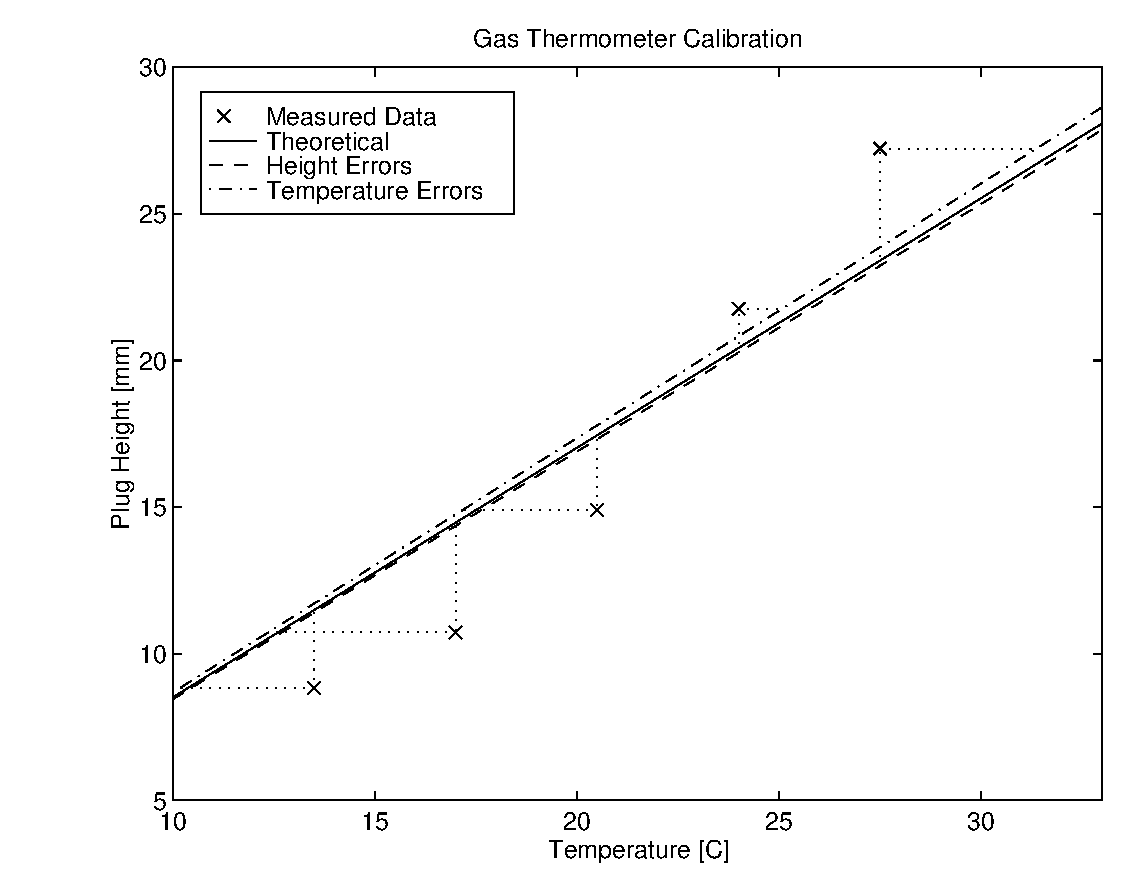
\includegraphics[width=4in]{gastherm.eps}
\end{center}
\caption{Gas Thermometer Example}
\label{gastherm}
\end{figure}

The most well known alternative to least squares is total least squares (TLS).  In TLS we look at the perpendicular distance to the function.  This handles many of the problems of least squares but is more sensitive to errors, as it is ``optimistic'' in how it looks at the problem.  A huge body of literature is dedicated to this problem, and this is the central area of my dissertation (available at www.r2labs.org).  While some of these other methods are very interesting, we will stick to least squares for the moment, but we will remember that problems can occur and so if we have problems we know there are things we can do.

Getting back to business we have a set of $m$ points $(x_{i},y_{i})$ and
a group of $n$ functions $\phi_{i}(x)$ that we want to use to
approximate the points with.  We thus have $m$ equations to find $n$
coefficients.
\beqn
y_{1} & - & \sum_{i=1}^{n}a_{i}\phi_{i}(x_{1}) \\
y_{2} & - & \sum_{i=1}^{n}a_{i}\phi_{i}(x_{2}) \\
& \vdots & \\
y_{m} & - & \sum_{i=1}^{n}a_{i}\phi_{i}(x_{m})
\eeqn
We can rewrite these into a matrix formulation, as
\beqn
Y-\Phi A \\
\eeqn
where
\beqn
Y & = & \left[\begin{matrix}y_{1} & y_{2} & \cdots & y_{m}\end{matrix}\right]^{T} \\
\Phi & = & \left[\begin{matrix}
\phi_{1}(x_{1}) & \phi_{2}(x_{1}) & \cdots & \phi_{n}(x_{1}) \cr
\phi_{1}(x_{2}) & \phi_{2}(x_{2}) & \cdots & \phi_{n}(x_{2}) \cr
\vdots          & \vdots          & \ddots & \vdots \cr
\phi_{1}(x_{m}) & \phi_{2}(x_{m}) & \cdots & \phi_{n}(x_{m})
\end{matrix}\right] \\
A & = & \left[\begin{matrix}a_{1} & a_{2} & \cdots & a_{m}\end{matrix}\right]^{T}.
\eeqn
At this point we want to minimize the square error which is what the
2-norm does, so we have $\min_{A}\| Y-\Phi A\|_{2}^{2}$ .  The norm we
are minimizing is called the
cost function.  The solution is given by $A=\Phi^{\dagger}Y$, where
$\Phi^{\dagger}$ is called the pseudo-inverse of $\Phi$.  Prove it?
Sure!  To avoid getting into some deeper areas of linear algebra we
will assume that $\Phi$ has linearly independent columns.  This is not
restrictive, as we usually have a lot of measurements and only a few
functions we want to fit to them ($m>>n$).

We recall from calculus that the minimum occurs when the gradient (derivative)
is zero. We thus take the gradient of the cost with respect to $A$ and
set it equal to zero to obtain
\beqn
0 & = &
\nabla_{A}\| Y-\Phi A\|_{2}^{2} \\
 & = &
\nabla_{A}(Y-\Phi A)^{T}(Y-\Phi A) \\
 & = &
-\Phi^{T}(Y-\Phi A) \\
 & = &
\Phi^{T}\Phi A-\Phi^{T}Y \\
\Phi^{T}Y
 & = &
\Phi^{T}\Phi A
\eeqn
The last line is what is referred to as the normal equation(s).  Note
that some pluralize it to reflect that the single matrix equation
reflects $n$ scalar equations.  I don't care, use what you like.  We
note that if $\Phi$ has linearly independent columns, then
$(\Phi^{T}\Phi)^{-1}$ exists.
\beqn
\Phi^{T}\Phi A
 & = &
\Phi^{T}Y \\
A
 & = &
(\Phi^{T}\Phi)^{-1}\Phi^{T}Y \\
A
 & = &
\Phi^{\dagger}Y
\eeqn
You might wonder how the last step works.  Some might just call it a definition but in reality it is because $(\Phi^{T}\Phi)^{-1}\Phi^{T}$ satisfies the four conditions of a pseudo inverse (called the Penrose conditions).
\begin{enumerate}
\item $\Phi\Phi^{\dagger}\Phi=\Phi$
\item $\Phi^{\dagger}\Phi\Phi^{\dagger}=\Phi^{\dagger}$
\item $\Phi\Phi^{\dagger}=(\Phi\Phi^{\dagger})^{T}$
\item $\Phi^{\dagger}\Phi=(\Phi^{\dagger}\Phi)^{T}$
\end{enumerate}
The properties are simple and easy to check, and yes, you have to check all four.  Many times a candidate matrix fails only one of them.  The first two properties tell us that it correctly maps the range spaces from the fundamental theorem of linear algebra, and the second two tell us the composite maps are symmetric.  The pseudo-inverse always exists and is unique.  Additionally, when the true inverse exists, it is the pseudo-inverse.  These are just a few of the many reasons to love the pseudo-inverse\ldots

The result is established.  The nice thing about how we have handled things here is we have not specified what the functions are (they have to be linearly independent but that is no problem) or how many of them we want to fit.  You can now fit any combination of functions you like.

The solution is the same for a deterministic assumption, as for an assumption that additive zero mean gaussian noise is present in the measurements, $b$.  The solution can be thought of as the projection of $b$ into the range of $A$, as seen in Figure~\ref{f-geo-ls}.  The cost criterion is appealing to physical intuition, since it requires the solution to account for all of the measurements the system could have produced.  The solution only requires the basic data (system matrix and measurements), and the complexity of the solution is the standard of comparison.  It is easy see why the least squares criterion is popular, but it is not without its problems.  The choice of independent variables, which will be shown below, and scaling problems, which are outlined in \bb{Mendel95}, are few of the well known problems with least squares.
\begin{figure}
\begin{center}
  {\tt    \setlength{\unitlength}{0.92pt}
\begin{picture}(260,185)
\thinlines    \put(69,35){$Ax_{ls}$}
              \put(105,104){$Ax_{ls}-b$}
              \put(164,55){$Ax$}
              \put(86,166){$b$}
              \put(86,163){\line(1,-4){31}}
              \put(12,12){\vector(1,2){75}}
              \put(12,12){\vector(4,1){151}}
              \put(12,12){\vector(0,1){157}}
              \put(13,12){\vector(1,0){237}}
\end{picture}}
\end{center}
\caption{Geometric Interpretation of Least Squares Solution}
\label{f-geo-ls}
\end{figure}

As an example let's look at linear least squares for the points (0,1), (1,2), and (2,3).  We need to find the coefficients $m$, and $b$ for the line.  We construct our matrices
\beqn
Y & = & \left[\begin{matrix}1 & 2 & 3\end{matrix}\right]^{T} \\
\Phi & = & \left[\begin{matrix}
1 & 1 & 1 \cr
0 & 1 & 2
\end{matrix}\right]^{T} \\
A & = & \left[\begin{matrix}b & m\end{matrix}\right]^{T}.
\eeqn

As a second example, consider fitting $e^{ax}$ to (0,1), (1,.5), and
(2,.25).  To separate the coefficient, $a$, from the variable, $x$ we
take the natural log of $y_{i}=e^{ax_{i}}$ to obtain $\ln(y_{i})=ax$.
We can proceed as before now.

As a third example we will consider the second problem where we have
noise (random errors) in the measurements.  These three examples are
coded into Matlab by
\SciLab{Matlab code for examples}{code:LS_example}{scilab/LS_example.m}
and we get the output below and in Fig~\ref{llsqex}.
\begin{list}{}{\leftmargin=3em}\item[]
\begin{verbatim}
A =
    1.0000
    1.0000
ans =
    0
Ae =
   -0.6931
Aee =
   -0.4650
\end{verbatim}
\end{list}

\begin{figure}[h]
\begin{center}
\leavevmode
\hbox{
\epsfxsize=4in
\epsffile{LinLeastSq1.eps}}
\end{center}
\caption{Least Squares Example}
\label{llsqex}
\end{figure}

Homework 8.6: 1,3

\section{Total Least Squares}

\beqn
\min_x\|\bar Ax-\bar b\| \\
s.t.\;
\eeqn

\section{Weighted Least Squares}\label{s-wls}

Weighted least squares is a general technique which seeks to account for the relative importance or accuracy of a row in the equation $Ax-b$ by multiplying by a weighting matrix, which is usually diagonal.  Both row and column weighting can be done \bb{lh95, stew84}, though only the more common case of row weighting will be considered.  Weighted least squares provides a simple way of controlling the influence of a row, although it unfortunately suffers from ill conditioning.  Some major uses of weighted least squares are iterative improvement of a least squares solution \bb{bjorck67, bjorck68, bjorck87, bjgo67, gowi66}, electrical networks, and finite elements \bb{strang88}.  The weighted least squares problem can be stated as
\beqn
\min_{x}\left\|W^{\frac{-1}{2}}(Ax-b)\right\|^{2},
\eeqn
with solution
\beqn
A^{T}W^{-1}Ax &=& A^{T}W^{-1}b \\
x &=& \left(A^{T}W^{-1}A\right)^{-1} A^{T}W^{-1}b.
\eeqn
The main source of ill conditioning is the matrix $W$, which is by its very nature designed to have a large spread in its Eigenvalues.  Vavasis \bb{vav94} claims that this ill condition causes usual techniques for least squares type problems to yield highly inaccurate answers.  Given the ill conditioning, it is reasonable to ask if $x$ ever can become infinite due to $W$.  Both Stewart \bb{stew89} and Todd \bb{todd90} were able to establish independently that for all positive-definite real diagonal matrices, $W$, the following supremums are finite:
\begin{enumerate}
\item
$\sup\left\{\|(A^{T}W^{-1}A)^{-1}A^{T}W^{-1}\|\right\}$
\item
$\sup\left\{\|A(A^{T}W^{-1}A)^{-1}A^{T}W^{-1}\|\right\}$
\end{enumerate}
Since the supremums are finite, $x$ must be finite.   Another question to answer is if a stable method for solution exists.  No method has been shown to be stable using the usual backward error analysis technique, but \bb{hv97} shows one exists  if stability is defined as
\beqn
\|x_{True}-x_{Est}\|\leq\epsilon\cdot f(A)\cdot\|b\|,
\eeqn
where $\epsilon$ is machine precision and $f(A)$ is some function of $A$ that does not depend on $W$.  It is important to note again that a special definition of stability is needed for this problem, due to the conditioning problem in $W$.  The basic solution of \bb{hv97} can then be expressed as

\begin{tabular}{ll}
\hline
    1 & QR factor (with pivoting) $A^{T}W^{\frac{-1}{2}}$: \\
      &    \qquad $A^{T}W^{\frac{-1}{2}} = Q_{1}R_{1}P$ \\
    2 & Reduced QR factor (without pivoting) $R_{1}^{T}$: \\
      &    \qquad $R_{1}^{T}=Q_{2,1}R_{2,1}$ \\
    3 & Solve by back substitution for $z$: \\
      &    \qquad $R_{2,1}z=Q_{2,1}^{T}PW^{\frac{-1}{2}}b$ \\
    4 & Multiply: \\
      &    \qquad $x=Q_{1}z$ \\
\hline
\end{tabular}

The first QR factorization is to provide stabilization.  The second QR factorization is to solve the least squares problem.  The net effect is to factor $A^{T}W^{\frac{-1}{2}}$ into $Q_{1}R_{2,1}^{T}Q_{2,1}^{T}P$, which is essentially a complete orthogonal decomposition \bb{gvl}.

Alternately, the solution can be stated in terms of the equilibrium system
\beqn
\bmat W     & A \\
              A^{T} & 0 \emat
\bmat y \\
              x \emat
=
\bmat b \\
              0 \emat,
\eeqn
and then found by any method desired, such as the QR factorization.  While this has not been shown to be stable, the alternate formulation shows that the weighted least squares problem is essentially a special case of the generalized least squares problem \bb{gvl,paige79a,paige79b,paige85,kp81,benbow99}.

Finally, the weights can be difficult to select if they do not arise naturally.  For instance, in simple DC electrical networks the weights can be considered as resistances, and the $A$ matrix defines the adjacencies, $b$ gives the voltage sources, and $x$ is the desired node voltages.  Such cases naturally give rise to the weights.  What happens when this does not happen?  The engineer is left trying to apply heuristics to select a weighting matrix.  Given the drawbacks, weighted least squares will not be considered further.

\section{Constrained Least Squares}\label{s-cls}

Often constraints naturally arise in problems.  A fitting function could have prescribed values, a physical system could have limits on its operation, or a solution in a particular set could be desired.  Probably the most basic constrained problem is the least squares Quadratic Inequality problem described in \bb{gvl}.  The problem can be stated as
\beqn
  \min_{x}\|Ax-b\| \qquad \hbox{subject to}\qquad \|Bx-d\|\leq\alpha.
\eeqn
Often $d=0$ and $B$ is nonsingular, though this is not required.  The problem can be solved by the method of Lagrange multipliers, which has the nice bonus of having connections to Tikhonov's method, which is dealt with in Section~\ref{s-tik}.  The problem becomes
\beqn
  \min_{x,\lambda}\|Ax-b\|^{2} +\lambda (\|Bx-d\|^{2}-\alpha^{2}).
\eeqn
Taking derivative and setting equal to zero the solution is
\beq
  x & = & (A^{T}A +\lambda B^{T}B)^{-1}(A^{T}b+\lambda B^{T}d) \label{eq-cls-sol} \\
  g(\lambda) & = & \|B(A^{T}A +\lambda B^{T}B)^{-1}(A^{T}b+
             \lambda B^{T}d) - d\|^{2}-\alpha^{2} = 0. \label{eq-cls-sec}
\eeq
Equation~\ref{eq-cls-sol} gives the one parameter family of solutions for the problem.  When the value of the Lagrange multiplier, $\lambda$, is known the unique solution is specified.  Equation~\ref{eq-cls-sec} is called the secular equation in \bb{gvl} and this designation will be used throughout my writings.  The purpose of Equation~\ref{eq-cls-sec} is to find the value of the Lagrange multiplier, $\lambda$.  The multiplier is found by any root finding method desired, though typically Newton's method or bisection is used.  The general procedure of finding a solution to a secular equation by root finding is used in many methods.

A particular case of the least squares quadratic inequality, minimization over a sphere, is of particular importance and has been studied extensively, see \bb{bjorck84, eld77, eld80, eld83, eld84, fg65, gan81, gvl, ols81, scst79, stew84}.  The minimization of a least squares problem over a sphere has strong connections to robustness, and is strongly connected to the Ridge Regression and Cross-validation problems, which will be discussed in Section~\ref{s-rr}.  The basic problem is
\beqn
\min_{\|x\|\leq\alpha}\|Ax-b\|.
\eeqn
Following the procedure outlined above, the solution is found to be
\beqn
x = \left\{
    \begin{matrix} A^{\dagger}b & {\rm if}\qquad\|A^{\dagger}b\|\leq\alpha \\
            (A^{T}A+\lambda I)^{-1}A^{T}b  & {\rm else} \end{matrix} \right..
\eeqn
This special case covers the solution being confined to a particular set, and thus forces the solution to stay bounded.  Since the solution is always bounded to a reasonable size it prevents one problem associated with lack of robustness, namely solutions being unstable and growing without bound.  A major problem with this is how to know a priori the size of the true $\|x\|$.  An error on the guess of the size of $x$ can cause a reduction in the signal strength (as $\|x\|$ is forced to be smaller than the guess).  Another problem is that $\lambda$ can in general be quite large, but experience shows that a small value of $\lambda$ is more desirable as large values tend to remove fine details (usually carried in the singular vectors associated with smaller singular values) first.  The solution obtained from large values of $\lambda$ tend to bear little resemblance to the true solution in all but the major details.  This is a key area of my research, how to get a good value for the regression parameter, $\lambda$ so it neither becomes unstable nor loses data.

\section{Ridge Regression}\label{s-rr}

The Ridge Regression problem is an important special case of constrained least squares.  Ridge Regression can also be considered a special case of Tikhonov regularization, which is covered in Section~\ref{s-tik}.  Golub and Van Loan \bb{gvl} describe the RR problem as
\beq
\min_{x}\| Ax-b\|^{2}+\lambda \|x\|^{2}
\eeq
with the criterion for picking $\lambda >0$ such as $\|x(\lambda)\|\leq\alpha$, i.e. minimization over a sphere as discussed in Section~\ref{s-cls}.

Other techniques for selecting the ridge parameter exist, such as the generalized cross-validation function \bb{ghw79, eld85}.  The cross-validation function seeks to reduce the dependence of the solution on any one experiment, and thus increases the robustness of the problem, as seen in \bb{gvl}.  The cost function for the cross-validation problem is given by
\beqn
C(\lambda) = \frac{1}{m}\sum_{k=1}^{m} w_{k}\left[
  \frac{\bar b_{k} - \sum_{j=1}^{r}u_{kj}\bar
  b_{j}\left(\frac{\sigma_{j}^{2}}{\sigma_{j}^{2}+\lambda}\right)}
  {1 - \sum_{j=1}^{r}u_{kj}^{2}
  \left(\frac{\sigma_{j}^{2}}{\sigma_{j}^{2}+\lambda}\right)}
  \right]^{2}
\eeqn
with
\begin{itemize}
    \item $w_{k}$ a weight on the importance of the $k^{th}$ row (or experiment),
    \item the SVD of $A$ given by $U\Sigma V^{T}$,
    \item $u_{jk}$ is the $j,k^{th}$ element of $U$,
    \item $\sigma_{j}$ is the $j^{th}$ diagonal element of the diagonal matrix $\Sigma$,
    \item and $\bar b=U^{T}b$.
\end{itemize}
Details on the minimization of this cost function are discussed in \bb{ghw79}.  The case of the Ridge Regression problem with the cross-validation function used to select $\lambda$ is often called the cross-validation problem.  No matter how the value of $\lambda$ is selected, the expression for $x(\lambda)$ is given by $x(\lambda)=(A^{T}A+\lambda I)^{-1}A^{T}b$.  It can be easily seen that each component of the RR solution is smaller than the corresponding component of the LS problem, and thus the robustness is gained at the cost of signal strength (or information content).

\section{Tikhonov}\label{s-tik}

The Tikhonov problem can be expressed as
\beq
\min_{x}\| Ax-b\|^{2}+\lambda \|Lx\|^{2}.
\eeq
Note $L$ can be indefinite.  Two parameters can be chosen by the designer to select the desired solution.  The first parameter is $L$, which is used to specify conditions on $x$.  For instance, a solution with a small norm could be desired, which would correspond to picking $L$ to be the identity matrix.  Alternately, a solution with a small derivative could be desired, which corresponds to picking $L$ to be the discrete approximation of the derivative operator.  Similar to weighted least squares, weights could be placed on particular portions of $x$ to limit their sizes.

The second parameter is $\lambda$.  Rather than chose $\lambda$ directly, as is done for $L$, a requirement for $\lambda$ in terms of the rest of the problem is usually chosen.  For instance, the problem of minimizing a solution on a sphere used $\|x(\lambda)\|\leq\alpha$.  What requirement should be used becomes the central discussion of Tikhonov regularization.
\begin{itemize}
\item In \bb{hk70}, it was shown that a non-zero $\lambda$ produces smaller error on average.
\item The discrepancy principle \bb{Mor66} assumes the true system has been corrupted by noise and uses the standard deviation of the noise, to find $\lambda$.
\item The L-curve \bb{Han92} assumes the system is corrupted by noise but does not require as much information on the noise properties as the discrepancy principle.
\item Bounded variations for piecewise continuous functions with at most countably many discontinuities, are handled in \bb{NS98}.
\item Generalized cross-validation \bb{ghw79}, mentioned earlier tries to minimize the dependence on any one trial.
\item Residual and singular value plots have also been suggested \bb{Rust98} to pick $\lambda$.
\item Minimizing the lengths of confidence intervals \bb{PR85} has been done.
\item Even parameter choices for iterative solution methods exist \bb{KOl98}.
\item Most interesting though are the methods that attempt to minimize the distance to the true solution, such as \bb{EG88, Gfr87, HR96, Raus85, OLeary99}.
\end{itemize}

In particular, consider the most recent method as covered in \bb{OLeary99}.  Let the SVD of $A$ be $U\Sigma V^{T}$ and define $\beta=U^{T}b$.  The Tikhonov solution to $Ax\approx b$, with $L=I$ is
\beqn
  x_{tik} & = & V(\Sigma^{T}\Sigma+\lambda I)^{-1}\Sigma^{T}\beta \\
  & = & \sum_{i=1}^{n}\frac{\sigma_{i}\beta_{i}}{\sigma_{i}^{2}+\lambda}v_{i}.
\eeqn
The true system with noise $\epsilon$ can be expressed as
\beqn
  x_{true} & = & V\Sigma^{\dagger}(\beta -\epsilon) \\
  & = & \sum_{i=1}^{n}\frac{\beta_{i}-\epsilon_{i}}{\sigma_{i}}v_{i}.
\eeqn
Minimizing the distance between these two values gives the condition for $\lambda$.  To compute the function exactly requires the knowledge of $\epsilon$, which is not known.  An approximation can be made if the system satisfies the discrete Picard condition (the data values $\beta_{i}-\epsilon_{i}$ goes to zero faster than the singular values) and $\beta_{i}$ is a true value plus noise.  With these assumptions and the standard deviation, $s$, of the noise, the root of the function
\beqn
  \sum_{i=1}^{n}\frac{\beta_{i}^{2}\lambda}{(\sigma_{i}^{2}+\lambda)^{3}}
  -\sum_{i=1}^{k-1}\frac{s^{2}}{(\sigma_{i}^{2}+\lambda)^{2}}
  -\sum_{i=k}^{n}\frac{\beta_{i}^{2}}{(\sigma_{i}^{2}+\lambda)^{2}}
\eeqn
gives the value of $\lambda$.  While the value obtained is an approximation, O'Leary \bb{OLeary99} shows that the resulting $x$ value, $x_{tik}(\lambda)$ is close to the true (using the not approximated value of $\lambda_{true})$ value $x_{tik}(\lambda_{true})$, and that in particular
\beqn
  \frac{\|x_{tik}(\lambda_{true})-x_{tik}(\lambda)\|}{\|x_{tik}(\lambda_{true})\|}
  \leq \frac{|\lambda_{true}-\lambda |}{\sigma_{n}^{2}+\lambda}.
\eeqn
Additionally, as the standard deviation of the noise, $s$, goes to zero, $x_{tik}(\lambda)$ goes to $x_{true}$.  A nice result.  An alternate method of choosing $\lambda$ is presented at the same time using
\beqn
  x_{alt} & = & \sum_{i=1}^{n}\frac{\beta_{i}}{\sigma_{i}+\lambda}v_{i}.
\eeqn
The choice was suggested for Hermitian positive definite matrices \bb{Fran78}, convolution problems with reordering \bb{ER74}, and some additional cases \bb{Han98, Cull80}.  The alternate method proceeds similarly with a small alteration in the function, whose root must be found.  The fact that two methods are suggested, indicates that no one best method exists.  Both perform well however, and demonstrate robustness, which was a major goal.

Tikhonov regularization, works by damping out the terms that correspond to the smaller singular values, see for example \bb{GHO99}.  This can be thought of geometrically as finding a worse model within some bounded region from the original model and solving the LS problem on this new model.  Tikhonov regularization generates robust solutions, but the wealth of techniques to select $\lambda$ shows that there is no obvious best technique.  A drawback to Tikhonov regularization is thus also one of its strengths, namely the wide variety of techniques to pick $\lambda$.  The criterion for picking $\lambda$ is really dependent on the solution desired, for instance, the choice of the solution lying in a ball is usually done to fulfill a heuristic requirement for boundedness.  In the end this method usually ends up being more based on the skill and experience of the engineer who sets up the problem.  This is exactly how the problem is treated in \bb{GHO99, OLeary99}.  The damping of terms corresponding to smaller singular values, essentially means that data and thus accuracy will be lost.  Most of the accuracy loss is due to the ``waterbed effect'', in that accuracy and robustness are competing goals, so advances in one area causes losses in another.  Such competing goals thus are not so much a problem but rather a design decision based on the problem requirements.  The assumptions are another matter.  By adding an implicit heuristic element, the problem de facto includes the ``gut feel'' of the designer.  While this may seem appealing, it is not rigorous, and does not allow for confidence in the final result.  A good guess will give a good result, a bad one a bad result, but there is no way of assessing the guesses.  The desire for a more philosophically pleasing and mathematically rigorous method for posing robust problems led to the development of the min max problem.

\section{Min Max}\label{s-mm}

The min max problem was proposed and solved separately in \bb{cggs} by secular equation techniques and in \bb{GL97} by Linear Matrix Inequality techniques.  This section will concentrate on the secular equation formulation.  The LMI techniques are discussed in Section~\ref{s-lmi}

Simply stated the min max problem seeks to find the worst model in a bounded region, and then solve the problem based on this worst case scenario.  Mathematically it is written as
\beq
\min_{x}\max_{\bmat \|E_A\|\leq\eta \\
                      \|E_{b}\|\leq\eta_{b} \emat }
                      \|(A+E_A)x-(b+E_{b})\|. \label{eq-minmaxorig}
\eeq
This problem can be shown to be equivalent to solving a problem with similar form to the Tikhonov problem, see \bb{cggs}.  Equation~\ref{eq-minmaxorig} can be interpreted geometrically by Figure~\ref{f-geo-min max}.
\begin{figure}
\begin{center}
{\tt    \setlength{\unitlength}{0.92pt}
\begin{picture}(257,204)
\thinlines    \put(93,45){\line(-1,2){10}}
              \put(46,33){\circle{18}}
              \put(14,24){\line(5,3){136}}
              \put(60,69){$\eta\|x\|$}
              \put(175,17){$\|(A+E_{max})x\|$}
              \put(153,100){$\|(A+E_{min})x\|$}
              \put(149,160){$\eta_b$}
              \put(128,176){\line(5,-2){18}}
              \put(130,126){$R$}
              \put(128,176){\circle{38}}
              \put(14,24){\vector(3,4){114}}
              \put(88,7){$(A+E_{max})x_{min\, max}$}
              \put(168,54){$Ax$}
              \put(129,24){\line(0,1){171}}
              \put(92,46){\circle{44}}
              \put(14,24){\vector(4,1){150}}
              \put(14,24){\line(1,0){158}}
              \put(74,124){$b$}
\end{picture}}
\end{center}
\caption{Geometric Interpretation of Min Max Solution}
\label{f-geo-min max}
\end{figure}
The maximization forms the hyperspheres around $A$ and $b$.  The cone around $A$ is formed by varying the size of $x$.  The solution, $x$, and the residual, $R$, are found by connecting the furthest points on the hyperspheres.  The maximization restricts the problem to the lower line of the cone.  The minimization selects the point on the lower cone such that the line segment from the furthest point on the hypersphere around $b$ to the lower cone is perpendicular to the lower cone.  The norm used in \bb{cggs} is the 2-norm, though \bb{gw01} extends it to other norms.  The min max problem becomes
\beq
\min_{x}(\|Ax-b\|+\eta\|x\|+\eta_{b}), \label{eq-minmaxnew}
\eeq
which differs from the typical Tikhonov problem in that the norms are not squared.  As opposed to the Tikhonov problem, the term $\eta$ now has a physical intuition also, that being the amount of uncertainty in the matrix.  Computing the min max solution takes longer than computing the solution to a Tikhonov problem if a simple choice of regression parameter is chosen for the Tikhonov problem, so it is logical to ask why one would want to spend the extra operations to do so.  The simple answer is that the two problems can give arbitrary differences, which we will examine in Section~\ref{s-simdif}.

In the form of Equation~\ref{eq-minmaxnew} it is easy to see that the problem is continuous but non-smooth, since it is non-differentiable whenever $x=0$ or when $Ax=b$.  The solution to Equation~\ref{eq-minmaxnew} and thus Equation~\ref{eq-minmaxorig}, is summarized in Table~\ref{t-min_max}.  For Table~\ref{t-min_max}, let the SVD of $A$ be given by
\beqn
  A = \bmat U_{1} U_{2} \emat
      \bmat \Sigma \\
                    0 \emat V^{T}.
\eeqn
Partition the vector $U^{T}b$ into
\beqn
  \bmat U_{1} U_{2} \emat^{T}b =
  \bmat b_{1} \\
                b_{2} \emat,
\eeqn
and introduce the secular equation
\beqn
  g(\psi) = b_{1}^{T}(\Sigma^{2}-\eta^{2}I)(\Sigma^{2}+\psi I)^{-2}b_{1}
    -\frac{\eta^{2}}{\psi^{2}}\|b_{2}\|^{2},
\eeqn
which has a unique positive root, denoted $\bar\psi$ under the conditions noted in Table~\ref{t-min_max}.  Finally define
\beqn
  \tau_{1}=\frac{\|\Sigma^{-1}b_{1}\|}{\|\Sigma^{-2}b_{1}\|}
  \qquad \hbox{and} \qquad
  \tau_{2}=\frac{\|A^{T}b\|}{\|b\|}.
\eeqn
The solution is thus given below.
\begin{table}[ht]
\begin{center}
\begin{tabular}{l|c|c|}
 & $b\in\Ra(A)$ & $b\not\in\Ra(A)$ \\
\rule{0mm}{1mm} & & \\
\hline
\rule{0mm}{1mm} & & \\
$\eta \ge \tau_{2}$ & 0 & 0 \\
\rule{0mm}{1mm} & & \\
\hline
\rule{0mm}{1mm} & & \\
$\tau_{1} < \eta < \tau_{2}$ & $x = (A^{T}A + \bar\psi I)^{-1}A^{T}b$
   & $x = (A^{T}A + \bar\psi I)^{-1}A^{T}b$ \\
\rule{0mm}{1mm} & & \\
\hline
\rule{0mm}{1mm} & & \\
$\eta \le \tau_{1}$ & $x = A^{\dagger}b$
   & $x = (A^{T}A + \bar\psi I)^{-1}A^{T}b$ \\
\rule{0mm}{1mm} & & \\
\hline
\rule{0mm}{1mm} & & \\
$\eta = \tau_{1} = \tau_{2}$ & $x = \beta A^{\dagger}b$ with $0\le\beta\le 1$
   & $x = (A^{T}A + \bar\psi I)^{-1}A^{T}b$ \\
\rule{0mm}{1mm} & & \\
\hline
\end{tabular}
\end{center}
\caption{Min Max Solution}
\label{t-min_max}
\end{table}
Notice that the least squares solution, $A^{\dagger}b$, is the min max solution under special conditions.  In one case a scaled family of the least squares solution solves the problem.  In general though the solution is given by finding the unique root of the secular equation, $g(\psi)$ in the positive quadrant.  When $\eta$ is large the solution is zero.

\section{Comparison of Min Max and Tikhonov}\label{s-simdif}

At this point, it is reasonable to ask if there is a similar, but simpler way to solve the problem, which exhibits the desired behavior of min max that can be solved instead of the min max methodology of \bb{cggs,gw01,GL97}.  One candidate solution that has been suggested is Tikhonov regulation.  It has a large body of literature, such as \bb{GHO99, OLeary99}, and a closed form solution.  Start by noting that a reasonable choice for the parameter $\lambda$ in the Tikhonov problem is to chose it to be equal to the square of the uncertainty, since all the other terms are squared and this will account for the size of the uncertainty.  In this case the model has a closed form solution which is given by
\beq
\hat x = \left( A^{T}A + \eta^{2}I\right)^{-1}A^{T}b.
\eeq
Note that this is clearly a regularized estimator, with the regularization parameter given by the bound in the error. Note also that for the min max problem that if $Ax\neq b$ and $x\neq 0$ then the min max problem also has a solution with a similar form given by
\beq
\hat x & = & \left( A^{T}A + \alpha I\right)^{-1}A^{T}b \\
\alpha & = & \eta\frac{\left\| Ax-b\right\|}{\left\| x\right\|}.
\eeq
The min max problem is also a regularized solution, with the regularization parameter given by $\alpha$.  Since $\alpha$ is dependent on unknown values it must be calculated, which is usually done by a secular equation.  The logical question is, ``Why not use the Tikhonov cost function, which has the closed form solution?''  To answer this it must be seen if the Tikhonov problem's regularization parameter can be arbitrarily larger or smaller.  If the Tikhonov problem's parameter can be arbitrarily larger, then the solution can be over regularized and thus valuable information can be lost.  If the Tikhonov parameter can be arbitrarily smaller, then the solution can be under regularized and thus the solution might not be robust.  Thus to compare the two, examine the ratio of the min max problem's regularization parameter, $\alpha$, to the Tikhonov problem's regularization parameter, $\eta^{2}$.  Doing so, obtain
\beq
\frac{\alpha}{\eta^{2}} & = & \frac{\left\| Ax_{mm}-b\right\| }{
    \eta\left\| x_{mm}\right\|}.
\eeq

\subsection{Over-Regularization}

First, see if the Tikhonov problem can be over regularized, which is the more dangerous problem.  This corresponds to the ratio being arbitrarily small.  Note that $\| Ax_{mm}-b\|\leq\| b\|$ at the solution, by noting the cost at the solution must be less than the cost at the point $x=0$.  Thus,
\beq
\frac{\alpha}{\eta^{2}} & \leq &
     \frac{\left\| b\right\| }{ \eta\left\| x_{mm}\right\|}.
\eeq
It is clearly possible to pick $A$ and $b$ such that $\eta\| x_{mm}\| \gg \| b\|$.  For example consider the following simple system,
\beq
A=\bmat 0.2 \\
                0 \emat \qquad
b=\bmat 5 \\
                1 \emat \qquad
\eta =0.1.
\eeq
For this simple system the min max problem has a solution of $x_{mm}=22.11$ while the modified problem has a solution of $x_{T}=20$.  We note that for this problem the Tikhonov regularization parameter is twice as large as the min max problem.  Clearly the over-regularization has also yielded a loss of information that is not warranted by the problem.  We note that while this simple example does not show an arbitrarily large ratio difference, since it is used only as a numerical motivation.  To see the arbitrary difference consider the following for $\delta \ll 1$,
\beq
A=\bmat \delta \\
                0 \emat \qquad
b=\bmat \frac{1}{\delta} \\
                \delta \emat \qquad
\eta =\frac{\delta}{ 2}.
\eeq
For this system note that the least squares (LS) solution is given by $x_{LS}=\frac{1}{\delta^{2}}$, and the min max system is $x_{mm}=\frac{1}{\delta^{2}}-\frac{1}{\delta\sqrt{3}}$.  Note that since $\delta \ll 1$, the min max estimate is extremely close to the LS solution.  The Tikhonov problem solution is given by $x_{T}=\frac{4}{5\delta^{2}}$, which is easily seen to be arbitrarily far from the desired solution, since for $\delta \ll 1$ the two candidate solutions differ by almost $20\%$ of an arbitrarily large number.  Moreover, the ratio of regularization parameters is approximately given by the arbitrarily small number,
\beq
\frac{\alpha}{\eta^{2}} & \approx & \frac{4 }{ \sqrt{3}}\delta^{2}.
\eeq

\subsection{Under-Regularization}

The second area to be considered is if the Tikhonov problem can be under-regularized.  This corresponds to the ratio of $\alpha$ over $\eta^{2}$ being arbitrarily large.  Note that $\| Ax_{mm}-b\|\geq\| P_{A^{\perp}}b\|$, thus
\beq
\frac{\alpha}{\eta^{2}} & \geq &
   \frac{\left\| P_{A^{\perp}} b\right\| }{ \eta\left\| x_{mm}\right\|}.
\eeq
It is clearly possible to pick $A$ and $b$ such that $\| x_{mm}\| \ll \| P_{A^{\perp}}b\|$.  For example consider the following simple system,
\beq
A=\bmat 1 \\
                0 \emat \qquad
b=\bmat 1 \\
                1  \emat \qquad
\eta=1.
\eeq
Note that since the perturbation is as large as the norm of the $A$ matrix, $x_{mm}=0$, which corresponds to $\alpha \rightarrow \infty$.  This is intuitively pleasing, as it confirms the belief that no valid information exists for a system with uncertainty as large as the system.  Note also that $x_{LS}=1$.  Now the Tikhonov problem has the solution $x_{T}=\frac{1}{ 2}$.  Not only is this clearly too optimistic an answer, it is also unrealistic.  The ratio is infinite and thus arbitrarily large, as was desired to be shown.  Thus while the Tikhonov problem has nice properties for calculation, its estimator can be arbitrarily different than the min max problem.  Additionally, the Tikhonov problem does not correspond to physical intuition as can be seen in the last example above.  The min max problem can thus not be altered to an apparently similar problem and solved for that system.

\section{Non-Degenerate Min Min}\label{s-ndmm}

The non-degenerate min min problem was presented in \bb{cgs99} for the
case of the 2-norm and extended to other norms in \bb{gw01}.  The
essential idea is to assume, similar to total least squares, that the
actual system $A+E_A$ and $b+E_{b}$ is such that $b+E_{b}$ is as close
to being in the subspace defined by $A+E_A$ as possible.  The residual is
then minimized over all choices $x$.  The problem is thus expressed as
\beq
\min_{x}\min_{\bmat \|E\|\leq\eta \\
                      \|E_{b}\|\leq\eta_{b} \emat }
                      \|(A+E_A)x-(b+E_{b})\|. \label{eq-minminorig}
\eeq
The geometric view is very similar to the min max problem and is
provided in Figure~\ref{f-geo-minmin}.  The cone around $A$ and the
ball around $b$ are the same as before (i.e.: all possible values for
the problem).  The min min problem is thus to find the smallest
distance from the ball to the cone, which is shown in the figure.
Note that it is possible for the ball and cone to have points in
common, this is the degenerate case, and is covered in Chapter~\ref{c-degmm}.
\begin{figure}
\begin{center}
{\tt    \setlength{\unitlength}{0.92pt}
\begin{picture}(257,162)
\thinlines    \put(90,39){\line(5,-2){21}}
              \put(44,27){\circle{18}}
              \put(12,18){\line(1,0){158}}
              \put(12,18){\vector(4,1){150}}
              \put(12,18){\line(5,3){134}}
              \put(90,39){\circle{44}}
              \put(168,49){$A$}
              \put(105,64){$x$}
              \put(88,120){\circle{36}}
              \put(107,92){$R$}
              \put(82,143){$\eta_b$}
              \put(153,95){$\|(A+E_{min})x\|$}
              \put(175,12){$\|(A+E_{max})x\|$}
              \put(110,25){$\eta\|x\|$}
              \put(88,120){\line(0,1){17}}
              \put(94,81){\line(1,-2){6}}
              \put(94,81){\line(5,3){11}}
\thicklines   \put(97,103){\line(1,-2){13}}
\thinlines    \put(12,18){\vector(3,4){76}}
              \put(51,85){$b$}
\end{picture}}
\end{center}
\caption{Geometric Interpretation of Min Min Solution}
\label{f-geo-minmin}
\end{figure}
This section will cover the non-degenerate condition.  Two main
issues are:
\ben
\item find a computable condition for checking degeneracy,
\item find a secular equation and region to find the solution.
\een

First, find a computable condition for degeneracy.  For the problem to be
non-degenerate the residual must be greater than the possible
perturbation.  In equation form this is
\beq
\eta\|x\|<\|Ax-b\|. \label{eq-degen-ndmm}
\eeq
This equation depends on the solution, $x$, so an equation with only
$A$, $b$, and $\eta$ is desired.  By squaring the degeneracy
condition, Equation~\ref{eq-degen-ndmm}, the condition becomes
\beq
x^{T}(A^{T}A-\eta^{2}I)x-2x^{T}A^{T}b+b^{T}b>0. \label{eq-quad-ndmm}
\eeq
For this to hold for all $x$, the minimum value of the function must
be greater than zero.  The function must have a finite minimum, and
that minimum must be positive.  To have a finite minimum, the
following must hold
\beqn
A^{T}A-\eta^{2}I>0,
\eeqn
or defining the minimum singular value of $A$ to be $\sigma_{min}$,
\beq
\sigma_{min}>\eta. \label{eq-small-ndmm}
\eeq
Noting that in practice $\eta>0$ ($\eta=0$ is least squares), this requires
that $A$ is full rank, which is assumed from now on.  Provided
Equation~\ref{eq-small-ndmm} holds, the minimum value of
Equation~\ref{eq-quad-ndmm} is
\beq
b^{T}\left[I-A(A^{T}A-\eta^{2}I)^{-1}A^{T}\right]b>0. \label{eq-close-ndmm}
\eeq
The problem is non-degenerate if $A$ is full rank, and both
Equation~\ref{eq-small-ndmm} and Equation~\ref{eq-close-ndmm} hold.

The computable condition is needed to see if the non-degenerate
case applies (if it doesn't the non-degenerate case of
Chapter~\ref{c-degmm} holds) and is useful in the proof.  The proof of the solution is too
lengthy to present here, readers are referred to \bb{cgs99} for a full
treatment.  Assume the problem is non-degenerate and let the SVD of
$A$ be
\beqn
A=\bmat U_{1} & U_{2} \emat
  \bmat \Sigma \\
                0 \emat V^{T},
\eeqn
with smallest singular value $\sigma_{n}$ and corresponding left
singular vector $u_{n}$.
Define
\beqn
\bmat b_{1} \\
              b_{2} \emat
=\bmat U_{1} & U_{2} \emat^{T}b.
\eeqn
Then for the secular equation,
\beqn
g(\psi) = b_{1}^{T}(\Sigma^{2}-\eta^{2}I)(\Sigma^{2}-\psi
I)^{-2}b_{1}-\frac{\eta^{2}}{\psi^{2}}\|b_{2}\|^{2},
\eeqn
find the unique root of $g(\psi)$ in the interval
$(\eta^{2},\sigma_{n}^{2})$ and if it exists call it $\hat\psi$,
otherwise let $\hat\psi=\sigma_{n}^{2}$.  If
$\hat\psi<\sigma_{n}^{2}$ then the solution is
\beqn
x=(A^{T}A-\hat\psi I)^{-1}A^{T}b,
\eeqn
else there are two solutions
\beqn
x & = & V\bmat
    (\bar\Sigma^{2}-\sigma_{n}^{2}I)^{-1}\bar\Sigma\bar b_{1} \\
    \pm\frac{\sigma_{n}}{\sqrt{\sigma_{n}^{2}-\eta^{2}}}\sqrt{-\bar g(\sigma_{n}^{2})
    } \emat
\eeqn
with
\beqn
\bar g(\psi) & = &
  g(\psi)-(u_{n}^{T}b)^{2}
  \frac{\sigma_{n}^{2}-\eta^{2}}{(\sigma_{n}^{2}-\psi)^{2}} \\
\Sigma & = &
  \bmat
  \bar\Sigma & 0 \\
  0 & \sigma_{n}
   \emat \\
b_{1} & = &
  \bmat
  \bar b_{1} \\
  b_{1,n}
   \emat
   =
  \bmat
  \bar b_{1} \\
  0
   \emat. \\
\eeqn
My dissertation completed the analysis of this problem
by solving the degenerate case, which turns out to be the more general
situation.

\section{LMI Techniques}\label{s-lmi}

Of all the techniques presented the Linear Matrix Inequality (LMI) techniques are the most
flexible.  Most of the techniques both currently used can be solved using LMI techniques.  The Backward Error
method is an example of a problem that does not fit into the LMI
framework, due to its rational cost function.  The principle concern
of this section is to consider the LMI techniques that are similar to
what is covered in my dissertation.  In \bb{BV02,BL02,EgG01,GL97,LB97,LVBL98,LB01}, the LMI
methodology for solving the min max problem with and without structure
were covered.  This section will cover two principle areas of \bb{GL97},
that being the structured and unstructured case.

The unstructured perturbations are identical to the min max case.  The
problem is defined as
\beqn
\min_{x}\max_{\|E E_{b}\|_{F}\leq 1}\|(A+E_A)x-(b+E_{b})\|.
\eeqn
Note that the bound is $1$ since the problem can always be normalized
to this by dividing $A$ and $b$ by any other bound thus yielding a
problem of the form above.  The problem can be reformulated as a  Second-Order Cone Programming (SOCP) problem
of the form
\beqn
&& \min\lambda \\
&& \qquad s.t.\qquad \bmat \|Ax-b\|\leq \lambda-\tau \\
                          \left\|\bmat x \\
                                               1 \emat\right\|
                             \leq\tau \emat .
\eeqn
Define $\psi$ to be $\frac{(\lambda -\tau)}{\tau}$.  The solution can
then be shown to be
\beqn
x=\left\{\bmat (A^{T}A+\psi I)^{-1}A^{T}b & \text{if}\; \psi>0 \\
                A^\dagger b & \text{else} \emat
\right.
\eeqn
with $\lambda$ and $\tau$ are the unique optimal points for the system.  The parameter $\psi$ is the same as was found in the min max problem by secular equation techniques.

At this point it is reasonable to ask why further work should be done.  The basic reason is speed. Each iteration of a SOCP is basically $O((m+n)n^{2})$ and \bb{GL97} asserts that the number of iterations is almost constant and independent of the problem size, resulting in a reasonably sized constant multiplying the $n^{3}$.  In contrast, solving a secular equation can be done in iterations that are $n^{2}$ and then the overall solution takes $n^{3}$ but has a smaller constant since it mostly comes from the calculation of the SVD (the ``light'' version of the SVD can be used further saving time). In \bb{GL97}, it is noted that both have the same order of complexity, which is true, but order is not the only determiner, the constant that is ignored when reporting order can greatly influence practical speed.  The speed advantage of secular techniques is noted in \bb{GL97},  thus secular equation techniques have a slight advantage over SOCP.  In \bb{LVBL98} it is asserted that the secular equation technique is simpler and that LMI techniques only have advantage over secular techniques on robust regression problems when additional constraints need to be applied.  Noting that SOCP problems can be solved faster than SDP (semi-definite programming) problems, the use of secular equation techniques becomes more apparent.  On a different line, developing algorithms to solve problems in different ways is a valuable goal in and of itself, that yields benefits in many areas from theoretical understanding to programming implementations.  The nice features of the LMI techniques thus do not rule out the other solution techniques, rather they complement each other and serve to give a more complete understanding.

The second area to cover is the structured perturbations problem.  The structured perturbations can approximate the multi-column, multi-row, and general min max problems developed in my dissertation and some cases not expressible in one of the proposed techniques.  Note that the structured case can approximate but not directly solve the cases covered in my dissertation.  The structured perturbations are of the form
\beqn
E(\delta_{1},\ldots,\delta_{p}) & = & \sum_{k=1}^{p}\delta_{k}E_{k} \\
E_{b}(\delta_{1},\ldots,\delta_{p}) & = & \sum_{k=1}^{p}\delta_{k}E_{b,k}
\eeqn
where $p$ is the number of basic perturbations, and $E_{k}$ is a fixed basic perturbation on $A$ and $E_{b,k}$ is a fixed basic perturbation on $b$.  The problem with trying to directly solve the multi-column case (for instance) is that the basic perturbations would need to be,
\beqn
E_{1} & = & \frac{Ax-b}{\|Ax-b\|}
 \frac{\bmat x_{1}^{T} & 0 & \ldots & 0 \emat}{\|x_{1}\|} \\
 & \vdots & \\
E_{p} & = & \frac{Ax-b}{\|Ax-b\|}
 \frac{\bmat 0 & \ldots & 0 & x_{p}^{T} \emat}{\|x_{p}\|}.
\eeqn
This requires $E_{k}$ to be dependent on $x$ and thus the LMI to solve the problem that is presented, is no longer linear.  The multiple column case is used in \bb{GL97} as a motivation for the linear-fractional case, which is shown to be NP-hard in the general case and for which an upper bound for the worst case residual was obtained.  As special cases, the multiple column, multiple row, and general block perturbation cases are not NP-hard, and allow for the results in my dissertation.  The three cases could be approximated with the structured problem (as opposed to the linear-fractional) by examining a series of problems with the values of $E_{k}$ based off the previous problem's solution, starting with say $x=A^{\dagger}b$, though it is not obvious if this would converge.  Optionally the problem could be approximated by some other column (row, or general also) structure, though it will not necessarily generate the same one found in my dissertation.  Undoubtedly an LMI formulation can be found to solve the same problem, the key point is that the structured formulation as outlined in \bb{GL97} will not.  The formulation in \bb{GL97} does permit important structures, such as Toeplitz, that cannot be handled in the formulations of my dissertation.  Each formulation is useful and has a place, the needs of each  individual problem under consideration determine which to use.
%%%%%%%%%%%%%%%%%%%%%%%%%%%%%%%%%%%%%%%%%%%%%%%%%%%%%%%%%%%%%%%%%%%%%
Returning to the structured problem, first define the following:
\beqn
M & = & \bmat
           E_{1}x-E_{b,1} & \ldots & E_{p}x-E_{b,p} \emat \\
F & = & M^{T}M \\
g & = & M^{T}(Ax-b) \\
h & = & \|Ax-b\|.
\eeqn
The problem can be written as
\beqn
\min_{x}\max_{\|\delta\|\leq1}
\bmat 1 \\
              \delta \emat^{T}
\bmat h & g^{T} \\
              g & F \emat
\bmat 1 \\
              \delta \emat.
\eeqn
The problem can then be solved by the SDP,
\beqn
& & \min\lambda \\
& & \qquad s.t.\qquad \bmat \lambda-\tau & 0 & (Ax-b)^{T} \\
                                    0 & \tau I & M^{T} \\
                                    Ax-b & M & I \emat\geq 0.
\eeqn
The SDP formulation, while not as efficient as a SOCP formulation, is
still polynomial time, and can be solved by interior point algorithms.
The variety of structures that can be handled or approximated by the
structured technique in \bb{GL97} is tremendous and covers most of
the cases of interest.  Problems still exist which cannot be directly
handled, or which could be solved more efficiently by specialized
solvers.

\section{Simple Comparative Example}

The previous discussion includes three general groups of problem formulations that can be used in estimation.  The following provides a feel for how these problems operate on a simple example.  Consider a simple one dimensional ``skyline'' image that has been blurred.  A ``skyline'' image is a one dimensional image that looks like a city skyline when graphed, and thus is the most basic image processing example.  ``Skyline'' images involve sharp corners, and it is of key importance to accurately locate these corner transitions.  Blurring occurs often in images, for example atmospheric conditions, dust or imperfections in the optics can cause a blurred image.  Blurring is usually modelled as a gaussian blur, which is a smoothing filter.  The gaussian blur causes greater distortion on the corners, which is exactly where we do not want it.  The component of a gaussian blur with standard deviation, $\sigma$, in position, ($i$,$j$), is given by
\beqn
G_{i,j} = e^{-\left(\frac{i-j}{\sigma}\right)^{2}}.
\eeqn
Going on the presumption that the exact blur that was applied is not known ($\sigma$ unknown) the exact system cannot be recovered.  While the original system cannot be perfectly extracted, some improvement on the blurred image is desirable.  The blur is ``known'' to be small compared to the information so some improvement should be possible.
\begin{figure}
\begin{center}
\leavevmode
\hbox{%
\epsfxsize=5.5in
\epsffile{skyline.eps}}
\end{center}
\caption{Skyline Problem}
\label{skyline}
\end{figure}
The least squares solution fails completely, yielding a
result that is about three orders of magnitude off in the scale and is oscillating badly, see
Figure~\ref{skyline}.  Notice that the total least squares solution
is better than the least squares solution (only off by an order of magnitude and the oscillations are slower), but still not acceptable.  The
Tikhonov solution works well due to its increased robustness.  All of the methods of my dissertation can be seen to
yield very good solutions to the problem.




\chapter{Solving Systems of Linear Equations}



\section{Solving Triangular Systems}
We will begin our solution of general linear equations by considering how to solve triangular systems.  This simpler form of system is particularly easy to solve, and it is easy to make other systems become triangular.  In later sections reducing a matrix to triangular form becomes a standard tool.

As a side note, we really don't like reducing to a triangular matrix.  It is better to reduce to upper or lower Hessenberg form\footnote{triangular plus one non-zero diagonal immediately past the main diagonal}.  Similarly, real numerical systems often avoid diagonalizing and reduce to tridiagonal matrix\footnote{The only non-zero elements are on the main diagonal and the diagonals immediately next to it}.  The reason is it is often difficult to zero the elements right next to the main diagonal, so we often get most of the way and then finish the job with an iterative method.  Starting with an iterative method would be slow.  This way we get the best of both systems.

\subsection{Forward Substitution}

Consider a system $Lx=b$, where $L$ is a square lower triangular matrix.
\begin{eqnarray}
\left[\begin{matrix}
l_{1,1} & 0       & \cdots & 0 \\
l_{2,1} & l_{2,2} & \ddots & \vdots \\
\vdots  & \vdots  & \ddots & 0 \\
l_{n,1} & l_{n,2} & \cdots & l_{n,n}
\end{matrix}\right]
\left[\begin{matrix}
x_1 \\
x_2 \\
\vdots \\
x_n
\end{matrix}\right]
&=&
\left[\begin{matrix}
b_1 \\
b_2 \\
\vdots \\
b_n
\end{matrix}\right] \label{eq-lowertriangluarLS}
\end{eqnarray}
The first row tells us
\begin{eqnarray}
l_{1,1}x_1 &=& b_1 \nonumber \\
x_1 &=& \frac{b_1}{l_{1,1}} \label{eq-lowertriangluarLS-row1}
\end{eqnarray}
Using the solution of the first line and the equation of the second row we find
\begin{eqnarray}
l_{2,1}x_1 + l_{2,2}x_2 &=& b_2 \nonumber \\
x_2 &=& \frac{b_2-l_{2,1}x_1}{l_{2,2}} \\
x_2 &=& \frac{b_2-l_{2,1}\frac{b_1}{l_{1,1}}}{l_{2,2}} \nonumber
\end{eqnarray}
In essence we are removing the effect of $x_1$ on $b$ and then solving just as we did in Eq~\ref{eq-lowertriangluarLS-row1}.  With the knowledge of $x_2$ we will need to remove its effect on $b$ for subsequent calculations.  We can generalize this into a simple procedure.  The one thing we have to make sure is that the elements on the main diagonal never become zero\footnote{There are a lot of ways of explaining why this is from the matrix itself, here are a two.  For lower (or upper) triangular systems the determinant is the product of the diagonal elements, thus if one is zero then the determinant is zero and no inverse exists.  A zero on the diagonal of a triangular (upper or lower) matrix means there is a zero eigenvalue, and hence the matrix is not invertible.}, as we need to divide by them.
\SciLab{SciLab code for forward substitution}{cod-forward-substitution}{scilab/forward_substitution.sci}
Listing~\ref{cod-forward-substitution} shows SciLab code for a forward substitution function.  Note that it has complexity $\frac{n^2}{2}$, which is much better than the $n^3$ for matrix inversion.  In Listing~\ref{cod-forward-substitution-test}, is SciLab code that uses the forward substitution function.  The exec command causes SciLab to run the contents of the file containing forward\_substitution, thus defining it for use on the next line.
\SciLab{SciLab test code for forward substitution}{cod-forward-substitution-test}{scilab/forward_substitution_test.sce}

\subsection{Backward Substitution}

Now consider a system $Ux=b$, where $U$ is a square upper triangular matrix.
\begin{eqnarray}
\left[\begin{matrix}
u_{1,1} & u_{1,2} & \cdots & u_{1,n} \\
0       & u_{2,2} & \cdots & u_{2,n} \\
\vdots  & \ddots  & \ddots & \vdots \\
0       & \cdots  & 0      & u_{n,n}
\end{matrix}\right]
\left[\begin{matrix}
x_1 \\
x_2 \\
\vdots \\
x_n
\end{matrix}\right]
&=&
\left[\begin{matrix}
b_1 \\
b_2 \\
\vdots \\
b_n
\end{matrix}\right] \label{eq-uppertriangluarLS}
\end{eqnarray}
The last row tells us
\begin{eqnarray}
u_{n,n}x_n &=& b_n \nonumber \\
x_n &=& \frac{b_n}{u_{n,n}} \label{eq-uppertriangluarLS-row1}
\end{eqnarray}
Using the solution of the last line and the equation of the second to last row we find
\begin{eqnarray}
u_{n-1,n}x_n + u_{n-1,n-1}x_{n-1} &=& b_{n-1} \nonumber \\
x_{n-1} &=& \frac{b_{n-1}-u_{n-1,n}x_n}{u_{n-1,n-1}} \\
x_{n-1} &=& \frac{b_{n-1}-u_{n-1,n}\frac{b_n}{u_{n,n}}}{u_{n-1,n-1}} \nonumber
\end{eqnarray}
In essence we are removing the effect of $x_n$ on $b$ and then solving just as we did in Eq~\ref{eq-uppertriangluarLS-row1}.  With the knowledge of $x_{n-1}$ we will need to remove its effect on $b$ for subsequent calculations.  We can generalize this into a simple procedure.  As in the lower triangular matrix of the forward substitution case, the one thing we have to make sure is that the elements on the main diagonal never become zero\footnote{There are a lot of ways of explaining why this is from the matrix itself, here are a two.  For lower (or upper) triangular systems the determinant is the product of the diagonal elements, thus if one is zero then the determinant is zero and no inverse exists.  A zero on the diagonal of a triangular (upper or lower) matrix means there is a zero eigenvalue, and hence the matrix is not invertible.}, as we need to divide by them.
\SciLab{SciLab code for backward substitution}{cod-backward-substitution}{scilab/backward_substitution.sci}
Listing~\ref{cod-backward-substitution} shows SciLab code for a backward substitution function.  Note that it has complexity $\frac{n^2}{2}$, which is much better than the $n^3$ for matrix inversion.  In Listing~\ref{cod-backward-substitution-test}, is SciLab code that uses the backward substitution function.  The exec command causes SciLab to run the contents of the file containing backward\_substitution, thus defining it for use on the next line.
\SciLab{SciLab test code for backward substitution}{cod-backward-substitution-test}{scilab/backward_substitution_test.sce}

\section{LU Factorization}

Since we have ways to solve a system of matrices, $Ax=b$, where $A$ is either upper or lower triangular, it makes sense to ask can we transform any matrix into this form and then solve it.  It turns out we can, and it is fairly fast, but not numerically stable\footnote{Basically this means it can give very wrong answers under certain circumstances.  Don't do this with badly conditioned matrices unless you really know what you are doing.}.  First I provide code in Listing~\ref{cod-lu_no_pivot} to find both $L$ (a lower triangular matrix) and $U$ (an upper triangular matrix), such that $LU=A$.  Theoretically you could use this and your forward and backward solver to get the solution.  In practice we don't do this for two reasons.  First, it cannot handle a zero value on the main diagonal (row $=$ col), which will be handled by pivoting.  Second, though is that we don't need to know $L$, we just need $U$ and $L^{-1}b$.  This can be seen by the following
\begin{eqnarray}
Ax &=& b \\
LUx &=& b
\end{eqnarray}
Note that this step is seen simply by noting $A=LU$ by construction of $L$ and $U$.
\begin{eqnarray}
LUx &=& b \\
L^{-1}LUx &=& L^{-1}b \\
Ux &=& L^{-1}b
\end{eqnarray}
The next step is the basic algebraic rule of multiplying both sides by the same thing does not change them.  The last step combines the definition of an inverse, namely $L^{-1}L=I$, and the property of $I$ that $IU=U$.  Thus to find $x$ we need $U$ and $L^{-1}b$.  The code for this is in Listing~\ref{cod-lusolver_no_pivot}.  Note you could also just write a function that returns $U$ given $A$, and then pass $\left[\begin{matrix}A & b\end{matrix}\right]$ instead of just $A$, and your function will return $\left[\begin{matrix}U & L^{-1}b\end{matrix}\right]$.

\SciLab{Gaussian Elimination (LU factorization)}{cod-lu_no_pivot}{scilab/lu_no_pivot.sci}
\SciLab{Solving $Ax=b$ using LU factorization}{cod-lusolver_no_pivot}{scilab/lusolver_no_pivot.sci}

\subsection{Partial Pivoting}

\SciLab{Gaussian Elimination with row pivoting (LU factorization with partial pivoting)}{cod-lu_partial_pivot}{scilab/lu_partial_pivot.sci}

\subsection{Cholesky Factorization}

For symmetric ($A=A^T$), positive definite ($x^TAx>0\;\forall x\neq 0$) we can perform a special form of the LU factorization called the Cholesky factorization ($A=LL^T$).  To see how this works consider the following
\begin{eqnarray*}
L &=& \left[\begin{matrix}
l_{1,1} & 0       & \cdots & 0 \\
l_{2,1} & l_{2,2} & \ddots & \vdots \\
\vdots  & \vdots  & \ddots & 0 \\
l_{n,1} & l_{n,2} & \cdots & l_{n,n}
\end{matrix}\right] \\
LL^T &=&\left[\begin{matrix}
l_{1,1} & 0       & \cdots & 0 \\
l_{2,1} & l_{2,2} & \ddots & \vdots \\
\vdots  & \vdots  & \ddots & 0 \\
l_{n,1} & l_{n,2} & \cdots & l_{n,n}
\end{matrix}\right]\left[\begin{matrix}
l_{1,1} & l_{2,1} & \cdots & l_{n,1} \\
0       & l_{2,2} & \cdots & l_{n,2} \\
\vdots  & \ddots  & \ddots & \vdots \\
0       & \cdots  & 0      & l_{n,n}
\end{matrix}\right] \\
&=& \left[\begin{matrix}
l_{1,1}^2      & l_{1,1}l_{2,1}      & \cdots & l_{1,1}l_{n,1} \\
l_{2,1}l_{1,1} & l_{2,2}^2+l_{2,1}^2 & \ddots & \vdots \\
\vdots         & \ddots              & \ddots & l_{n,n-1}l_{n-1,n-1}+\sum_{i=1}^{n-2}l_{n,i}l_{i,n-1} \\
l_{n,1}l_{1,1} & \cdots              & l_{n,n-1}l_{n-1,n-1}+\sum_{i=1}^{n-2}l_{n,i}l_{i,n-1} & l_{n,n}^2+\sum_{i=1}^{n-1}l_{n,i}^2
\end{matrix}\right]
\end{eqnarray*}


\SciLab{Cholesky Factorization}{cod-cholesky}{scilab/Cholesky.sci}

\section{QR Factorization}

While in most practical systems LU or a specialized version like Cholesky will work nicely, there are times when numerical conditioning makes these methods dangerous.  This is when we can use a more numerically savvy routine, QR factorization.  The idea of QR factorization is to obtain an upper triangular matrix, $R$, similar to LU, but to do it with orthogonal transformations. Orthogonal transforms use orthogonal matrices, which have a variety of nice properties
\begin{enumerate}
  \item The inverse is the transpose ($Q^{-1}=Q^T$)
  \item The norm is 1 ($\|Q\|=1$)
  \item The norm of the inverse is 1 ($\|Q^{-1}\|=\|Q^T\|=\|Q\|=1$)
  \item The condition number is 1 ($cond(Q)=\|Q\|\|Q^{-1}\|=1$)
\end{enumerate}
The first and last property are particulary nice for us.  Since the condition number is 1, we should not cause any errors to grow.  Since the transpose is the inverse it is easy and relatively quick to calculate.  There are several ways to do QR, which revolve around how to form $Q$ or $R$.  To understand these methods, you first need to understand basis, dimensionality of vector spaces, and orthogonality, but those in turn requires an understanding of independence.  If you are not familiar with any of these concepts please read Section~\ref{s-basis}.

\subsection{Gram-Schmidt Orthogonalization}
This is the easiest to understand, but the worst to do.
\SciLab{Classic Gram-Schmidt Orthogonalization}{cod-gramschmidt_classic}{scilab/gram_schmidt_classic.sci}

\subsection{Modified Gram-Schmidt Orthogonalization}
The fix gains some precision but does not fix the root problem.
\SciLab{Modified Gram-Schmidt Orthogonalization}{cod-gramschmidt_modified}{scilab/gram_schmidt_modified.sci}

\subsection{Givens Rotations}
This works well, and is best suited to sparse matrix solvers because it can be used to target individual, non-zero elements without effecting other terms.  Each Givens rotation only effects only two rows or columns in the target matrix (depends on if you do left or right multiplication). A rotation matrix is given by
\begin{eqnarray}
R_{\theta} &=& \left[\begin{matrix}\cos\theta & -\sin\theta\\
                                   \sin\theta & \cos\theta\end{matrix}\right].
\end{eqnarray}
Givens rotations are the 4 elements of a rotation matrix in a square pattern centered on the diagonal.  Being rotations they are very nice to calculate, easy to express, but have a higher overhead to do them for every non-zero term.  When there are only a few non-zero terms (i.e. sparse matrices) this is not bad, and they end up being much more efficient than other methods that will calculate how to zero a zero element.

\subsection{Householder Reflections}
This works well, and is best suited to dense matrix solvers.  When matrices have mostly non-zero elements (i.e. ``dense matrices'') the low overhead of zeroing an entire column with a Householder reflector is very efficient.  These are hyperbolic, since they are reflectors, so they can have some calculation problems, though this is not common.  First I will state the result then I will prove it.
\begin{eqnarray}
H_i &=& I-2vv^T \\
u&=& a_i(i:m)-e_1\|a_i(i:m)\|\\
v&=& \frac{u}{\|u\|}
\end{eqnarray}
Note that by our construction that $v^Tv = 1$.  Additionally, observe that the size of the matrix diminishes by one row and column each iteration, this is because once a column has been reduced, one more row does not need to be effected.  Due to this we only need to work on $A(i:m,i:n)$.

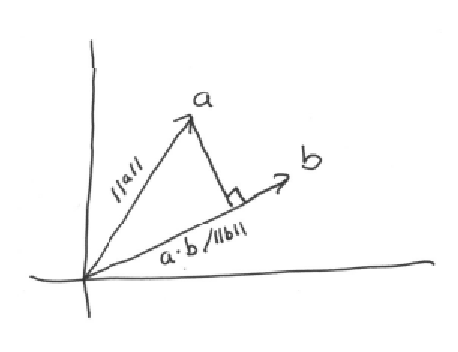
\includegraphics{projection.eps}

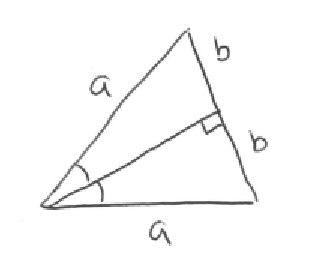
\includegraphics{isosoles_triangle.eps}

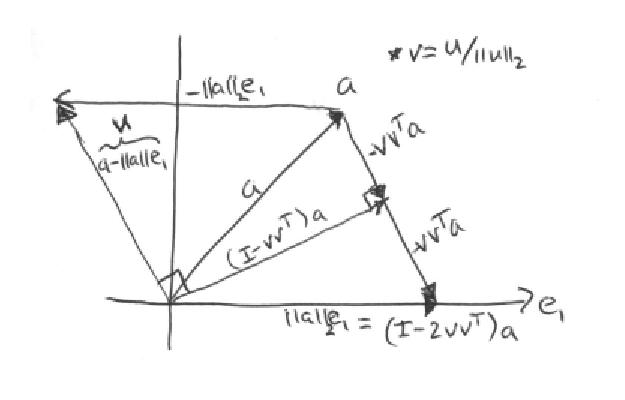
\includegraphics{householder.eps}


\section{Singular Value Decomposition}

The SVD is extremely stable and is in some sense the ultimate safe thing to do, if it is done right anyway.  We do not often do it as it is expensive (read slow) to calculate.  The danger in QR is in error buildup in solving, $R$, by back substitution.  It would be much nicer to have a diagonal matrix so errors couldn't buildup.  The SVD always exists and is a non-unique (i.e. there are many different SVD's for the same matrix) decomposition that is given by
\begin{eqnarray}
A &=& U\Sigma V^T
\end{eqnarray}
where $U$ and $V$ are unitary (generalization of orthogonal to complex numbers) matrices, and $\Sigma$ is  a diagonal matrix with the main diagonal ordered so $\sigma_1\geq\sigma_2\geq\cdots\geq\sigma_n\geq 0$.  Thus $\Sigma$ is not only diagonal, it is positive semidefinite (there could be zeros on the diagonal) and ordered.  We can even calculate individual singular values (the $\sigma_i$).  Some popular uses are
\begin{enumerate}
\item $\|A\|_2=\sigma_1$
\item $\|A^{-1}\|_2=\sigma_n^{-1}$
\item $cond(A)=\frac{\sigma_1}{\sigma_n}$
\item $\|A\|_{Frobenius}^2=\sum_{i=1}^n\sigma_i^2$
\item $A^{-1} = V\Sigma^{-1}U^T$, note $\Sigma^{-1}$ is easy to calculate because it is diagonal.
\end{enumerate} 
\chapter{Integration}\label{c-Integ}

The fundamental theorem of Calculus tells us that an integral of a
function can be expressed in terms of the anti-derivative of the
function.  Unfortunately, not all functions have anti-derivatives
that are expressible in known functions.  One of the most famous is
the Gaussian probability distribution, which is given by
\beqn
e^{-\left(\frac{x-\mu}{\sigma}\right)^{2}}.
\eeqn
The anti-derivative of this important and frequently occurring function
is unknown.  How do we handle it?  That is the subject of this chapter.

\section{Riemann}
We recall from Calculus that the integral is defined as
\beqn
\int_{a}^{b}{f(x)dx} =
\lim_{n\rightarrow\infty}\sum_{j=1}^{n}f(p_{j})(x_{j}-x_{j-1}).
\eeqn
Now assume that all $n$ of the $x_{j}$ are evenly spaced on $[a,b]$.  We
can then write
\beqn
h & = & \frac{b-a}{n} \\
  & = & x_{j}-x_{j-1}.
\eeqn
We can use this to get an expression for the Riemann Sum
\beqn
\int_{a}^{b}{f(x)dx}
 & = &
\lim_{n\rightarrow\infty}\sum_{j=1}^{n}f(p_{j})(x_{j}-x_{j-1}) \\
 & = &
\lim_{n\rightarrow\infty}\sum_{j=1}^{n}f(p_{j})h \\
 & = &
\lim_{n\rightarrow\infty}h\sum_{j=1}^{n}f(p_{j}).
\eeqn
To evaluate the integral numerically we are not able to take the
limit, so we get
\beqn
\int_{a}^{b}{f(x)dx}
 & \approx &
h\sum_{j=1}^{n}f(p_{j}).
\eeqn
The exact size of $n$ for the approximation to be good is a key aspect
of numerical integration.  Note also that I have not specified what
$p_{j}$ is, as this form allows you to do a left, right, mid-point,
maximum, or minimum.  The basic idea here is that we are approximating
the function by a constant on the interval.

\beqn
\int_{a}^{b}{f(x)dx}
 & \approx &
h\sum_{j=1}^{n}f(p_{j}).
\eeqn

Now we want to think about the error.  First we want to get an
expression for the integral in terms of an exact sum.  To do this we
use the fundamental theorem of calculus, add nothing, rearrange, and
use the mean value theorem.
\beqn
\int_{a}^{b}f(x)dx
& = &
F(b)-F(a) \\
& = &
F(x_{n})-F(x_{0}) \\
& = &
F(x_{n})+\sum_{i=1}^{n-1}(F(x_{i})-F(x_{i}))-F(x_{0}) \\
& = &
\sum_{i=1}^{n}(F(x_{i})-F(x_{i-1})) \\
& = &
\sum_{i=1}^{n}f(c_{i})(x_{i}-x_{i-1}) \\
& = &
\sum_{i=1}^{n}f(c_{i})h \\
& = &
h\sum_{i=1}^{n}f(c_{i})
\eeqn
This expression is exact so we can take it and subtract the
expression for the midpoint method.  We will assume the function has a
derivative and we will note that since we have picked the midpoint
that any other point in the interval is within half the width of the
interval of the midpoint.
\beqn
E
& = &
h\sum_{i=1}^{n}f(c_{i}) - h\sum_{i=1}^{n}f(p_{i}) \\
& = &
h\sum_{i=1}^{n}(f(c_{i}) - f(p_{i})) \\
& = &
h\sum_{i=1}^{n}f'(d_{i})(c_{i} - p_{i}) \\
& \leq &
h\sum_{i=1}^{n}f'(d_{i})\frac{h}{2} \\
& = &
\frac{h^{2}}{2}\sum_{i=1}^{n}f'(d_{i})
\eeqn
Recall that $h$ is inversely proportional to $n$, so we have that the
Error is inversely proportional to the square of $n$.

\section{Trapezoid}


\beqn
\int_{a}^{b}{f(x)dx}
 & \approx &
h\left(\frac{f(x_{0})+f(x_{n})}{2}+\sum_{j=1}^{n}f(x_{j})\right)
\eeqn


\section{Simpson}

\beqn
\int_{a}^{b}{f(x)dx}
 & \approx &
\frac{h}{3}\left(f(x_{0})+f(x_{n})+2\sum_{j=1}^{\frac{n}{2}-1}f(x_{2j})
+4\sum_{j=1}^{\frac{n}{2}}f(x_{2j-1})\right)
\eeqn

\section{Richardson}

Define the value of the integral to be $I$ and the numeric
approximation by some method at $n$ node points to be $I_{n}$.  We note that the error is of the form
\beqn
E
& = &
I-I_{n} \\
& = &
\frac{c}{n^{p}},
\eeqn
with $c$ a constant dependent on the function and $p$ a power dependent
on the method.  For midpoint and trapezoidal methods $p=2$, while for
Simpson's method $p=4$.  If we double the number of points then the
error would be
\beqn
E
& = &
I-I_{2n} \\
& = &
\frac{c}{2^{p}n^{p}} \\
& = &
\frac{1}{2^{p}}(I-I_{n}).
\eeqn
Solving for $I$ we find
\beqn
I-I_{2n}
& = &
\frac{1}{2^{p}}(I-I_{n}) \\
I-\frac{1}{2^{p}}I
& = &
I_{2n}\frac{1}{2^{p}}I_{n} \\
\frac{2^{p}-1}{2^{p}}I
& = &
I_{2n}-\frac{1}{2^{p}}I_{n} \\
I
& = &
\frac{2^{p}}{2^{p}-1}I_{2n}-\frac{1}{2^{p}-1}I_{n} \\
I
& = &
\frac{1}{2^{p}-1}\left(2^{p}I_{2n}-I_{n}\right).
\eeqn
This is Richardson's Extrapolation formula, and it will typically
give a big improvement to any of the methods.  We can use this
estimate of the error to calculate the error
\beqn
E
& = &
I-I_{2n} \\
& = &
\frac{2^{p}}{2^{p}-1}I_{2n}-\frac{1}{2^{p}-1}I_{n}-I_{n} \\
& = &
\frac{2^{p}-(2^{p}-1)}{2^{p}-1}I_{2n}-\frac{1}{2^{p}-1}I_{n} \\
& = &
\frac{1}{2^{p}-1}I_{2n}-\frac{1}{2^{p}-1}I_{n} \\
& = &
\frac{1}{2^{p}-1}(I_{2n}-I_{n}).
\eeqn
This is Richardson's error formula.  We note that we can get a
convergence rate by doing a little algebra on what we have already
found.
\beqn
I-I_{2n}
& = &
\frac{1}{2^{p}}(I-I_{n}) \\
\frac{I-I_{n}}{I-I_{2n}}
& = &
2^{p}
\eeqn
This is a nice equation but in general it is not calculable, as we
don't know $I$ and might not know p.  We can handle this by considering
the quantity
\beqn
\frac{I_{2n}-I_{n}}{I_{4n}-I_{2n}}
& = &
\frac{I_{2n}-I_{n}+I-I}{I_{4n}-I_{2n}+I-I} \\
& = &
\frac{(I-I_{n})-(I-I_{2n})}{(I-I_{2n})-(I-I_{4n})} \\
& = &
\frac{(I-I_{n})-\frac{1}{2^{p}}(I-I_{n})}{\frac{1}{2^{p}}(I-I_{n})-\frac{1}{4^{p}}(I-I_{n})} \\
& = &
\frac{1-\frac{1}{2^{p}}}{\frac{1}{2^{p}}(1-\frac{1}{2^{p}})} \\
& = &
\frac{1}{\frac{1}{2^{p}}} \\
& = &
2^{p}.
\eeqn
We thus have a simple way of calculating the convergence rate, and
thus a way to find $p$.

Homework: 7.1) 2(a), (b), (f) for midpoint, trapezoidal, and
simpson.  Compare with the error for trapezoidal (7.32) and
Richardson's extrapolation.

7.2) 8

\section{Gaussian Quadrature}

And now for something completely different\ldots

Last time we considered the standard way of thinking about integration, namely summing up a bunch of small areas.  The technique we will discuss today was introduced in 1814 by Gauss, hence the name.  We will now consider the integral
\beqn
I(f) = \int_{-1}^{1}f(t)dt.
\eeqn
Note that this is a perfectly general statement, as all we need to do to convert this to an integral of the form $\int_a^bf(x)dx$ is to find a linear mapping between the two intervals of integration:
\begin{eqnarray}
t&=& [-1,1]\\
x&=& [a,b]
\end{eqnarray}
We thus want to find a function $x=g(t)$ such that $a=g(-1)$, $b=g(1)$, and $g(\cdot)$ is linear.  We have two points which determine a line, so we can use the two-point formula for a line:
\begin{eqnarray}
m_g
&=& \frac{x_1-x_0}{t_1-t_0}\\
&=& \frac{b-a}{1--1}\\
&=& \frac{b-a}{2}\\
x
&=& x_1+m_g(t-t_1)\\
&=& b+\frac{b-a}{2}(t-1)\\
&=& \frac{1}{2}(2b+t(b-a)-(b-a))\\
&=& \frac{1}{2}(t(b-a)+b+a)\\
&=& \frac{t(b-a)+b+a}{2}
\end{eqnarray}
So, if we define $x=0.5(t(b-a)+b+a)$ and thus $dx=0.5(b-a)dx$ then we have\footnote{You will see some books define $t=(2x-a-b)/(b-a)$, and $dt=2dx/(b-a)$, which is the same formula but not as convenient for what we want.}
\beqn
\int_{a}^{b}{f(x)dx}
 & = &
\int_{g(-1)}^{g(1)}{f(x)g'(t)dt}\\
 & = &
\int_{-1}^{1}{f\left(\frac{(b-a)t+b+a}{2}\right)\left(\frac{b-a}{2}\right)dt}
\eeqn
We have that the integral is general, if not all that obvious as to why we chose this in the first place (it will become more apparent in a few moments).  We still need to show how to estimate the integral.  The basic idea is to approximate the integral by weighted evaluations of the function at a series of node points.  To get a good estimate we will require that our estimate at $n$ node points will be good for every polynomial up to order $2n-1$.  How?  Pick $w_{i}$ and $x_{i}$ such that
\beqn
I(f)=\sum_{i=1}^{n}w_{i}f(x_{i})
\eeqn
holds for all $f\in\{1,x,\ldots,x^{2n-1}\}$.  Let's do some examples.

\vspace{.1in}\noindent
\textbf{Example:}

Consider $n=1$.
\beqn
\int_{-1}^{1}dx
 & = &
w_{1}f(x_{1}) \\
2
 & = &
w_{1} \\
\int_{-1}^{1}xdx
 & = &
w_{1}x_{1} \\
0
 & = &
2x_{1} \\
0
 & = &
x_{1}
\eeqn

Also, consider $n=2$.
\beqn
\int_{-1}^{1}dx
 & = &
w_{1}f(x_{1})+w_{2}f(x_{2}) \\
2
 & = &
w_{1}+w_{2} \\
\int_{-1}^{1}xdx
 & = &
w_{1}f(x_{1})+w_{2}f(x_{2}) \\
0
 & = &
w_{1}x_{1}+w_{2}x_{2} \\
\int_{-1}^{1}x^{2}dx
 & = &
w_{1}f(x_{1})+w_{2}f(x_{2}) \\
\frac{2}{3}
 & = &
w_{1}x_{1}^{2}+w_{2}x_{2}^{2} \\
\int_{-1}^{1}x^{3}dx
 & = &
w_{1}f(x_{1})+w_{2}f(x_{2}) \\
0
 & = &
w_{1}x_{1}^{3}+w_{2}x_{2}^{3}
\eeqn
Solve these four equations for four unknowns and we find
\beqn
w_{1} & = & 1 \\
w_{2} & = & 1 \\
x_{1} & = & -\frac{1}{\sqrt{3}} \\
x_{1} & = & \frac{1}{\sqrt{3}}
%w_{2} & = & 2-w_{1} \\
%x_{2} & = & -\frac{w_{1}}{2-w_{1}}x_{1} \\
%w_{1} & = & -(2-w_{1})\left(\frac{-\frac{w_{1}}{2-w_{1}}x_{1}}{x_{1}}\right)^{2} \\
%x_{1} & = & \left(
%  \frac{2-w_{1}}{-(2-w_{1})\left(\frac{-\frac{w_{1}}{2-w_{1}}x_{1}}{x_{1}}\right)^{2}}
%  \right)^{\frac{1}{3}}
\eeqn
The node points turn out to be the roots of the Legendre
polynomials.  The Legendre polynomials are defined on $[-1,1]$ hence
our choice for the limits of integration.  You can find the Legendre
polynomials by the following properties.
\begin{itemize}
\item
$P_{n}$ is a polynomial of order $n$.
\item
They are orthogonal
\beqn
\int_{-1}^{1}P_{i}(x)P_{j}(x)dx=0
\eeqn
when $i\ne j$.
\item
The normalization is
\beqn
\int_{-1}^{1}P_{n}(x)^{2}dx=\frac{2}{2n+1}
\eeqn
\end{itemize}
The first several Legendre polynomials are
$\{1,x,x^{2}-\frac{1}{3},x^{3}-\frac{3}{5}x,x^{4}-\frac{6}{7}x^{2}+\frac{3}{35}\}$.

The constants can be found by
\beqn
w_{i}=\int_{-1}^{1}\prod_{j=1, j\ne i}^{n}\frac{x-x_{j}}{x_{i}-x_{j}}dx
\eeqn

In general we do not need to use this as the values are well tabulated, see for instance Table~\ref{t-gauss-quad}.


\begin{table}

  \centering
  \caption{Gauss-Legendre Abscissae and Weights to 8 Decimal Places}\label{t-gauss-quad}

\begin{tabular}{rr@{}llc}
n  & \multicolumn{2}{c}{Evaluation Points, $x_i$} & Weights, $w_i$ & Degree (2n-1) \\ \hline
1  & 0&.0                                         & 2.0            & 1 \\ \hline
2  & $\pm$&$\frac{1}{\sqrt{3}}$                   & 1.0            & 3 \\ \hline
3  & 0&.0                                         & 0.88888889     & 5 \\
   & $\pm$0&.77459667                             & 0.55555555     &   \\ \hline
4  & $\pm$0&.33998104                             & 0.65214515     & 7 \\
   & $\pm$0&.86113631                             & 0.34785485     &   \\ \hline
5  & 0&.0                                         & 0.56888889     & 9 \\
   & $\pm$0&.53846931                             & 0.47862867     &   \\
   & $\pm$0&.90617985                             & 0.23692689     &   \\ \hline
6  & $\pm$0&.23861918                             & 0.46791393     & 11 \\
   & $\pm$0&.66120939                             & 0.36076157     &   \\
   & $\pm$0&.93246951                             & 0.17132449     &   \\ \hline
7  & 0&.0                                         & 0.41795918     & 13 \\
   & $\pm$0&.40584515                             & 0.38183005     & \\
   & $\pm$0&.74153119                             & 0.27970539     & \\
   & $\pm$0&.94910791                             & 0.12948497     & \\ \hline
8  & $\pm$0&.18343464                             & 0.36268378     & 15 \\
   & $\pm$0&.52553241                             & 0.31370665     & \\
   & $\pm$0&.79666648                             & 0.22238103     & \\
   & $\pm$0&.96028986                             & 0.10122854     & \\ \hline
10 & $\pm$0&.14887434                             & 0.29552422     & 19 \\
   & $\pm$0&.43339539                             & 0.26926672     & \\
   & $\pm$0&.67940957                             & 0.21908636     & \\
   & $\pm$0&.86506337                             & 0.14945135     & \\
   & $\pm$0&.97390653                             & 0.06667134     & \\ \hline
\end{tabular}
\end{table}



Homework Redo 7.1) 2(a), (b), (f) for gaussian quadrature up to
$n=8$.  How does the convergence compare?


\chapter{Differentiation}

Numerical differentiation seems obvious.  In most introductions to calculus, the derivative is introduced as the limit of a series of secant lines.  Probably the most basic method of numerically taking the derivative is based off this formula.  It turns out that while it seems obvious, numerical derivatives are more difficult as we will see.

\section{Derivative Approximation}
Let's start at the basics, the two point method of obtaining the derivative is based off taking the derivative of the two point interpolation polynomial.
\beqn
f(x) & \approx &
   \frac{x_{1}-x}{h}f(x_{0})+\frac{x-x_{0}}{h}f(x_{1}) \\
f'(x) & \approx &
   \frac{-1}{h}f(x_{0})+\frac{1}{h}f(x_{1}) \\
 & = &
   \frac{f(x+h)-f(x)}{h}.
\eeqn
This is only exact when we take the limit as $h$ approaches zero.  We can see how the basic errors are dealt with by expanding the Taylor sequence.
\beqn
f(x+h)=f(x)+hf'(x)+\frac{h^{2}}{2}f''(c)
\eeqn
Using the Taylor series in the formula we obtain that the error in the
formula is
\beqn
E & = & f'(x)-\frac{f(x+h)-f(x)}{h} \\
& = & f'(x)-\frac{f(x)+hf'(x)+\frac{h^{2}}{2}f''(c)-f(x)}{h} \\
& = & f'(x)-\frac{hf'(x)+\frac{h^{2}}{2}f''(c)}{h} \\
& = & f'(x)-f'(x)+\frac{h}{2}f''(c) \\
& = & \frac{h}{2}f''(c).
\eeqn
Two other types of error occur.  First, there is subtractive difference errors.  We note that since $f(x)\approx f(x+h)$, when we
subtract them we will lose precision.  Second, there is error propagation.  Consider the fact that nothing we do in the real world is ever exact, so we actually measure and calculate a nearby solution:
\beqn
f(x) & = & \tilde{f}(x)+\epsilon_{1} \\
f(x+h) & = & \tilde{f}(x+h)+\epsilon_{2}.
\eeqn
Substituting this into our formula we find
\beqn
f'(x) & \approx &
   \frac{f(x+h)-f(x)}{h} \\
 & = &
   \frac{\tilde{f}(x+h)+\epsilon_{2}-\tilde{f}(x)+\epsilon_{1}}{h} \\
 & = &
   \frac{\tilde{f}(x+h)-\tilde{f}(x)}{h}+\frac{\epsilon_{2}-\epsilon_{1}}{h}.
\eeqn
The resulting error is
\beqn
E & = & f'(x)-\frac{f(x+h)-\epsilon_{2}-f(x)+\epsilon_{1}}{h} \\
& = & f'(x)-\frac{f(x)+hf'(x)+\frac{h^{2}}{2}f''(c)-\epsilon_{2}-f(x)+\epsilon_{1}}{h} \\
& = & f'(x)-\frac{hf'(x)+\frac{h^{2}}{2}f''(c)-\epsilon_{2}+\epsilon_{1}}{h} \\
& = & f'(x)-f'(x)+\frac{h}{2}f''(c)+\frac{\epsilon_{1}-\epsilon_{2}}{h} \\
& = & \frac{h}{2}f''(c)+\frac{\epsilon}{h}.
\eeqn
As long as the last term is non-zero, which it will be in general, if $h$ gets to small them the propagation errors dominate, see Figure~\ref{f-derivative_error}.  This is the real problem.  We did not have this problem with numerical integration because we were multiplying by $h$ rather than dividing by it.  The problem is more pronounced with higher order derivatives where you will be dividing by powers of $h$.  This problem motivates the use of integral equations rather than differential ones.  Unfortunately many integral equations are very ill-conditioned.  Anyway, the key idea is that there is a competition between several error types.


\begin{figure}
 \begin{center}
  \begin{lpic}{derivative_error(.5,.5)}
   \lbl[l]{2,75,90;Error}
   \lbl[b]{110,2,0;h}
  \end{lpic}
  \caption{Error in calculating the step size for different step sizes, $h$, for $f''(c)=2$ and $\epsilon=10^{-6}$.}\label{f-derivative_error}
 \end{center}
\end{figure}

\section{Tangent Line}

As of yet we have considered calculating the derivative from above.  Let us consider the derivative from below, and we will solve for it using the equation of a line and noting that the slope of the tangent line in the limit as $h=0$ is the derivative\footnote{We could have just used the same method we used in the last section, but what fun is that?}.
\beqn
y &=& mx+b \\
\eeqn
thus
\beqn
f(x) &=& mx+b \\
f(x-h) &=& m(x-h)+b.
\eeqn
Take the difference
\beqn
f(x)-f(x-h)
 &=& mx - m(x-h) \\
 &=& mh \\
m_{left} &=& \frac{f(x)-f(x-h)}{h}
\eeqn
This is the left approximation of the derivative and
\beqn
m_{right} &=& \frac{f(x+h)-f(x)}{h}
\eeqn
is the right approximation.  We get a better estimate by averaging them.
\beqn
m_{avg}
 &=&\frac{m_{left}+m_{right}}{2} \\
 &=&\frac{\frac{f(x)-f(x-h)}{h}+\frac{f(x+h)-f(x)}{h}}{2} \\
 &=&\frac{f(x)-f(x-h)+f(x+h)-f(x)}{2h} \\
 &=&\frac{f(x+h)-f(x-h)}{2h}
\eeqn
Interestingly the best thing we can do when we have three points is not to use the one we are trying to estimate the derivative of. The reason is, when we use the left approximation of the derivative, we are really estimating the derivative at $x-\frac{h}{2}$, and similarly for the right approximation.  By averaging we get an estimate of the derivative at $x$.

\section{Richardson Extrapolation}



\section{Higher Order Derivatives}

The second derivative is just the derivative of the first derivative.  Since the left and right approximations really give us the approximate derivative at $x\pm\frac{h}{2}$, we can use them, with their separation distance of $h$, to estimate the second derivative at $f(x)$.
\beqn
f''(x)
 &\approx& \frac{f'\left(x+\frac{h}{2}\right)-f'\left(x-\frac{h}{2}\right)}{h} \\
 &\approx& \frac{\frac{f(x+h)-f(x)}{h}-\frac{f(x)-f(x-h)}{h}}{h} \\
 &\approx& \frac{f(x+h)-2f(x)+f(x-h)}{h^2}
\eeqn
To solve for higher derivatives we will need more points: $f(x+2h)$, $f(x-2h)$, etc.  The further we go away the worse the approximation will be though, again showing that higher order derivatives become more inaccurate.

\subsection{Method of Undetermined Coefficients}

In addition to the point the derivative is to be evaluated at, we need one additional point per order of the derivative to be taken.  That is a first derivative takes 2 points, a second derivative takes 3 points, a third derivative takes 4, and so on.  Rather than memorize a bunch of formulas for higher powers, or even iterating the formula as above, we can use the method of undetermined coefficients, which can also be used for integration, interpolation, differential equations, etc.

Say we wanted to find the formula for the second derivative, which we know will require 3 points.
\begin{eqnarray*}
f''(x)=Af(x+h)+Bf(x)+Cf(x-h)
\end{eqnarray*}
We will use the Taylor Series to expand $f(x+h)$ and $f(x-h)$ around $x$.
\begin{eqnarray*}
f(x+h)=f(x)+hf'(x)+\frac{h^2}{2}f''(x)+hot \\
f(x-h)=f(x)-hf'(x)+\frac{h^2}{2}f''(x)+hot
\end{eqnarray*}
We now substitute this into the original expression.
\begin{eqnarray*}
f''(x)
&=&A\left(f(x)+hf'(x)+\frac{h^2}{2}f''(x)+hot\right)+Bf(x)+ \\
&&\qquad C\left(f(x)-hf'(x)+\frac{h^2}{2}f''(x)+hot\right) \\
&=& (A+B+C)f(x)+(A-C)hf'(x)+(A+C)\frac{h^2}{2}f''(x)+hot
\end{eqnarray*}
Equating like derivatives on the left and right we have

\begin{tabular}{ccc}
Derivative & Equation               & Implication \\\hline
$f(x)$     & $A+B+C=0$              & $B=-(A+C)$ \\
$f'(x)$    & $(A-C)h=0$             & $A=C$ \\
$f''(x)$   & $(A+C)\frac{h^2}{2}=1$ & $A=\frac{1}{h^2}$ \\
\end{tabular}

thus
\begin{eqnarray*}
f''(x)&=&\frac{1}{h^2}f(x+h)+\frac{-2}{h^2}f(x)+\frac{1}{h^2}f(x-h)\\
      &=&\frac{f(x+h)-2f(x)+f(x-h)}{h^2}.
\end{eqnarray*}
Note that we found the same formula a different way.

\chapter{Differential Equations}\label{c-DifEq}

Most practical problems will be described by a differential equation.
We will not in general know the form of the solution, but we usually
can find how they change with respect to each other.  From this basis
we would like to be able to find the actual solution.

\section{General Introduction}

Consider the general differential equation
\beq
\dot y(x)=f(x,y(x)). \label{DifEq-e1}
\eeq
Using basic calculus we see that the solution is given by
\beqn
y(x)=\int f(x,y(x))dx+c.
\eeqn
Often this is not very useful in solving equations however.  The way
to get practical solutions for this problem is covered in
differential equations, so I will just mention a few.

\subsection{Existence}
The problem~\ref{DifEq-e1} has a solution on an interval $x_{0}\leq x\leq
\min(b_{x},c)$ and $y_{0}\leq y\leq b_{y}$ if the function $f$ is continuous
on the interval for $c=\frac{\|y-y_{0}\|}{\max_{x,y}\left(\frac{\partial f(x,y)}
{\partial y}\right)}$.
\bfig
{\tt    \setlength{\unitlength}{0.92pt}
\begin{picture}(202,139)
\thinlines    \put(152,21){$c$}
              \put(155,104){\line(0,-1){73}}
              \put(40,31){\framebox(134,73){}}
              \put(40,31){\dashbox{5}(95,55){}}
              \put(135,85){\circle*{4}}
              \put(170,21){$b_x$}
              \put(28,101){$b_y$}
              \put(132,21){$x$}
              \put(33,82){$y$}
              \put(10,29){$y_0$}
              \put(38,12){$x_0$}
              \put(23,31){\vector(1,0){169}}
              \put(40,23){\vector(0,1){106}}
              \put(52,50){$f(x,y(x))$}
\end{picture}}
\efig{Existence requirements}{DifEq-f1}


\section{Euler's Method}

Euler was without a doubt one of the greatest mathematical minds to have ever lived.  He did work in almost every area you can imagine including numerical methods.  His method is simple and easy for people to use.  Unfortunately, as the old numerics folk theorem goes, ``that which is good for a person is bad for a computer and vise versa'' Euler's method is unstable numerically\footnote{The forward method actually, the backward method of Euler is stable though still far from a good method.}.  To introduce the method, say we knew a point, say $(x_0,y(x_0))$, we could denote our first point by the y-coordinate.
\beqn
y_{0} & = & y(x_0)
\eeqn
Now say we wanted to find the value of the function a short distance away, say at $x_0+h$.  It would be reasonable to do a first order taylor approximation.  Noting that $\dot y = f(x,y)$ allows us to write this in simple terms.
\beqn
y_{1} & = & y(x_{0}+h) \\
      & = & y_{0}+hf(x_{0},y_{0})
\eeqn
We could extend this process to find
\beqn
y_{n} & = & y(x_{0}+nh) \\
      & = & y_{n-1}+hf(x_{n-1},y_{n-1}) \\
      & = & y_{n-2}+hf(x_{n-2},y_{n-2})+hf(x_{n-2}+h,y_{n-2}+hf(x_{n-2},y_{n-2}))
\eeqn
Note that the third (last) term involves estimating based on an estimate.  It is here that the problem comes because the errors can build.  It is easier to show the problem by taking the \textit{Z}-Transform of the second line
\beqn
y_{n} & = & y_{n-1}+hf(x_{n-1},y_{n-1}) \\
Y & = & z^{-1}Y+hF(z^{-1}X,z^{-1}Y)
\eeqn
Assuming we are dealing with linear functions (a common assumption) we can pull the $z^{-1}$ out.
Error is given by
\beqn
Y(x)-y_{h}(x) & = & hD(x)+{\cal O}(h^{2}) \\
D'(x) & = & g(x)D(x)+\frac{1}{2}Y''(x), \qquad D(x_{o})=0 \\
g(x) & = & \left.\frac{\partial f(x,z)}{\partial z}\right|_{z=Y(x)}
\eeqn


\section{Runge-Kutta}

While Euler's method is nice and simple, it is far from the best.
Higher order Taylor methods can be derived but these require
evaluating multiple derivatives.  Even Richardson's extrapolation has
limits on its abilities.

Consider the Taylor series of $y$.
\beqn
y(x+h) & = & y(x)+hy'(x)+\frac{h^{2}}{2}y''(x)+\ldots \\
 & = & y(x)+hf(x,y)+\frac{h^{2}}{2}f'(x,y)+\ldots \\
 & = & y(x)+hf(x,y)+\frac{h^{2}}{2}\left(f_{x}(x,y)+f_{y}(x,y)f(x,y)\right)
        +\ldots \\
 & = & y(x)+hf(x,y)+\frac{h^{2}}{2}\left(f_{x}(x,y)+f_{y}(x,y)f(x,y)\right)
        +\ldots \\
 & = & y(x)+hf(x,y)+ah\left(\frac{h}{2a}f_{x}(x,y)+
           \frac{h}{2a}f(x,y)f_{y}(x,y)\right)
        +\ldots
\eeqn
Now we consider the Taylor series in two variables of $f(x,y)$.
\beqn
f(x+h,y+k) & = & \sum_{n=0}^{\infty}\frac{1}{n!}
 \left[h\frac{\partial}{\partial x}+k\frac{\partial}{\partial y}\right]^{n}f(x,y) \\
 & = & f(x,y)
 +\left[h\frac{\partial}{\partial x}+k\frac{\partial}{\partial y}\right]f(x,y)
 + \ldots \\
 & = & f(x,y)
 +hf_{x}(x,y)+kf_{y}(x,y)
 + \ldots
\eeqn
Rearranging we find
\beqn
f(x+h,y+k) -f(x,y)
  & = &
hf_{x}(x,y)+kf_{y}(x,y)
 + \ldots .
\eeqn
We use this in our Taylor series of $y$.
\beqn
y(x+h)
  & = & y(x)+hf(x,y)+ah\left(\frac{h}{2a}f_{x}(x,y)+\frac{h}{2a}f(x,y)f_{y}(x,y)\right)
        +\ldots \\
  & = & y(x)+hf(x,y)+h\left(af(x+\frac{h}{2a},y+\frac{h}{2a}f(x,y)) -af(x,y)\right)
        +\ldots \\
  & = & y(x)+h(1-a)f(x,y)+ahf(x+\frac{h}{2a},y+\frac{h}{2a}f(x,y))
        +\ldots \\
  & = & y(x)+h(1-a)f(x,y)+ahf(x+b,y+bf(x,y))
        +\ldots \\
& & \qquad b=\frac{h}{2a} \qquad 0\leq a \leq 1
\eeqn
We have defined this in order to take advantage of the many varieties
of second order R-K.  The most common are: Midpoint (a=1), Modified
Euler (a=1/2), and Heun's method (a=3/4).

You can also do R-K for higher orders.  The most common is fourth
order.  The algebra is tedious so I will just present the result.
\beqn
y(x+h) = y(x)+\frac{1}{6}\left(F_{1}+2F_{2}+2F_{3}+F_{4}\right)
\eeqn
with
\beqn
F_{1} & = & hf(x,y) \\
F_{2} & = & hf(x+\frac{h}{2},y+\frac{F_{1}}{2}) \\
F_{3} & = & hf(x+\frac{h}{2},y+\frac{F_{2}}{2}) \\
F_{4} & = & hf(x+h,y+F_{3})
\eeqn

\section{Fehlberg's Method}

We have seen that the local error (error in one step due mostly to
truncation) is one order of magnitude better than the global error,
in general.  Often we use Richardson's Error formula to find an
estimate of the local error ($T_{n}$) so we can adjust the step size
to keep things nice.  For instance Richardson's Error for Euler's
method gives us
\beqn
Y(x)-y_{h}(x) & \approx & hD(x) \\
Y(x)-y_{2h}(x) & \approx & 2hD(x) \\
Y(x)-y_{2h}(x) & \approx & 2(Y(x)-y_{h}(x)) \\
Y(x) & \approx & 2y_{h}(x)-y_{2h}(x) \\
Y(x)-y_{h}(x) & \approx & (2y_{h}(x)-y_{2h}(x))-y_{h}(x) \\
 & \approx & y_{h}(x)-y_{2h}(x).
\eeqn
This gives us a reasonable extrapolation formula, and estimate of the
error.  Another way to estimate the error would be to look at two
estimates from different order methods.  For instance you could do a
fourth and a fifth order R-K estimate at each step and use the
difference to bound the error.  If the error at any step became to
large then you would decrease the step size and try again.  This idea
is Fehlberg's method, and it is the basis of most modern ode solvers.
This is why Matlab has ode23 and ode45.

\section{Adams-Bashforth}

Up till now we have been looking at solving the differential equation
directly.  We could however just integrate both sides.
\beqn
y' & = & f(x,y) \\
\int_{x_{n}}^{x_{n+1}}y'dx & = & \int_{x_{n}}^{x_{n+1}}f(x,y)dx \\
y(x_{n+1})-y(x_{n}) & = & \int_{x_{n}}^{x_{n+1}}f(x,y)dx \\
y(x_{n+1}) & = & y(x_{n}) + \int_{x_{n}}^{x_{n+1}}f(x,y)dx
\eeqn
Our task is now reduced to trying to find the remaining integral,
which we can use the ideas we had from last chapter.  Adams-Bashforth
of order $m$ uses a polynomial approximation to $f(x,y)$ at the points
$x_{n}$, $x_{n-1}$, \ldots, $x_{n-m+1}$.  Consider the second order
Adams-Bashforth method.
\beqn
f(x,y(x)) & \approx &
  \frac{x_{n}-x}{h}f(x_{n-1})+\frac{x-x_{n-1}}{h}f(x_{n}) \\
\int_{x_{n}}^{x_{n+1}}f(x,y)dx & \approx &
  \int_{x_{n}}^{x_{n+1}}\left(
  \frac{x_{n}-x}{h}f(x_{n-1})+\frac{x-x_{n-1}}{h}f(x_{n})
  \right)dx \\
  & \approx &
  \left.
  \frac{x_{n}x-\frac{1}{2}x^{2}}{h}f(x_{n-1})+
  \frac{\frac{1}{2}x^{2}-x_{n-1}x}{h}f(x_{n})
  \right|_{x_{n}}^{x_{n+1}} \\
  & \approx &
  \frac{x_{n}h-\frac{x_{n+1}^{2}-x_{n}^{2}}{2}}{h}f(x_{n-1})+
  \frac{\frac{x_{n+1}^{2}-x_{n}^{2}}{2}-x_{n-1}h}{h}f(x_{n}) \\
  & \approx &
  \frac{x_{n}h-\frac{x_{n+1}^{2}-x_{n+1}x_{n}+x_{n+1}x_{n}-x_{n}^{2}}{2}}{h}f(x_{n-1}) \\
  & & \qquad +
  \frac{\frac{x_{n+1}^{2}-x_{n+1}x_{n}+x_{n+1}x_{n}-x_{n}^{2}}{2}-x_{n-1}h}{h}f(x_{n}) \\
  & \approx &
  \frac{x_{n}h-\frac{x_{n+1}h+x_{n}h}{2}}{h}f(x_{n-1})+
  \frac{\frac{x_{n+1}h+x_{n}h}{2}-x_{n-1}h}{h}f(x_{n}) \\
  & \approx &
  \frac{2x_{n}-(x_{n+1}+x_{n})}{2}f(x_{n-1})+
  \frac{x_{n+1}+x_{n}-2x_{n-1}}{2}f(x_{n}) \\
  & \approx &
  \frac{x_{n}-x_{n+1}}{2}f(x_{n-1})+
  \frac{x_{n+1}-x_{n-1}+x_{n}-x_{n-1}}{2}f(x_{n}) \\
  & \approx &
  \frac{-h}{2}f(x_{n-1})+\frac{2h+h}{2}f(x_{n}) \\
  & \approx &
  \frac{h}{2}(3f(x_{n})-f(x_{n-1}))
\eeqn
This is kind of ugly, so it would be nice to have a faster way of
handling things, especially as the dimensions increase.  Luckily there
is just such a technique.  The method of undetermined coefficients.  We start by assuming the general form we want, in this case,
\beqn
\int_{x_{n}}^{x_{n+1}}f(x,y)dx & \approx & af(x_n)+bf(x_{n-1}
\eeqn

We would like the approximation to work perfectly for constant and linear terms so:

Constant term, $f(x,y)=1$
\beqn
\int_{x_{n}}^{x_{n+1}}1dx & = & a\cdot 1+b\cdot 1 \\
h &=& a+b.
\eeqn

Linear term, $f(x,y)=x$
\beqn
\int_{x_{n}}^{x_{n+1}}xdx & = & a\cdot x_n+b\cdot x_{n-1} \\
\frac{x_{n+1}^2-x_n^2}{2} &=& a\cdot x_n-a\cdot x_{n-1}+a\cdot x_{n-1}+b\cdot x_{n-1} \\
\frac{x_{n+1}^2-x_nx_{n+1}+x_nx_{n+1}-x_n^2}{2} &=& a\cdot(x_n-x_{n-1})+(a+b)\cdot x_{n-1}.
\eeqn
Now noting that $a+b=h$
\beqn
\frac{x_{n+1}(x_{n+1}-x_n)+x_n(x_{n+1}-x_n)}{2} &=& a\cdot(h)+(h)\cdot x_{n-1} \\
\frac{x_{n+1}h+x_nh}{2} &=& a\cdot h+h\cdot x_{n-1} \\
\frac{x_{n+1}+x_n-2x_{n-1}}{2} &=& a \\
\frac{x_{n+1}-x_{n-1}+x_n-x_{n-1}}{2} &=& a \\
\frac{2h+h}{2} &=& a \\
\frac{3h}{2} &=& a.
\eeqn

Thus since $a+b=h$,
\beqn
b=\frac{-h}{2}
\eeqn
which is what we found before.

\section{Adams-Moulton}

Adams-Bashforth considered that we knew only up to $f(x,y)$ only at points up to $x_n$.  What if we assume we can use $x_n$ or a near approximation?  Let us again consider just the simple case of linear approximations to function, though we could use any order of polynomial we liked (if we want to do the work).
\beqn
f(x,y(x)) & \approx &
  \frac{x-x_{n}}{h}f(x_{n+1})+\frac{x_{n+1}-x}{h}f(x_{n})
\eeqn
Using this we can solve the integral.
\beqn
\int_{x_{n}}^{x_{n+1}}f(x,y)dx & \approx &
  \int_{x_{n}}^{x_{n+1}}\left(
  \frac{x-x_{n}}{h}f(x_{n+1})+\frac{x_{n+1}-x}{h}f(x_{n})
  \right)dx \\
  & \approx &
  \left.
  \frac{\frac{1}{2}x^{2}}{h}f(x_{n+1}-x_{n}x)+
  \frac{x_{n+1}x-\frac{1}{2}x^{2}}{h}f(x_{n})
  \right|_{x_{n}}^{x_{n+1}} \\
  & \approx &
  \frac{\frac{x_{n+1}^{2}-x_n^{2}}{2}-x_nx_{n+1}+x_n^2}{h}f(x_{n+1})+
  \frac{x_{n+1}^2-x_{n+1}x_n-\frac{x_{n+1}^{2}-x_n^{2}}{2}}{h}f(x_{n}) \\
  & \approx &
  \frac{x_{n+1}^{2}-x_n^{2}-2x_nx_{n+1}+2x_n^2}{2h}f(x_{n+1})+
  \frac{2x_{n+1}^2-2x_{n+1}x_n-x_{n+1}^{2}+x_n^{2}}{2h}f(x_{n}) \\
  & \approx &
  \frac{x_{n+1}^{2}-2x_nx_{n+1}+x_n^2}{2h}f(x_{n+1})+
  \frac{x_{n+1}^2-2x_{n+1}x_n-+x_n^{2}}{2h}f(x_{n}) \\
  & \approx &
  \frac{(x_{n+1}-x_n)^2}{2h}f(x_{n+1})+
  \frac{(x_{n+1}-x_n)^2}{2h}f(x_{n}) \\
  & \approx &
  \frac{h^2}{2h}f(x_{n+1})+\frac{h^2}{2h}f(x_{n}) \\
  & \approx &
  \frac{h}{2}(f(x_{n+1})+f(x_{n}))
\eeqn


\section{Stability \& Stiff Equations}
A good start for looking at stiff equations is to examine the
stability of our methods.  Consider Forward Euler for
\beqn
y'=-200y, \qquad y(1)=e^{-200}.
\eeqn
The solution can easily be seen to be $e^{-200x}$.  Forward Euler
gives us
\beqn
y_{i+1} & = & y_{i}-200*h*y_{i} \\
 & = & y_{i}(1-200*h).
\eeqn
We note that this is stable if $\| 1-200*h \|<1$.  Since $h>0$ we
must have $h<0.01$.  This is a smooth, monotonically decreasing
function that is less than $2\time10^{-87}$ and greater than zero.
Despite the smoothness and flatness, we have to take very small
steps.  To see this look at Figure~\ref{stabfig}.
\begin{figure}[h]
\begin{center}
\leavevmode
\hbox{
\epsfxsize=4in
\epsffile{stab.eps}}
\end{center}
\caption{Instability in Euler's Method}
\label{stabfig}
\end{figure}
Note that Backward Euler does not have the same problem.  It is
defined by
\beqn
y_{i+1} & = & y_{i}-200*h*y_{i+1} \\
 & = & y_{i}\frac{1}{1+200*h},
\eeqn
which is stable for all $h>0$. Stability is not the same thing as
stiffness, but they are related.  Stiffness is due to multiple scales
of the terms, for instance $e^{-x}$, $e^{-200x}$.  Consider the
following equation
\beqn
0=\ddot{y}+1001\dot{y}+1000y, \qquad y(0)=1, \qquad \dot{y}(0)=-1.
\eeqn
The solution can easily be seen to be $e^{-t}$, which is nice in any
definition.  We solve the equation using a 4th order R-K method.  The
results are in Figure~\ref{stifffig}.
\begin{figure}[h]
\begin{center}
\leavevmode
\hbox{
\epsfxsize=6in
\epsffile{stiff.eps}}
\end{center}
\caption{Stiff Equation}
\label{stifffig}
\end{figure}

What is going on?  We need to look at the eigenvalues.

Define the intermediate variable $z=\dot y$, and the equation becomes
\beqn
0&=&\dot z +1001z+1000y \\
\dot z&=&-1001z-1000y.
\eeqn
Putting this in matrix form
\beqn
\dot{\bmat y\\z \emat} &=&\bmat 0 & 1 \\ -1000 & -1001 \emat \bmat y\\z\emat
\eeqn
The eigenvalues are (-1,-1000).  Since the eigenvalues differ by three orders of magnitude we can expect stiffness, which is what Figure~\ref{stifffig} shows.


\chapter{Modeling and Simulation}\label{c-ModSim}

Some systems cannot be practically tested.  Consider the spread of a highly infectious disease, or the destruction due to a nuclear war.  We can look at smaller examples of these, but the full blown case would be bad to run.  What we would like to do is to take our mathematical knowledge and create a system of equations which will have the same behavior.  We can then test the real system by seeing how the modeled system behaves.  This action of making a a mathematical model be similar to the real system is simulation (same root as similar).  Often these systems are expressed as either differential or difference equations.  They can thus be solved by our differential equation solvers directly, or transformed (Laplace, Fourier, Z, etc.) so they can be solved by zero-finding.

Lets look at how we can set some of these up, and then give some examples.

\subsection{Electric Circuit}
Kirkoff's law tells us that the sum of the voltage drops around a loop must be zero.  We can use this to figure out how to set up some models.  To do so we need to note how each element operates.  On the attached sheets I have included some copies of physical elements and how they relate.  If we consider our basic variable as charge then current is just the time derivative of charge and we can see the elements are just:
\beqn
V_{inductor} & = & L\ddot{q} \\
V_{resistor} & = & R\dot{q} \\
V_{capacitor} & = & \frac{1}{C}q
\eeqn
We can then write an equation for each loop and plot the first derivative of each of the loop charges (thus loop current).

\subsubsection{Low Pass Filter}

The sums of the voltage drops around the loop is
\begin{eqnarray}
V_{in} - R\dot q -\frac{1}{C}q &=& 0\label{eq-diffeqmodel-lowpassfilter}
\end{eqnarray}
The output voltage is the voltage across the capacitor, so
\begin{eqnarray}
V_{out} &=&\frac{1}{C}q
\end{eqnarray}
We thus need to find $q$, and we know (rearranging eq~\ref{eq-diffeqmodel-lowpassfilter})
\begin{eqnarray}
\dot q &=& \frac{V_{in}}{R} -\frac{1}{RC}q
\end{eqnarray}
This equation becomes code~\ref{code:lowpass}.
\SciLab{Code for the differential equation describing a low pass filter.}{code:lowpass}{scilab/lowpass.sci}
When called by
\SciLab{Code to simulate a low pass filter using RK 2nd order.}{code:lowpassfilter}{scilab/lowpassfilter.sce}

\begin{figure}
\begin{center}
\caption{Input and output voltages of the low pass filter.}
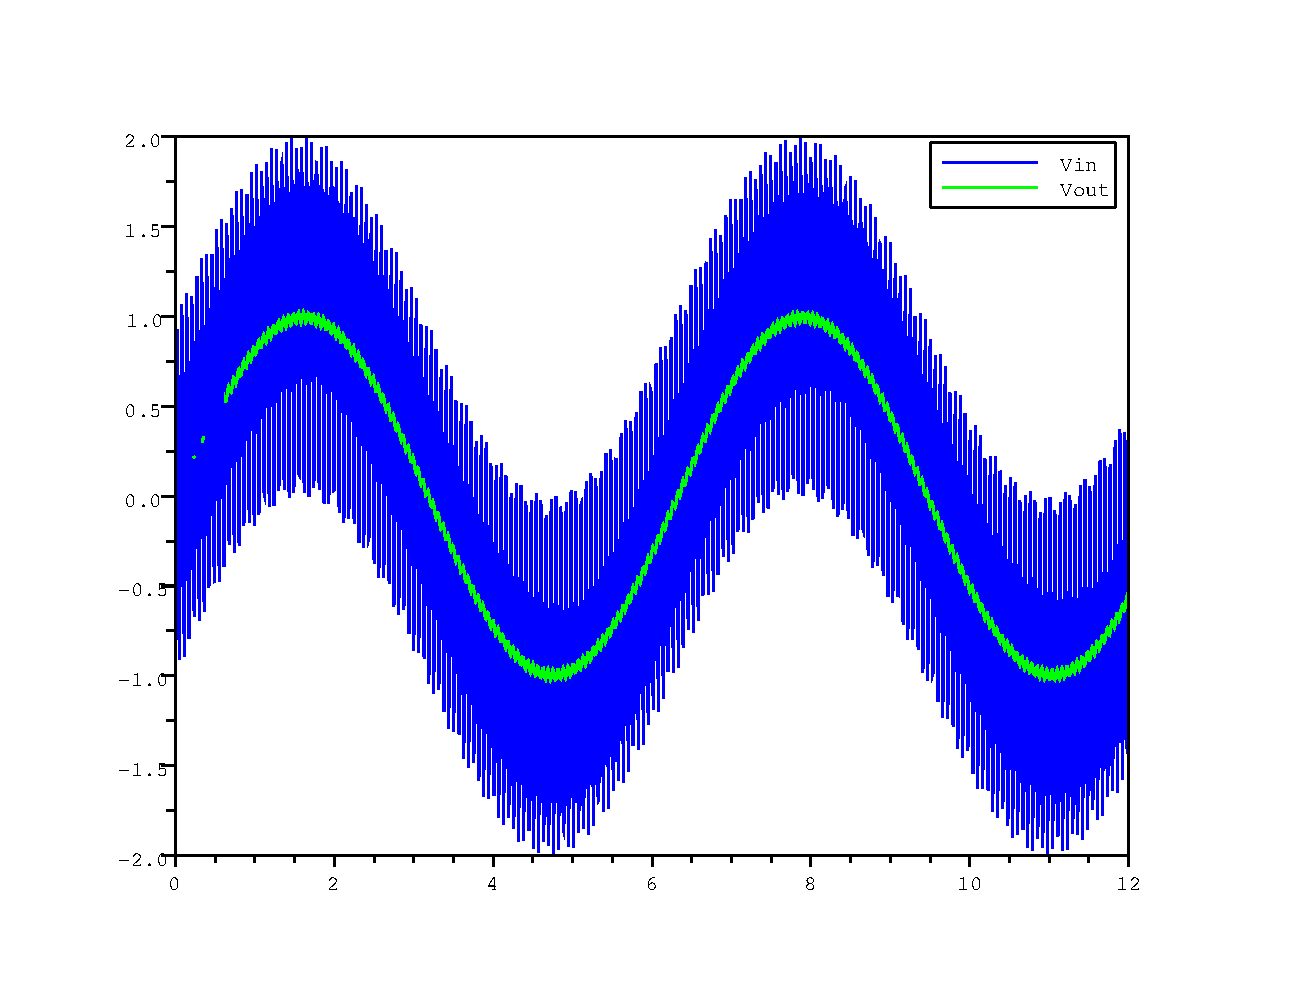
\includegraphics[width=.8\textwidth]{lowpass}
\end{center}
\end{figure}

\subsection{System of Masses}
Consider a system of masses connected by springs and dampers.  We can note that the if we choose our variable to be position then we have:
\beqn
F_{spring} & = & -kx \\
F_{damper} & = & -c\dot{x} \\
F_{mass} & = & m\ddot{x}
\eeqn

\subsection{Linearized Pendulum}
\beqn
\dot{\left[\begin{matrix}x_{1}\cr
                   x_{2}\end{matrix}\right]}
=
\left[\begin{matrix}0 & 1\cr
              -\sqrt{\frac{g}{l}}  & -c\end{matrix}\right]
\left[\begin{matrix}x_{1}\cr
              x_{2}\end{matrix}\right]
\eeqn


\subsection{Fox and Rabbits}

Consider the problem where there is a predator and its prey in the area.  If there are too many predators they might eat off all the prey and starve themselves.  If there are too much of the prey the predators will increase in number because of the plentiful food.  How do we model this?

We want several things in our model. First, predators should naturally starve, only the presence of prey offsets this.  Prey should naturally breed, and predators offset this.  The offset to both should be a scaled proportion of the contacts.  Contact should be rare when either population is low and more frequent with a reasonable number of both.  These considerations lead to the model that contacts occur at a rate proportional to the product of predators and prey.  These rules are combined in the model below.

\beqn
\dot{\bmat x_{1}\cr
           x_{2}\emat}
&=&
\bmat -m_{1} & 0\cr
       0     & m_{2}\emat
\bmat x_{1}\cr
      x_{2}\emat+
\bmat  b_{1}x_{1}x_{2}\cr
      -b_{2}x_{1}x_{2}\emat \\
&=&
\bmat b_{1}x_{2}-m_{1} & 0\cr
      0                & m_{2}-b_{2}x_{1}\emat
\bmat x_{1}\cr
      x_{2}\emat
\eeqn

To keep the population constant in each we need $b_{1}x_{2}-m_{1}=0$ and $m_{2}-b_{2}x_{1}=0$, thus
\beqn
x(1)&=&\frac{m_2}{b_2} \\
x(2)&=&\frac{m_1}{b_1}
\eeqn

We can implement the basic predator prey rate calculations by the Scilab function
\begin{verbatim}
function [xdot]=predator_prey_rate(starve,birth,eat,eaten,predator,prey)
    xdot=zeros(2,1);
    xdot(1)=(eat*prey-starve)*predator;
    xdot(2)=(birth-eaten*predator)*prey;
endfunction
\end{verbatim}
To specialize this to our foxes and rabbits we could write the Scilab function
\begin{verbatim}
function [xdot]=fox_rabbit(t,x)
    starve=5;
    birth=10;
    eat=.01;
    eaten=.5;
    predator=x(1);
    prey=x(2);
    getf('predator_prey_rate.sce');
    xdot=predator_prey_rate(starve,birth,eat,eaten,predator,prey);
endfunction
\end{verbatim}
Now we need to solve it, so we will use the function ode.  The following code will set everything up for us and call ode.
\begin{verbatim}
getf('fox_rabbit.sce');
x=ode([22;500],0,[0:.01:10],fox_rabbit);

//set("figure_style","new") //create a figure
subplot(211)
   plot2d([0:.01:10],x')
   xtitle('Fox and Rabbit History','Years','Population');
subplot(212)
   plot2d(x(1,:),x(2,:))
   xtitle('Fox and Rabbit Interaction','Foxes','Rabbits');
\end{verbatim}
When we run it we get the following graphic.
\begin{figure}[h]
\begin{center}
\leavevmode
\hbox{
\epsfxsize=6in
\epsffile{foxesNrabbits2.eps}}
\end{center}
\caption{Foxes and Rabbits}
\label{f-foxrabbit}
\end{figure}


\subsection{Arms race}
\beqn
\dot{\left[\begin{matrix}x_{1}\cr
                   x_{2}\end{matrix}\right]}
=
\left[\begin{matrix}-m_{1} & a_{1}\cr
              a_{2}  & -m_{2}\end{matrix}\right]
\left[\begin{matrix}x_{1}\cr
              x_{2}\end{matrix}\right] +
\left[\begin{matrix}b_{1}x_{2}^{2}\cr
              b_{2}x_{1}^{2}\end{matrix}\right]
\eeqn

\chapter{Partial Differential Equations}

\section{Basics}

Consider the equation
\begin{eqnarray}
f(x,t) &=& e^{kt}\sin({k\pi x}).
\end{eqnarray}
Assume for the moment that $x$ is constant and take the derivative with respect to $t$.  We will use the notation of $\partial$ to denote a derivative with respect to only one variable, also known as a partial derivative.
\begin{eqnarray}
\frac{\partial}{\partial t}f(x,t)
 &=& ke^{kt}\sin({k\pi x}) \\
 &=& f_t(x,t)
\end{eqnarray}


\section{Wave in a String}

Assume we have stretched a string to length $L$ and fixed it at both ends.  We want to find the function, $u(x,t)$, which describes the displacement of the string at any point.  Now we will consider the basic one-dimensional wave equation,
\begin{eqnarray}
\frac{1}{c^2}u_{tt} &=& u_{xx}. \label{eq-wave-string}
\end{eqnarray}
We will try one of the basic techniques, called separation of variables.  Basically we posit a solution of the form
\begin{eqnarray}
u(x,t) &=& f(x)g(t).
\end{eqnarray}
Substitute this back into Eq.~\ref{eq-wave-string}, we obtain
\begin{eqnarray}
\frac{1}{c^2}f(x)g''(t) &=& f''(x)g(t) \\
\frac{-k^2}{c^2}f(x)g''(t) &=& -k^2f''(x)g(t),
\end{eqnarray}
with $k$ a constant, which does not effect the equality but does provide a useful term when we solve later.  To maintain the independence between the $x$ and $t$ terms called for in the separation of variables technique it must be that the $x$ terms on the left and right must be equal (similar for the $t$ terms).  Thus we have that
\begin{eqnarray}
-k^2f(x) &=& f''(x) \\
\frac{1}{c^2}g''(t) &=& -k^2g(t),
\end{eqnarray}
and thus
\begin{eqnarray}
f''(x)+k^2f(x) &=& 0 \label{eq-wave-fx}\\
g''(t) +c^2k^2g(t) &=& 0 \label{eq-wave-gt},
\end{eqnarray}
where we have kept the constant $k$ with the terms that have no derivative\footnote{This is a result of experience.  Essentially doing this provides a constant to be solved for in each, and also couples the equations.}.  These are now ODE's, and we can now use the boundary conditions to solve them.  We will use the fact that differential equations can be expanded in terms of exponentials, since the derivative of an exponential is an exponential.  Second order differentials without a first order term are trigonometric functions\footnote{This can be understood from the fact that the second derivative of sine or cosine is the negative of itself.  It can also be seen from the fact that $e^{-j\phi}=\cos\phi+j\sin\phi$, where $j=\sqrt{-1}$.}.

First note that the boundary condition on the ends is that they are fixed.  This means that
\begin{eqnarray}
f(0)&=&0\\
f(L)&=&0.
\end{eqnarray}
This implies that 
\begin{eqnarray}
f(x)&=&\sum_{m=1}^{\infty}a_m\sin\left(\frac{2m\pi x}{L}\right).\label{eq-wave-xtrig}
\end{eqnarray}
We can now substitute Eq~\ref{eq-wave-xtrig} into Eq~\ref{eq-wave-fx}.
\begin{eqnarray}
-\sum_{m=1}^{\infty}a_m\left(\frac{2m\pi}{L}\right)^2\sin\left(\frac{2m\pi x}{L}\right)+k^2\sum_{m=1}^{\infty}a_m\sin\left(\frac{2m\pi x}{L}\right)&=&0\\
\sum_{m=1}^{\infty}a_m\left(k^2-\left(\frac{2m\pi}{L}\right)^2\right)\sin\left(\frac{2m\pi x}{L}\right)&=&0\\
k&=&\frac{2m\pi}{L}
\end{eqnarray}



\subsection{Partial Discretization}

Another way to solve this is to approximate the spatial derivative (discretizing in space), while leaving the time derivative alone.  The result is an ODE that approximates the PDE.  Say we use the basic higher order derivative formula we developed in the chapter on derivatives, with a step size of $\Delta$, then
\beqn
\frac{1}{c^2}u_{tt} &=& u_{xx} \\
\frac{1}{c^2}u_{tt}(t,x_i) &=& \frac{u(t,x_{i+1})-2u(t,x_i)+u(t,x_{i-1})}{\Delta^2} \\
u''(t,x_i) &=& \frac{-2c^2}{\Delta^2}u(t,x_i) + \frac{c^2}{\Delta^2}\left(u(t,x_{i+1})+u(t,x_{i-1})\right).
\eeqn
The last line just underscores that $u$ is now only a continuous function of $t$ described by a simple ODE.  In essence we have made a whole bunch of interconnected wave functions, one at each $x_i$.  This can be solved by any of the methods in the chapter on differential equations. 


\part{Numerical Linear Algebra}

\chapter{Vector Spaces}

In this chapter I will give the background material needed to understand numerical linear algebra.

\section{Basis}\label{s-basis}
To understand what a basis is, you first need to understand orthogonality and independence.  I will give you both some formal definitions, but more importantly I will try to make them understandable.  Let's start with independence.

\subsection{Independence}
Say we have a group of vectors $v_1, \ldots, v_n$.  We might want to know if there are any of them that are unnecessary, that is could we make it from a combination of the others.  If no vectors are unnecessary, we say the vectors are independent.  Formally, we write $v_1, \ldots, v_n$ are independent iff,
\begin{equation}
\sum_{i=1}^n\alpha_iv_i=0 \implies \alpha_i=0 \forall i\in\left\{1, \ldots, n\right\}
\end{equation}
In English, this reads the vectors $v_1, \ldots, v_n$ are independent if and only if the sum of each vectors $v_i$ times a scalar $\alpha_i$ for $i=1$ to $n$ is zero implies that all the $\alpha_i$ are zero.  In simple terms there is no non-zero weighted combinations of the vectors that sums to zero, as this would mean we could write one vector in terms of the others by some algebra.  The concept is not that tough but it can get a little messy when calculating, particularly when you are first introduced to the idea.

Let's do an example,
\begin{example}
Are the following two dimensional vectors independent?
\begin{eqnarray}
v_1=\left[\begin{matrix}1\\0\end{matrix}\right], v_2=\left[\begin{matrix}1\\1\end{matrix}\right]
\end{eqnarray}
\Solution
Let's write out the linear combination used in the definition.
\begin{eqnarray}
\sum_{i=1}^n\alpha_iv_i&=&0\\
\alpha_1v_1+\alpha_2v_2=0
\end{eqnarray}
Now this implies two equations (one for each row of the vectors).
\begin{eqnarray}
\alpha_1+\alpha_2 &=& 0\label{ex-linear_independence_simple2d_a}\\
\alpha_2&=&0\label{ex-linear_independence_simple2d_b}
\end{eqnarray}
Equation~\ref{ex-linear_independence_simple2d_b} tells us that the second scalar weight, $\alpha_2$ must be zero, which combined with Equation~\ref{ex-linear_independence_simple2d_a} requires the first scalar weight, $\alpha_1$, to be zero.  Thus by the definition, we have that the vectors are independent.
\end{example}

Now let's consider how many linearly independent vectors there could be, for a vector space of size $n$, where the size of the space is the number of elements in the vector.  It turns out that we can have $n$ of them.  The easiest way to see this is to consider the vectors $e_i$, which are vectors with all zero entries except one, which is a 1 in the i$^{th}$ position.  Trivially these vectors are independent (the summation in the definition results in $n$ equations of $\alpha_i=0$), so there are at least n independent vectors that span the space.  Could we add one more and still have linear independence?  Well consider the following.
\begin{enumerate}
\item The new vector cannot be all zeros or the $\alpha$ associated with it, say $\alpha_{n+1}$, could be any number to satisfy the sum since the vector would be zero and $\alpha_{n+1}\cdot 0=0$.
\item The new vector, say $d$, must have more than one non-zero term, since if it only had one it would trivially be one of the $e_i$ times a scalar equal to it's i$^{th}$ component ($d_i$) and thus as a duplicate, you would just have to pick $\alpha_i=-\alpha_{n+1}d_i$ to satisfy the summation without have all $\alpha_i$ zero.
\item An induction argument can be easily constructed now, by noting that adding one more non-zero component to $d$, say in position $j$, just requires setting $\alpha_j=-\alpha_{n+1}d_j$, to satisfy the sum without having all $\alpha_i$ zero.
\end{enumerate}
Thus we can see that we cannot add another vector, and thus the maximum number of independent vectors is $n$.  This is not yet a formal proof, many books include one, my purpose is to have you understand the what and the why parts.  You are encouraged to study the formal proofs on your own.

One other term often used is a basis.  A basis is a group of independent vectors that span a space (span means to cover all of it, and thus there will be a vector for each dimension in the space).

\subsection{Orthogonality}
To discuss orthogonality, I need to have an inner product.  Mathematicians use the notation $<a,b>$ to denote the inner product of $a$ and $b$.  Physicists use $a\cdot b$ for the same thing, unless they are doing quantum, in which case they use $<a|b>$.  In linear algebra you will often see this as $a^Tb$ if the vectors are real, or $a^Hb$ if they are complex\footnote{Some old texts use $a^*b$ for complex vectors, but it means the same thing as $a^Hb$.  In any case it denotes transposing and taking the complex conjugate (this is the star notation), which is called the hermitian transpose (this is the H notation).}.  I mention all these different ways of writing it as you might run into them in different contexts and you should realize they are the same.  For linear algebra we just mean to multiply the corresponding elements of the matrix and sum them up.
\begin{eqnarray}
a^Tb &=& \sum_{i=1}^na_ib_i
\end{eqnarray}
Just for your information this can be extended to infinite dimensional spaces like  the space of continuous functions on the interval from 0 to 1 by converting the sum into an integral, thus yielding
\begin{eqnarray}
<a(x),b(x)> &=& \int_{0}^1a(x)b(x)dx
\end{eqnarray}
Getting back to our main point, which is given an inner product, we can find the angle between the vectors.  How you ask?  Well, it turns out that
\begin{eqnarray}
a^Tb &=& \|a\|_2\|b\|_2\cos\theta
\end{eqnarray}
Where $\|\cdot\|_2$ is the 2 norm (described in Section~\ref{s-vect-norm}) and $\theta$ is the angle between the vectors $a$ and $b$.  The net result is that we can measure the angle between to vectors using the inner product.  If the inner product is zero and the vectors aren't zero, that means that the cosine must be.  For the cosine to be zero, the angle must be $\frac{\pi}{2}$ radians (or $90^\circ$ if you prefer).  Things that are $\frac{\pi}{2}$ radians apart are called orthogonal, so if the inner product of two vectors is zero, then the are orthogonal.  A lot of our algorithms force use the inner product to measure the angle between two vectors, and then using this measure construct an vector from one of them, that is orthogonal to the other.  If you understand this is what they are doing it makes the code much easier to read.

A neat side result is that if a group of vectors are mutually orthogonal, then they are also independent.


\section{Vector Norms}\label{s-vect-norm}

\subsection{Schatten P-Norms}

The basic definition for some whole number, $p$, and vector, $x\in\mathbb{R}^n$, is
\begin{eqnarray}
\| x \|_p &=& \sqrt[p]{\sum_{i=1}^{n}|x_i|^p},
\end{eqnarray}

Three special cases are most important, $p=1$, $p=2$, and $p=\lim_{k\rightarrow\infty}k$.

\subsubsection{Manhattan Norm}
Also called the one norm and the taxicab norm, this norm is the case when $p=1$.
\begin{eqnarray}
\| x \|_1 &=& \sqrt[1]{\sum_{i=1}^{n}|x_i|^1}\\
&=& \sum_{i=1}^{n}|x_i|
\end{eqnarray}
It is readily observed that this is simply the sum of the absolute values of the elements of the vector.

\subsubsection{Euclidian Norm}
Also known as the two norm, this norm is what most people think of as distance.
\begin{eqnarray}
\| x \|_2 &=& \sqrt[2]{\sum_{i=1}^{n}|x_i|^2} \\
&=& \sqrt{x^Tx}
\end{eqnarray}

\subsubsection{Infinity Norm}
This norm has a simple form that is not obvious at first
\begin{eqnarray}
\| x \|_{\infty} &=& \lim_{p\rightarrow\infty}\sqrt[p]{\sum_{i=1}^{n}|x_i|^p}
\end{eqnarray}

\subsection{Equivalence}
All the norms on a vector space are equivalent, by which we mean they for any two norms $\|\cdot\|_a$ and $\|\cdot\|_b$, and two scalars $\alpha$ and $\beta$, which depend only on the types of norms and dimension of the space, we have $\alpha\|x\|_a\leq\|x\|_b\leq\beta\|x\|_a \forall x$ in the vector space.  For instance, we have for the three most common Schatten P-Norms

\noindent
\begin{tabular}{lccc}
                 & $\|x\|_1$                                         & $\|x\|_2$                                              & $\|x\|_\infty$                                    \\
$\|x\|_1$        & $\|x\|_1\leq\|x\|_1\leq\|x\|_1$                   & $\|x\|_2\leq\|x\|_1\leq\sqrt{n}\|x\|_2$                & $\|x\|_\infty\leq\|x\|_1\leq n\|x\|_\infty$       \\
$\|x\|_2$        & $\frac{1}{\sqrt{n}}\|x\|_1\leq\|x\|_2\leq\|x\|_1$ & $\|x\|_2\leq\|x\|_2\leq\|x\|_2$                        & $\|x\|_\infty\leq\|x\|_2\leq\sqrt{n}\|x\|_\infty$ \\
$\|x\|_\infty$   & $\frac{1}{n}\|x\|_1\leq\|x\|_\infty\leq\|x\|_1$    & $\frac{1}{\sqrt{n}}\|x\|_2\leq\|x\|_\infty\leq\|x\|_2$ & $\|x\|_\infty\leq\|x\|_\infty\leq\|x\|_\infty$    \\
\end{tabular}

Note that the bounds are tight, which means that there are vectors x for which the equalities hold, though obviously not at the same time.  For instance if $x$ was an n-vector of ones, then $\|x\|_1=n\|x\|_\infty$.  Another example would be if $x=e_i$ were $e_i$ is a vector of zeros, with a single 1 in the i$^{th}$ position, in which case all the p-norms yield the same value (1).  One final note, the diagonal entries just say that the $i$ norm is equal to itself, while remaining the structure of the rest of the entries.

\chapter{Matrix Preliminaries}\label{c-matrix}

Matrices are an essential tool in control systems design.  First lets discuss some basic terms.
\begin{description}
    \item[$\RE$] The real numbers.
    \item[$\REn$] The vectors composed of n-tuples of real numbers.
    \item[$\REmn$] The matrices composed of m rows and n columns of real numbers.
\end{description}

\section{Addition and Subtraction}

In order to add or subtract matrices, the dimensions must be the same.  Essentially we can add two $\REmn$ matrices but not a $\REmn$ and a $\RE^{p\times r}$ matrix or even a $\REmn$ and a $\REmm$ matrix.  Addition (or subtraction) is done by adding (or subtracting) the corresponding elements in the two matrices.  For two $\RE^{3\times 2}$ matrices addition is given by
\begin{eqnarray}
\bmat
1 & 2 \\
3 & 4 \\
5 & 6
\emat
+
\bmat
7  & 8 \\
9  & 10 \\
11 & 12
\emat
=
\bmat
1+7  & 2+8 \\
3+9  & 4+10 \\
5+11 & 6+12
\emat
=
\bmat
8   & 10 \\
12  & 14 \\
16  & 18
\emat
\end{eqnarray}
For two $\RE^{3\times 2}$ matrices subtraction is given by
\begin{eqnarray}
\bmat
1 & 2 \\
3 & 4 \\
5 & 6
\emat
-
\bmat
6  & 5 \\
4  & 3 \\
2  & 1
\emat
=
\bmat
1-6  & 2-5 \\
3-4  & 4-3 \\
5-2  & 6-1
\emat
=
\bmat
-5  & -3 \\
-1  & 1  \\
3   & 5
\emat
\end{eqnarray}


\section{Multiplication}

In order to do multiplication, we need to have matrices that are compatible to multiply.  Recall that in order to add two matrices they had to be the same size.  Unfortunately this is not the condition for multiplication.  To be able to multiply a matrix $A$ on the right by a matrix $B$\footnote{Multiplying a matrix $A$ on the right by a matrix $B$ means $AB$, left multiplication by $B$ would be $BA$.  In matrices it is not true in general that $AB=BA$, or even that one can be calculated even if the other exists.  This will make more sense in a few seconds.}, we must have that the inner matrix dimensions are equal.  That is, we require that $A\in\RE^{m\times p}$ and $B\in\RE^{p\times n}$, Where $m$, $n$, and $p$ do not have to be the same, but they could.  Thus we could multiply the following
\begin{itemize}
    \item $AB$ or $BA$ with $\{A,B\}\in\RE^{3\times 3}$;
    \item $AB$ with $A\in\RE^{3\times 3}$ and $B\in\RE^{3\times 4}$;
    \item $AB$ with $A\in\RE^{2\times 3}$ and $B\in\RE^{3\times 4}$.
\end{itemize}
Two general ways to do multiplication exist.  Each has computational advantages in different situations.  They give the same answer they are just different ways to group the solution.

\subsection{Inner Product}

A full study of the inner product is beyond the scope of this work, but interested students are referred to texts on Hilbert Spaces\footnote{Hilbert Spaces are spaces with a defined inner product.  They play an important role in control systems theory}.  An inner product of two vectors of size n\footnote{A vector of size n is the same as saying the vector is in $\REn$.} $a$ and $b$ is given by $\left<a,b\right> = a^Tb=\sum_{i=1}^n(a_ib_i)$.  Thus it is the sum of the product of corresponding elements in the vectors.

\Example{
\begin{eqnarray*}
a=\bmat 1 & 2 & 3 \emat^T
\qquad
b=\bmat 4 & 5 & 6 \emat^T
\end{eqnarray*}
Note that I have defined the vectors in the transposed form to save space.  The transpose just means
\begin{equation}
\bmat 1&2\emat^T =\bmat 1 \\ 2\emat.
\end{equation}
Then the inner product of $a$ and $b$ is
\begin{eqnarray*}
    \left<a,b\right>
    &=& \bmat 1 & 2 & 3 \emat\bmat 4 \\ 5 \\ 6 \emat \\
    &=& 1\times 4 + 2\times 5 + 3\times 6 \\
    &=& 32
\end{eqnarray*}}

Now try it in SciLab.  First define $a$ and $b$ by
\begin{verbatim}
--> a=[1;2;3];
--> b=[4;5;6];
\end{verbatim}
Note that I ended each line with a ``;'', which tells SciLab to suppress its responses.  This is vital when using the programming mode or SciLab will scroll out lots of unneeded info.  With the vectors described we just need to take the inner product.  To do this we use the $a^Tb$ form, which is written
\begin{verbatim}
--> a'*b
\end{verbatim}
The prime(') does the transpose ($^T$) and the multiply then does the inner product.

With vector inner products down we can consider two matrices, $A\in\RE^{4\times 2}$ and $B\in\RE^{2\times 3}$.
\begin{eqnarray*}
A =\bmat
a_{1,1} & a_{1,2} \\
a_{2,1} & a_{2,2} \\
a_{3,1} & a_{3,2} \\
a_{4,1} & a_{4,2}
\emat
\qquad B=\bmat
b_{1,1} & b_{1,2} & b_{1,3} \\
b_{2,1} & b_{2,2} & b_{2,3}
\emat
\end{eqnarray*}
We will consider partitioning the matrices into vectors that can be multiplied.  We define
\begin{itemize}
    \item The first row of $A$ to be $a_1=\bmat a_{1,1} & a_{1,2}\emat$.
    \item The second row of $A$ to be $a_2=\bmat a_{2,1} & a_{2,2}\emat$.
    \item The third row of $A$ to be $a_3=\bmat a_{3,1} & a_{3,2}\emat$.
    \item The fourth row of $A$ to be $a_4=\bmat a_{4,1} & a_{4,2}\emat$.
    \item The first column of $B$ to be $b_1=\bmat b_{1,1} & b_{2,1}\emat^T$.
    \item The second column of $B$ to be $b_2=\bmat b_{1,2} & b_{2,2}\emat^T$.
    \item The third column of $B$ to be $b_3=\bmat b_{1,3} & b_{2,3}\emat^T$.
\end{itemize}
then
\begin{equation}
A=\bmat
a_1 \\
a_2 \\
a_3 \\
a_4
\emat \qquad
B=\bmat b_1 & b_2 & b_3\emat
\end{equation}
and so the product
\begin{eqnarray*}
AB &=&
\bmat
a_1 \\
a_2 \\
a_3 \\
a_4
\emat
\bmat b_1 & b_2 & b_3\emat \\
&=&
\bmat
a_1b_1 & a_1b_2 & a_1b_3 \\
a_2b_1 & a_2b_2 & a_2b_3 \\
a_3b_1 & a_3b_2 & a_3b_3 \\
a_4b_1 & a_4b_2 & a_4b_3
\emat \\
&=&
\bmat
\sum_{i=1}^{2}a_{1,i}b_{i,1} & \sum_{i=1}^{2}a_{1,i}b_{i,2} & \sum_{i=1}^{2}a_{1,i}b_{i,3} \\
\sum_{i=1}^{2}a_{2,i}b_{i,1} & \sum_{i=1}^{2}a_{2,i}b_{i,2} & \sum_{i=1}^{2}a_{2,i}b_{i,3} \\
\sum_{i=1}^{2}a_{3,i}b_{i,1} & \sum_{i=1}^{2}a_{3,i}b_{i,2} & \sum_{i=1}^{2}a_{3,i}b_{i,3} \\
\sum_{i=1}^{2}a_{4,i}b_{i,1} & \sum_{i=1}^{2}a_{4,i}b_{i,2} & \sum_{i=1}^{2}a_{4,i}b_{i,3}
\emat
\end{eqnarray*}
By hand the easiest way to do this is to line up the two matrices to multiply as follows
\begin{eqnarray*}
\bmat
b_{1,1} & b_{1,2} & b_{1,3} \\
b_{2,1} & b_{2,2} & b_{2,3}
\emat \\
\bmat
a_{1,1} & a_{1,2} \\
a_{2,1} & a_{2,2} \\
a_{3,1} & a_{3,2} \\
a_{4,1} & a_{4,2}
\emat
\bmat
\fbox{\hspace{8pt}} & \fbox{\hspace{8pt}} & \fbox{\hspace{8pt}} \\
\fbox{\hspace{8pt}} & \fbox{\hspace{8pt}} & \fbox{\hspace{8pt}} \\
\fbox{\hspace{8pt}} & \fbox{\hspace{8pt}} & \fbox{\hspace{8pt}} \\
\fbox{\hspace{8pt}} & \fbox{\hspace{8pt}} & \fbox{\hspace{8pt}}
\emat
\end{eqnarray*}
Then calculate each component by lining up the row and column and multiplying the corresponding terms in them.
\begin{eqnarray*}
\bmat
{\color{ans}b_{1,1}} & b_{1,2} & b_{1,3} \\
{\color{ans}b_{2,1}} & b_{2,2} & b_{2,3}
\emat \\
\bmat
{\color{ans}a_{1,1}} & {\color{ans}a_{1,2}} \\
a_{2,1} & a_{2,2} \\
a_{3,1} & a_{3,2} \\
a_{4,1} & a_{4,2}
\emat
\bmat
{\color{ans}a_{1,1}b_{1,1}+a_{1,2}b_{2,1}} & \fbox{\hspace{8pt}} & \fbox{\hspace{8pt}} \\
\fbox{\hspace{8pt}} & \fbox{\hspace{8pt}} & \fbox{\hspace{8pt}} \\
\fbox{\hspace{8pt}} & \fbox{\hspace{8pt}} & \fbox{\hspace{8pt}} \\
\fbox{\hspace{8pt}} & \fbox{\hspace{8pt}} & \fbox{\hspace{8pt}}
\emat
\end{eqnarray*}
The second element is
\begin{eqnarray*}
\bmat  % start second one
{\color{ans}b_{1,1}} & b_{1,2} & b_{1,3} \\
{\color{ans}b_{2,1}} & b_{2,2} & b_{2,3}
\emat \\
\bmat
a_{1,1} & a_{1,2} \\
{\color{ans}a_{2,1}} & {\color{ans}a_{2,2}} \\
a_{3,1} & a_{3,2} \\
a_{4,1} & a_{4,2}
\emat
\bmat
a_{1,1}b_{1,1}+a_{1,2}b_{2,1} & \fbox{\hspace{8pt}} & \fbox{\hspace{8pt}} \\
{\color{ans}a_{2,1}b_{1,1}+a_{2,2}b_{2,1}} & \fbox{\hspace{8pt}} & \fbox{\hspace{8pt}} \\
\fbox{\hspace{8pt}} & \fbox{\hspace{8pt}} & \fbox{\hspace{8pt}} \\
\fbox{\hspace{8pt}} & \fbox{\hspace{8pt}} & \fbox{\hspace{8pt}}
\emat
\end{eqnarray*}
The third element is
\begin{eqnarray*}
\bmat  % start second one
{\color{ans}b_{1,1}} & b_{1,2} & b_{1,3} \\
{\color{ans}b_{2,1}} & b_{2,2} & b_{2,3}
\emat \\
\bmat
a_{1,1} & a_{1,2} \\
a_{2,1} & a_{2,2} \\
{\color{ans}a_{3,1}} & {\color{ans}a_{3,2}} \\
a_{4,1} & a_{4,2}
\emat
\bmat
a_{1,1}b_{1,1}+a_{1,2}b_{2,1} & \fbox{\hspace{8pt}} & \fbox{\hspace{8pt}} \\
a_{2,1}b_{1,1}+a_{2,2}b_{2,1} & \fbox{\hspace{8pt}} & \fbox{\hspace{8pt}} \\
{\color{ans}a_{3,1}b_{1,1}+a_{3,2}b_{2,1}} & \fbox{\hspace{8pt}} & \fbox{\hspace{8pt}} \\
\fbox{\hspace{8pt}} & \fbox{\hspace{8pt}} & \fbox{\hspace{8pt}}
\emat
\end{eqnarray*}
The fourth element is
\begin{eqnarray*}
\bmat  % start second one
{\color{ans}b_{1,1}} & b_{1,2} & b_{1,3} \\
{\color{ans}b_{2,1}} & b_{2,2} & b_{2,3}
\emat \\
\bmat
a_{1,1} & a_{1,2} \\
a_{2,1} & a_{2,2} \\
a_{3,1} & a_{3,2} \\
{\color{ans}a_{4,1}} & {\color{ans}a_{4,2}}
\emat
\bmat
a_{1,1}b_{1,1}+a_{1,2}b_{2,1} & \fbox{\hspace{8pt}} & \fbox{\hspace{8pt}} \\
a_{2,1}b_{1,1}+a_{2,2}b_{2,1} & \fbox{\hspace{8pt}} & \fbox{\hspace{8pt}} \\
a_{3,1}b_{1,1}+a_{3,2}b_{2,1} & \fbox{\hspace{8pt}} & \fbox{\hspace{8pt}} \\
{\color{ans}a_{4,1}b_{1,1}+a_{4,2}b_{2,1}} & \fbox{\hspace{8pt}} & \fbox{\hspace{8pt}}
\emat
\end{eqnarray*}
Then repeat the process till every box is filled.


\section{Matrix Classification}

\subsection{Basic Properties}

\begin{tabular}{ll}
Property                    & Meaning \\\hline
Diagonal                    & $A_{ij}=0 \forall i\ne j$\\
Lower Triangular            & $A_{ij}=0 \forall i<j$\\
Upper Triangular            & $A_{ij}=0 \forall i>j$\\
Tridiagonal                 & $A_{ij}=0 \forall |i-j|\le 1$\\
Pentediagonal               & $A_{ij}=0 \forall |i-j|\le 3$\\
Lower Hessenberg            & $A_{ij}=0 \forall i+1>j$\\
Upper Hessenberg            & $A_{ij}=0 \forall i>j+1$\\
Symmetric                   & $A=A^T$\\
Normal                      & $AA^H = A^HA$\\
Idempotent                  & $A^2=A$\\
Orthogonal                  & $A^{-1}=A^{T}$\\
Unitary                     & $A^{-1}=A^{H}$\\
Positive Definite ($A>0$)   & $x^HAx>0 \forall x\in\mathbb{C}^n$ \\
\end{tabular}


\subsection{Definite}

\subsubsection{Positive Definite}

A matrix, $A\in\mathbb{C}^{n\times n}$ is defined as positive definite if $\forall x\in\mathbb{C}^n$, $x^HAx>0$.  Usually we further restrict this to symmetric matrices, as they are what comes up in practice and they are easier to handle (more algorithms, easier proofs, etc.), but they are not the only matrices which fit the definition\footnote{It is worth noting that there are non-symmetric positive definite matrices.  I have never seen anyone categorize how to create one, so I decided to do it in Theorem~\ref{theorem-non-sym-pd} on page~\pageref{theorem-non-sym-pd}.}.

Positive definite matrices are non-singular, and thus invertible.  In some sense they are the nicest matrices to work with.


\begin{theorem}\label{theorem-non-sym-pd}
Let $A$ be any symmetric positive definite matrix of size $n$, with smallest singular value $\sigma_n$.  Let $q_1$ and $q_2$ be two orthonormal n-vectors and $1>\alpha>0$ be a scalar. The matrix $A+n\alpha\sigma_n q_1q_2^H$ is non-symmetric positive definite.
\end{theorem}

\Pf
Let $Q$ be an orthogonal matrix with the first two columns $q_1$ and $q_2$ respectively.  $Q$ forms a basis for the n-vectors, so $\forall y\in\mathbb{C}^n \exists x\in\mathbb{C}^n$, $y=Qx$.  Since $Q$ is unitary it is invertible, so it is 1-1 and onto, thus every $x$ has a unique $y$ and vice versa.  Let the singular value decomposition of $A$ be $U\Sigma U^H$.  Now consider
\begin{eqnarray}
y^H(A+n\alpha\sigma_n q_1q_2^H)y
 &=& y^HAy+n\alpha\sigma_n y^Hq_1q_2^Hy\\
 &=& x^HQ^HAQx+n\alpha\sigma_n x^HQ^Hq_1q_2^HQx\\
 &=& x^HQ^HU\Sigma U^HQx+n\alpha\sigma_n x_1x_2\\
 &=& x^HV^H\Sigma Vx+n\alpha\sigma_n x_1x_2
\end{eqnarray}
for $V=U^HQ$.  Note that $V^H\Sigma V$ must be symmetric positive definite, thus $x^HV^H\Sigma Vx\geq\|x\|_2^2\sigma_n$.  If $x_1$ or $x_2$ are zero then it is trivial that $x^HV^H\Sigma Vx+n\alpha\sigma_n x_1x_2>0$, so it only remains to prove positive definiteness when both are not zero.  That means
\begin{eqnarray}
y^H(A+n\alpha\sigma_n q_1q_2^H)y
 &\geq& \|x\|_2^2\sigma_n+n\alpha\sigma_n x_1x_2\\
 &\geq& n\|x\|_\infty^2\sigma_n+n\alpha\sigma_n x_1x_2\\
 &\geq& n|x_1x_2|\sigma_n+n\alpha\sigma_n x_1x_2
\end{eqnarray}
Now factor this expression as follows
\begin{eqnarray}
n|x_1| |x_2|\sigma_n+n\alpha\sigma_n x_1x_2
 &=&n|x_1| |x_2|\sigma_n+n\alpha\sigma_n |x_1| |x_2|sign(x_1x_2)\\
 &=&(1+\alpha sign(x_1x_2))n|x_1| |x_2|\sigma_n.
\end{eqnarray}
Trivially, $n|x_1| |x_2|\sigma_n>0$, and $1+\alpha sign(x_1x_2)>0$, so $n|x_1| |x_2|\sigma_n+n\alpha\sigma_n x_1x_2>0$ and thus we have $y^H(A+n\alpha\sigma_n q_1q_2^H)y>0$. Since this holds for all $y$, we have that $A+n\alpha\sigma_n q_1q_2^H$ is positive definite.  The non-symmetry is a direct result of the structure.
\Pfend


%All non-symmetric positive definite matrices can be written in the form of $U(\Sigma +W)U^H$, where $A=U\Sigma U^H$ is the SVD of a symmetric positive definite matrix and W is a matrix such that $w_{ij}\geq 0$, $w_{ii}=0$, $w_{ij}neqw_{ji}$, and $n\sqrt{\sigma_i}\sqrt{\sigma_j}>\sum_{i=1}^n(w_{ij}+w_{ji})>0$.



\appendix
\chapter{Using SciLab}

\section{Basics}
When you first start SciLab you will see something like
\begin{verbatim}
                   ==========
                    scilab-2.7.2
        Copyright (C) 1989-2003 INRIA/ENPC
                    ==========



Startup execution:
  loading initial environment

-->
\end{verbatim}
The arrow "$-$$-$$>$" is the command prompt.  SciLab, like MatLab is a command line interface to a mathematics programming environment.  To get started lets do a calculation.
\begin{verbatim}
3+(2+5*4)/11
\end{verbatim}
SciLab performs the calculation and displays the answer.
\begin{verbatim}
 ans  =

    5.
\end{verbatim}
Now lets define a simple variable.
\begin{verbatim}
a=2
\end{verbatim}
SciLab responds with
\begin{verbatim}
 a  =

    2.
\end{verbatim}
Notice anything similar?  The response is almost the same but "ans" has been replaced by the variable name "a".  In fact it is even more similar than that.  When no assignment ("name=") is given, SciLab automatically assigns the result to the variable "ans".  Try using it.
\begin{verbatim}
a*ans
\end{verbatim}
SciLab will tell you that "ans" is now 10.  Lets move on and define a matrix.  Type the following
\begin{verbatim}
  A=[1,2;3,4;5,6]
\end{verbatim}
and press enter. Commas are used to separate elements and semicolons are used to separate rows.  Note that you could also have entered "A" using the alternate notation
\begin{verbatim}
  A=[[1 2];[3 4];[5 6]]
\end{verbatim}
or even (command prompt shown so you won't think something is wrong when it automatically appears, also you do not need to space over like I do to enter the numbers, I just find it easier to read)
\begin{verbatim}
-->  A=[[1 2]
-->     [3 4]
-->     [5 6]]
\end{verbatim}
Thus spaces work like commas and returns work like semicolons.  In any case, SciLab should respond by showing you that it has created the matrix variable as follows
\begin{verbatim}
 A  =

!   1.    2. !
!   3.    4. !
!   5.    6. !
\end{verbatim}
The variable "A" is now defined and can be used.  For instance we might want to define "B" to be "A+A".  Do this by typing
\begin{verbatim}
  B=A+A
\end{verbatim}
SciLab will add the matrices and define "B" to be the result, showing you the answer.
\begin{verbatim}
 B  =

!   2.     4.  !
!   6.     8.  !
!   10.    12. !
\end{verbatim}
This mode is useful for doing simple calculations and testing output.  We will refer to it as the interactive mode.  Since SciLab has an interactive mode that is command driven, it is reasonable to assume it would have a programming interface (we will refer to it as the programming mode).  I will show the use of programming mode later.

\section{Scilab and Matlab Programming}

Scilab is a Matlab look alike.  We will use Scilab as it is free and open source, but it is useful to also know about Matlab.

\subsection{Matlab}
There are two basic ways to interact with Matlab: command line execution, and M-files. Yes there are others such as MEX-files, Simulink, and several interfacing programs, but they are not relevant to us.  We will primarily be concerned with the use of M-files, because they are the most helpful.  Command line execution is really just for quick operations and checking of segments of code.  Matlab syntax is a high level programming language that interacts with a series of numerical libraries (most notably LinPack, EisPack, and BLAS).  Like most programming languages we have two types of programs that can be written.  A regular program, which is written as you would type commands on the command line, is the most basic type and is often the way you will start homework problems and other projects.  Functions, which are sub-programs called by another program (even recursively by other functions), are probably the most useful, as they allow you to extend the language by defining new operations.  One of the main goals of this class is for you to walk away with a library of Matlab functions that you can use to do a variety of tasks.  So how do you specify which you want?  You will get a regular program unless you start the M-file with the command function.  The syntax is

function a=name(x,y,..., z)

or

function [a,b,...,c]=name(x,y,..., z)

The second form returns multiple values.  Matlab gives us several command structures also: for, while, and if-elseif-else.  To see how these work let's use the programs I passed out last time as an example.

Homework:
Convert the Fortran program in 3.1 into Matlab syntax.
Do problems 9, 13, 14 from section 3.1


\bibliographystyle{plain}
\bibliography{keithdis,keithcomp}

\end{document}
